%%%%%%%%%%%%%%%%%%%%%%%%%%%%%%%%%%%%%%%%%%%%%%%%%%%%%%%%%%%%%%%%%%%%%%
% Template for a UBC-compliant dissertation
% At the minimum, you will need to change the information found
% after the "Document meta-data"
%
%!TEX TS-program = pdflatex
%!TEX encoding = UTF-8 Unicode

%% The ubcdiss class provides several options:
%%   gpscopy (aka fogscopy)
%%       set parameters to exactly how GPS specifies
%%         * single-sided
%%         * page-numbering starts from title page
%%         * the lists of figures and tables have each entry prefixed
%%           with 'Figure' or 'Table'
%%       This can be tested by `\ifgpscopy ... \else ... \fi'
%%   10pt, 11pt, 12pt
%%       set default font size
%%   oneside, twoside
%%       whether to format for single-sided or double-sided printing
%%   balanced
%%       when double-sided, ensure page content is centred
%%       rather than slightly offset (the default)
%%   singlespacing, onehalfspacing, doublespacing
%%       set default inter-line text spacing; the ubcdiss class
%%       provides \textspacing to revert to this configured spacing
%%   draft
%%       disable more intensive processing, such as including
%%       graphics, etc.
%%

% For submission to GPS
\documentclass[gpscopy,onehalfspacing,11pt]{ubcdiss}

% For your own copies (looks nicer)
% \documentclass[balanced,twoside,11pt]{ubcdiss}

%%%%%%%%%%%%%%%%%%%%%%%%%%%%%%%%%%%%%%%%%%%%%%%%%%%%%%%%%%%%%%%%%%%%%%
%% Additional

%%%%%%%%%%%%%%%%%%%%%%%%%%%%%%%%%%%%%%%%%%%%%%%%%%%%%%%%%%%%%%%%%%%%%%

%%%%%%%%%%%%%%%%%%%%%%%%%%%%%%%%%%%%%%%%%%%%%%%%%%%%%%%%%%%%%%%%%%%%%%
%%%%%%%%%%%%%%%%%%%%%%%%%%%%%%%%%%%%%%%%%%%%%%%%%%%%%%%%%%%%%%%%%%%%%%
%%
%% FONTS:
%% 
%% The defaults below configures Times Roman for the serif font,
%% Helvetica for the sans serif font, and Courier for the
%% typewriter-style font.  Configuring fonts can be time
%% consuming; we recommend skipping to END FONTS!
%% 
%% If you're feeling brave, have lots of time, and wish to use one
%% your platform's native fonts, see the commented out bits below for
%% XeTeX/XeLaTeX.  This is not for the faint at heart. 
%% (And shouldn't you be writing? :-)
%%

%% NFSS font specification (New Font Selection Scheme)
\usepackage{times,mathptmx,courier}
\usepackage[scaled=.92]{helvet}

%% Math or theory people may want to include the handy AMS macros
\usepackage{amssymb}
\usepackage{amsmath}
\usepackage{amsfonts}


\usepackage{blindtext}
\usepackage{tabularx}
\usepackage{algorithm}
\usepackage{algorithmicx}
\usepackage[noend]{algpseudocode}
% \usepackage{subcaption}
% declaration of the new block
\algblock{ParFor}{EndParFor}
% customising the new block
\algnewcommand\algorithmicparfor{\textbf{parallel\_for}}
\algnewcommand\algorithmicpardo{\textbf{do}}
\algnewcommand\algorithmicendparfor{\textbf{end\ parallel\_for}}
\algrenewtext{ParFor}[1]{\algorithmicparfor\ #1\ \algorithmicpardo}
\algrenewtext{EndParFor}{\algorithmicendparfor}
%% The pifont package provides access to the elements in the dingbat font.   
%% Use \ding{##} for a particular dingbat (see p7 of psnfss2e.pdf)
%%   Useful:
%%     51,52 different forms of a checkmark
%%     54,55,56 different forms of a cross (saltyre)
%%     172-181 are 1-10 in open circle (serif)
%%     182-191 are 1-10 black circle (serif)
%%     192-201 are 1-10 in open circle (sans serif)
%%     202-211 are 1-10 in black circle (sans serif)
%% \begin{dinglist}{##}\item... or dingautolist (which auto-increments)
%% to create a bullet list with the provided character.
\usepackage{pifont}

%%%%%%%%%%%%%%%%%%%%%%%%%%%%%%%%%%%%%%%%%%%%%%%%%%%%%%%%%%%%%%%%%%%%%%
%% Configure fonts for XeTeX / XeLaTeX using the fontspec package.
%% Be sure to check out the fontspec documentation.
%\usepackage{fontspec,xltxtra,xunicode}	% required
%\defaultfontfeatures{Mapping=tex-text}	% recommended
%% Minion Pro and Myriad Pro are shipped with some versions of
%% Adobe Reader.  Adobe representatives have commented that these
%% fonts can be used outside of Adobe Reader.
%\setromanfont[Numbers=OldStyle]{Minion Pro}
%\setsansfont[Numbers=OldStyle,Scale=MatchLowercase]{Myriad Pro}
%\setmonofont[Scale=MatchLowercase]{Andale Mono}

%% Other alternatives:
%\setromanfont[Mapping=tex-text]{Adobe Caslon}
%\setsansfont[Scale=MatchLowercase]{Gill Sans}
%\setsansfont[Scale=MatchLowercase,Mapping=tex-text]{Futura}
%\setmonofont[Scale=MatchLowercase]{Andale Mono}
%\newfontfamily{\SYM}[Scale=0.9]{Zapf Dingbats}
%% END FONTS
%%%%%%%%%%%%%%%%%%%%%%%%%%%%%%%%%%%%%%%%%%%%%%%%%%%%%%%%%%%%%%%%%%%%%%
%%%%%%%%%%%%%%%%%%%%%%%%%%%%%%%%%%%%%%%%%%%%%%%%%%%%%%%%%%%%%%%%%%%%%%



%%%%%%%%%%%%%%%%%%%%%%%%%%%%%%%%%%%%%%%%%%%%%%%%%%%%%%%%%%%%%%%%%%%%%%
%%%%%%%%%%%%%%%%%%%%%%%%%%%%%%%%%%%%%%%%%%%%%%%%%%%%%%%%%%%%%%%%%%%%%%
%%
%% Recommended packages
%%
\usepackage{checkend}	% better error messages on left-open environments
\usepackage{graphicx}	% for incorporating external images

%% booktabs: provides some special commands for typesetting tables as used
%% in excellent journals.  Ignore the examples in the Lamport book!
\usepackage{booktabs}

%% listings: useful support for including source code listings, with
%% optional special keyword formatting.  The \lstset{} causes
%% the text to be typeset in a smaller sans serif font, with
%% proportional spacing.
\usepackage{listings}
\lstset{basicstyle=\sffamily\scriptsize,showstringspaces=false,fontadjust}

%% The acronym package provides support for defining acronyms, providing
%% their expansion when first used, and building glossaries.  See the
%% example in glossary.tex and the example usage throughout the example
%% document.
%% NOTE: to use \MakeTextLowercase in the \acsfont command below,
%%   we *must* use the `nohyperlinks' option -- it causes errors with
%%   hyperref otherwise.  See Section 5.2 in the ``LaTeX 2e for Class
%%   and Package Writers Guide'' (clsguide.pdf) for details.
\usepackage[printonlyused,nohyperlinks]{acronym}
%% The ubcdiss.cls loads the `textcase' package which provides commands
%% for upper-casing and lower-casing text.  The following causes
%% the acronym package to typeset acronyms in small-caps
%% as recommended by Bringhurst.
\renewcommand{\acsfont}[1]{{\scshape \MakeTextLowercase{#1}}}

%% color: add support for expressing colour models.  Grey can be used
%% to great effect to emphasize other parts of a graphic or text.
%% For an excellent set of examples, see Tufte's "Visual Display of
%% Quantitative Information" or "Envisioning Information".
\usepackage{color}
\definecolor{greytext}{gray}{0.5}

\usepackage{subfloat}
\usepackage{subfig}

%% comment: provides a new {comment} environment: all text inside the
%% environment is ignored.
%%   \begin{comment} ignored text ... \end{comment}
\usepackage{comment}

%% The natbib package provides more sophisticated citing commands
%% such as \citeauthor{} to provide the author names of a work,
%% \citet{} to produce an author-and-reference citation,
%% \citep{} to produce a parenthetical citation.
%% We use \citeeg{} to provide examples
\usepackage[numbers,sort&compress]{natbib}
\newcommand{\citeeg}[1]{\citep[e.g.,][]{#1}}

%% The titlesec package provides commands to vary how chapter and
%% section titles are typeset.  The following uses more compact
%% spacings above and below the title.  The titleformat that follow
%% ensure chapter/section titles are set in singlespace.
\usepackage[compact]{titlesec}
\titleformat*{\section}{\singlespacing\raggedright\bfseries\Large}
\titleformat*{\subsection}{\singlespacing\raggedright\bfseries\large}
\titleformat*{\subsubsection}{\singlespacing\raggedright\bfseries}
\titleformat*{\paragraph}{\singlespacing\raggedright\itshape}

%% The caption package provides support for varying how table and
%% figure captions are typeset.
\usepackage[format=hang,indention=-1cm,labelfont={bf},margin=1em]{caption}

%% url: for typesetting URLs and smart(er) hyphenation.
%% \url{http://...} 
\usepackage{url}
\urlstyle{sf}	% typeset urls in sans-serif


%%%%%%%%%%%%%%%%%%%%%%%%%%%%%%%%%%%%%%%%%%%%%%%%%%%%%%%%%%%%%%%%%%%%%%
%%%%%%%%%%%%%%%%%%%%%%%%%%%%%%%%%%%%%%%%%%%%%%%%%%%%%%%%%%%%%%%%%%%%%%
%%
%% Possibly useful packages: you may need to explicitly install
%% these from CTAN if they aren't part of your distribution;
%% teTeX seems to ship with a smaller base than MikTeX and MacTeX.
%%
%\usepackage{pdfpages}	% insert pages from other PDF files
%\usepackage{longtable}	% provide tables spanning multiple pages
%\usepackage{chngpage}	% support changing the page widths on demand
%\usepackage{tabularx}	% an enhanced tabular environment

%% enumitem: support pausing and resuming enumerate environments.
\usepackage{enumitem}

%% rotating: provides two environments, sidewaystable and sidewaysfigure,
%% for typesetting tables and figures in landscape mode.  
%\usepackage{rotating}

%% subfig: provides for including subfigures within a figure,
%% and includes being able to separately reference the subfigures.
%\usepackage{subfig}

%% ragged2e: provides several new new commands \Centering, \RaggedLeft,
%% \RaggedRight and \justifying and new environments Center, FlushLeft,
%% FlushRight and justify, which set ragged text and are easily
%% configurable to allow hyphenation.
%\usepackage{ragged2e}

%% The ulem package provides a \sout{} for striking out text and
%% \xout for crossing out text.  The normalem and normalbf are
%% necessary as the package messes with the emphasis and bold fonts
%% otherwise.
%\usepackage[normalem,normalbf]{ulem}    % for \sout

%%%%%%%%%%%%%%%%%%%%%%%%%%%%%%%%%%%%%%%%%%%%%%%%%%%%%%%%%%%%%%%%%%%%%%
%% HYPERREF:
%% The hyperref package provides for embedding hyperlinks into your
%% document.  By default the table of contents, references, citations,
%% and footnotes are hyperlinked.
%%
%% Hyperref provides a very handy command for doing cross-references:
%% \autoref{}.  This is similar to \ref{} and \pageref{} except that
%% it automagically puts in the *type* of reference.  For example,
%% referencing a figure's label will put the text `Figure 3.4'.
%% And the text will be hyperlinked to the appropriate place in the
%% document.
%%
%% Generally hyperref should appear after most other packages

%% The `pagebackref' causes the references in the bibliography to have
%% back-references to the citing page; `backref' puts the citing section
%% number.  See further below for other examples of using hyperref.
%% 2009/12/09: now use `linktocpage' (Jacek Kisynski): GPS now prefers
%%   that the ToC, LoF, LoT place the hyperlink on the page number,
%%   rather than the entry text.
\ifgpscopy
  % GPS requires that weblinks should be dark blue, which looks a bit
  % odd in printed form.
  % https://www.grad.ubc.ca/current-students/dissertation-thesis-preparation/fonts-print
  \usepackage[bookmarks,bookmarksnumbered,%
     pagebackref,linktocpage,%
     colorlinks=true,%
     linkcolor=black,%
     urlcolor=blue,%
     citecolor=black%
     ]{hyperref}
\else
  %% The following puts hyperlinks in very faint grey boxes (in pdf only).
  \usepackage[bookmarks,bookmarksnumbered,%
    pagebackref,linktocpage,%
    allbordercolors={0.8 0.8 0.8},%
    ]{hyperref}
\fi
%% The following change how the the back-references text is typeset in a
%% bibliography when `backref' or `pagebackref' are used
%%
%% Change \nocitations if you'd like some text shown where there
%% are no citations found (e.g., pulled in with \nocite{xxx})
\newcommand{\nocitations}{\relax}
%%\newcommand{\nocitations}{No citations}
%%
%\renewcommand*{\backref}[1]{}% necessary for backref < 1.33
\renewcommand*{\backrefsep}{,~}%
\renewcommand*{\backreftwosep}{,~}% ', and~'
\renewcommand*{\backreflastsep}{,~}% ' and~'
\renewcommand*{\backrefalt}[4]{%
\textcolor{greytext}{\ifcase #1%
\nocitations%
\or
\(\rightarrow\) page #2%
\else
\(\rightarrow\) pages #2%
\fi}}

\usepackage{bookmark}
%% The following uses most defaults, which causes hyperlinks to be
%% surrounded by colourful boxes; the colours are only visible in
%% PDFs and don't show up when printed:
%\usepackage[bookmarks,bookmarksnumbered]{hyperref}

%% The following disables the colourful boxes around hyperlinks.
%\usepackage[bookmarks,bookmarksnumbered,pdfborder={0 0 0}]{hyperref}

%% The following disables all hyperlinking, but still enabled use of
%% \autoref{}
%\usepackage[draft]{hyperref}

%% The following commands causes chapter and section references to
%% uppercase the part name.
\renewcommand{\chapterautorefname}{Chapter}
\renewcommand{\sectionautorefname}{Section}
\renewcommand{\subsectionautorefname}{Section}
\renewcommand{\subsubsectionautorefname}{Section}

%% If you have long page numbers (e.g., roman numbers in the 
%% preliminary pages for page 28 = xxviii), you might need to
%% uncomment the following and tweak the \@pnumwidth length
%% (default: 1.55em).  See the tocloft documentation at
%% http://www.ctan.org/tex-archive/macros/latex/contrib/tocloft/
% \makeatletter
% \renewcommand{\@pnumwidth}{3em}
% \makeatother

%%%%%%%%%%%%%%%%%%%%%%%%%%%%%%%%%%%%%%%%%%%%%%%%%%%%%%%%%%%%%%%%%%%%%%
%%%%%%%%%%%%%%%%%%%%%%%%%%%%%%%%%%%%%%%%%%%%%%%%%%%%%%%%%%%%%%%%%%%%%%
%%
%% Some special settings that controls how text is typeset
%%
% \raggedbottom		% pages don't have to line up nicely on the last line
% \sloppy		% be a bit more relaxed in inter-word spacing
% \clubpenalty=10000	% try harder to avoid orphans
% \widowpenalty=10000	% try harder to avoid widows
% \tolerance=1000

%% And include some of our own useful macros
\input{macros}
\usepackage{ifthen}
\usepackage[normalem]{ulem} % for \sout
% \usepackage{xcolor}
\usepackage[usenames,dvipsnames]{xcolor}
% \usepackage{amssymb}

\newcommand{\ra}{$\rightarrow$}
\newboolean{showedits}
\setboolean{showedits}{true} % toggle to show or hide edits
\ifthenelse{\boolean{showedits}}
{
	\newcommand{\ugh}[1]{\textcolor{red}{\uwave{#1}}} % please rephrase
	\newcommand{\ins}[1]{\textcolor{blue}{\uline{#1}}} % please insert
	\newcommand{\del}[1]{\textcolor{red}{\sout{#1}}} % please delete
	\newcommand{\chg}[2]{\textcolor{red}{\sout{#1}}{\ra}\textcolor{blue}{\uline{#2}}} % please change
}{
	\newcommand{\ugh}[1]{#1} % please rephrase
	\newcommand{\ins}[1]{#1} % please insert
	\newcommand{\del}[1]{} % please delete
	\newcommand{\chg}[2]{#2}
}

\newboolean{showcomments}
\setboolean{showcomments}{true}
% \setboolean{showcomments}{false}
\newcommand{\id}[1]{$-$Id: scgPaper.tex 32478 2010-04-29 09:11:32Z oscar $-$}
\newcommand{\yellowbox}[1]{\fcolorbox{gray}{yellow}{\bfseries\sffamily\scriptsize#1}}
\newcommand{\triangles}[1]{{\sf\small$\blacktriangleright$\textit{#1}$\blacktriangleleft$}}
\ifthenelse{\boolean{showcomments}}
%{\newcommand{\nb}[2]{{\yellowbox{#1}\triangles{#2}}}
{\newcommand{\nbc}[3]{
 {\colorbox{#3}{\bfseries\sffamily\scriptsize\textcolor{white}{#1}}}
 {\textcolor{#3}{\sf\small$\blacktriangleright$\textit{#2}$\blacktriangleleft$}}}
 \newcommand{\version}{\emph{\scriptsize\id}}}
{\newcommand{\nbc}[3]{}
 \renewcommand{\ugh}[1]{#1} % please rephrase
 \renewcommand{\ins}[1]{#1} % please insert
 \renewcommand{\del}[1]{} % please delete
 \renewcommand{\chg}[2]{#2} % please change
 \newcommand{\version}{}}
\newcommand{\nb}[2]{\nbc{#1}{#2}{orange}}

\definecolor{bluecolor}{rgb}{0.4,0.6,0.2}
\definecolor{purplecolor}{rgb}{0.4,0.2,0.6}
\newcommand\MIS[1]{\nbc{MS}{#1}{bluecolor}}
\newcommand\AT[1]{\nbc{AT}{#1}{purplecolor}}

\usepackage{wasysym}
\newcommand\yesml[1]{\nbc{ML {\textcolor{yellow}\sun}}{#1}{mircolor}}
%%%%%%%%%%%%%%%%%%%%%%%%%%%%%%%%%%%%%%%%%%%%%%%%%%%%%%%%%%%%%%%%%%%%%%
%%%%%%%%%%%%%%%%%%%%%%%%%%%%%%%%%%%%%%%%%%%%%%%%%%%%%%%%%%%%%%%%%%%%%%
%%
%% Document meta-data: be sure to also change the \hypersetup information
%%

\title{On the Use of the \texttt{ubcdiss} Template}
%\subtitle{If you want a subtitle}

\author{Johnny Canuck}
\previousdegree{B. Basket Weaving, University of Illustrious Arts, 1991}
\previousdegree{M. Silly Walks, Another University, 1994}

% What is this dissertation for?
\degreetitle{Doctor of Philosophy}

\institution{The University of British Columbia}
\campus{Vancouver}

\faculty{The Faculty of Graduate and Postdoctoral Studies}
\department{Basket Weaving}
\submissionmonth{April}
\submissionyear{2192}

% details of your examining committee
\examiningcommittee{John Smith, Professor, Materials Engineering, \textsc{UBC}}{Supervisor}
\examiningcommittee{Mary Maker, Professor, Materials Engineering, \textsc{UBC}}%
    {Supervisory Committee Member}
\examiningcommittee{Nebulous Name, Position, Department, Institution}{Supervisory Committee Member}
\examiningcommittee{Magnus Monolith, Position, Other Department, Institution}{Additional Examiner}

% details of your supervisory committee
\supervisorycommittee{Ira Crater, Professor, Materials Engineering, \textsc{UBC}}%
    {Supervisory Committee Member}
\supervisorycommittee{Adeline Long, \textsc{CEO} of Aerial Machine
    Transportation, Inc.}{Supervisory Committee Member}

%% hyperref package provides support for embedding meta-data in .PDF
%% files
\hypersetup{
  pdftitle={Alex Trostanovsky Masters Thesis  (DRAFT: \today)},
  pdfauthor={Alex Trostanovsky},
  pdfkeywords={Graph ordering}
}
\usepackage{cleveref}
\usepackage[group-separator={,}]{siunitx}
\usepackage[inkscapeformat=png]{svg}
%%%%%%%%%%%%%%%%%%%%%%%%%%%%%%%%%%%%%%%%%%%%%%%%%%%%%%%%%%%%%%%%%%%%%%
%%%%%%%%%%%%%%%%%%%%%%%%%%%%%%%%%%%%%%%%%%%%%%%%%%%%%%%%%%%%%%%%%%%%%%
%% 
%% The document content
%%

%% LaTeX's \includeonly commands causes any uses of \include{} to only
%% include files that are in the list.  This is helpful to produce
%% subsets of your thesis (e.g., for committee members who want to see
%% the dissertation chapter by chapter).  It also saves time by 
%% avoiding reprocessing the entire file.
%\includeonly{intro,conclusions}
%\includeonly{discussion}

\graphicspath {{figures/}}
\graphicspath {{plots/}}
\graphicspath {{ipe_plots/}}

\usepackage{changepage}


\begin{document}

%%%%%%%%%%%%%%%%%%%%%%%%%%%%%%%%%%%%%%%%%%%%%%%%%%
%% From Thesis Components: Tradtional Thesis
%% <http://www.grad.ubc.ca/current-students/dissertation-thesis-preparation/order-components>

% Preliminary Pages (numbered in lower case Roman numerals)
%    1. Title page (mandatory)
\maketitle

%    2. Committee page (mandatory): lists supervisory committee and,
%    if applicable, the examining committee
\makecommitteepage

%    3. Abstract (mandatory - maximum 350 words)
% %% The following is a directive for TeXShop to indicate the main file
%%!TEX root = diss.tex

\chapter{Abstract}

% This document provides brief instructions for using the \class{ubcdiss}
% class to write a \acs{UBC}-conformant dissertation in \LaTeX.  This
% document is itself written using the \class{ubcdiss} class and is
% intended to serve as an example of writing a dissertation in \LaTeX.
% This document has embedded \acp{URL} and is intended to be viewed
% using a computer-based \ac{PDF} reader.

% Note: Abstracts should generally try to avoid using acronyms.

% Note: at \ac{UBC}, both the \ac{GPS} Ph.D. defence programme and the
% Library's online submission system restricts abstracts to 350
% words.

% \ifgpscopy
%   This document was typeset in \texttt{gpscopy} mode.
% \else
%   This document was typeset in non-\texttt{gpscopy} mode.
% \fi

% Consider placing version information if you circulate multiple drafts
%\vfill
%\begin{center}
%\begin{sf}
%\fbox{Revision: \today}
%\end{sf}
%\end{center}
\par Graph structured data is used in a variety of applications because it naturally models ubiquitous concepts such as social networks, protein structures, and supply chains \cite{heidari2018scalable, yan2011applications}. This has motivated the development of \acp{GPS} whose aim is to process analytic queries such as PageRank, Shortest Paths, or Connected Components. Previous work accelerated graph processing by modifying the graph's data layout in memory \cite{rabbit, dbg, cost} or on disk \cite{mosaic, basc}. Since we typically describe a graph $G$ in terms of its Vertex and Edge sets using the notation $G(V, E)$, most \acp{GPS} can be categorized as \ac{VC} \cite{graphchi,flashgraph, basc} or \ac{EC} \cite{xstream} dependant on whether the systems implement analytical queries by applying a function over each vertex or each edge. 

\par In the \ac{VC} model, algorithms rely on user-defined vertex programs to compute analytic properties of an input graph. Vertex programs are run iteratively on every vertex in the graph. In each iteration, each vertex executes a user-defined vertex program, and messages are exchanged between neighbouring vertices to propagate updated vertex values. \ac{VC} systems reorder the \textit{vertices} of the graph to improve the locality of vertices that are expected to be frequently accessed together. 

\par In the \ac{EC} model, iteration occurs over the edges of the graph. For each edge in the graph, we apply an update to either the source or destination vertex incident on that edge. \ac{EC} systems reorder the \textit{edges} of the graph to mitigate the random-access pattern of incident vertices that is common to many graph processing kernels such as PageRank.

\par One way of representing a graph is as a square $N \times N$ matrix, $A$, where $N= |V|$. A non-zero element $A_{i, j}$ indicates the existence of an edge from vertex $i$ to vertex $j$. Real-world graphs are typically sparse \cite{listingkcliques}, meaning that the number of edges, $M=|E|$, is much smaller than the number of possible edges in the graph: $M\ll M_{\max} = {N \choose 2}$. 

\par \ac{EC} systems that order the edges of the graph by ascending \textit{Source} or \textit{Destination} ID effectively iterate over $A$ in Row-major or Column-major order, respectively. If we traverse the adjacency matrix of a graph in Row-major order, we will have excellent locality in the source vertices (since we will process all outgoing neighbours of a source vertex before moving on to the next source vertex), but our access to the destination vertex of each outgoing edge will corrsepond to near-random memory accesses of the vertex array. Prior work \cite{cost} addressed this concern by using an edge ordering defined by the \ac{HSFC}, which is a way of assigning indices to the edges of a graph that produces locality in \textit{both} the source and destination vertices. 

\par \ac{VC} systems can use vertex reordering as a preprocessing optimization to improve the memory access locality of the vertices. For example, certain \ac{VC} systems \cite{dbg, cagra} use the degrees of the vertices of the graph to cluster and/or sort the vertices (e.g., sorting the vertices by descending order of degree). The rationale for this optimization is that high degree vertices (also known as ``Hub'' vertices) are, by definition, neighbours of a large number of vertices. These hubs will be frequently accessed when iterating over the edge set of the graph \cite{lwr}. A descending degree sort colocates these hub vertices in memory and increases the likelihood of frequently accessed vertices being cached. Alternatively, Rabbit Order \cite{rabbit} relies on the observation that many real-world graphs such as social networks contain community structures, where vertices that belong to the same community share a larger number of edges than vertices that belong to separate communities. The goal of Rabbit Order is to order the vertices in such a way that consecutive vertex IDs correspond to meaningful communities. The algorithm first detects these communities and then labels the vertices according to those communities. 

\par A vertex reordering can be defined as a function that maps each vertex ID to a new ID in the range: $[0, N)$. This mapping or relabeling is known as a \textit{graph isomorphism}, since all edges between vertices are preserved and the structure of the graph is unchanged. However, observe that vertex reordering can impose ``structure'' on the adjacency matrix of the graph. Figure \ref{fig:fb_adjmats} shows the adjacency matrix of a Facebook social network graph that was constructed from the data of survey participants using the Facebook App \cite{leskovec2012learning}. The graph has been reordered using 3 vertex orders: a random vertex ID assignment, and the IDs calculated using Rabbit and Cuthill-McKee orders. 

\begin{figure*}[!htp]

  \centering
  \subfloat[Random Order]{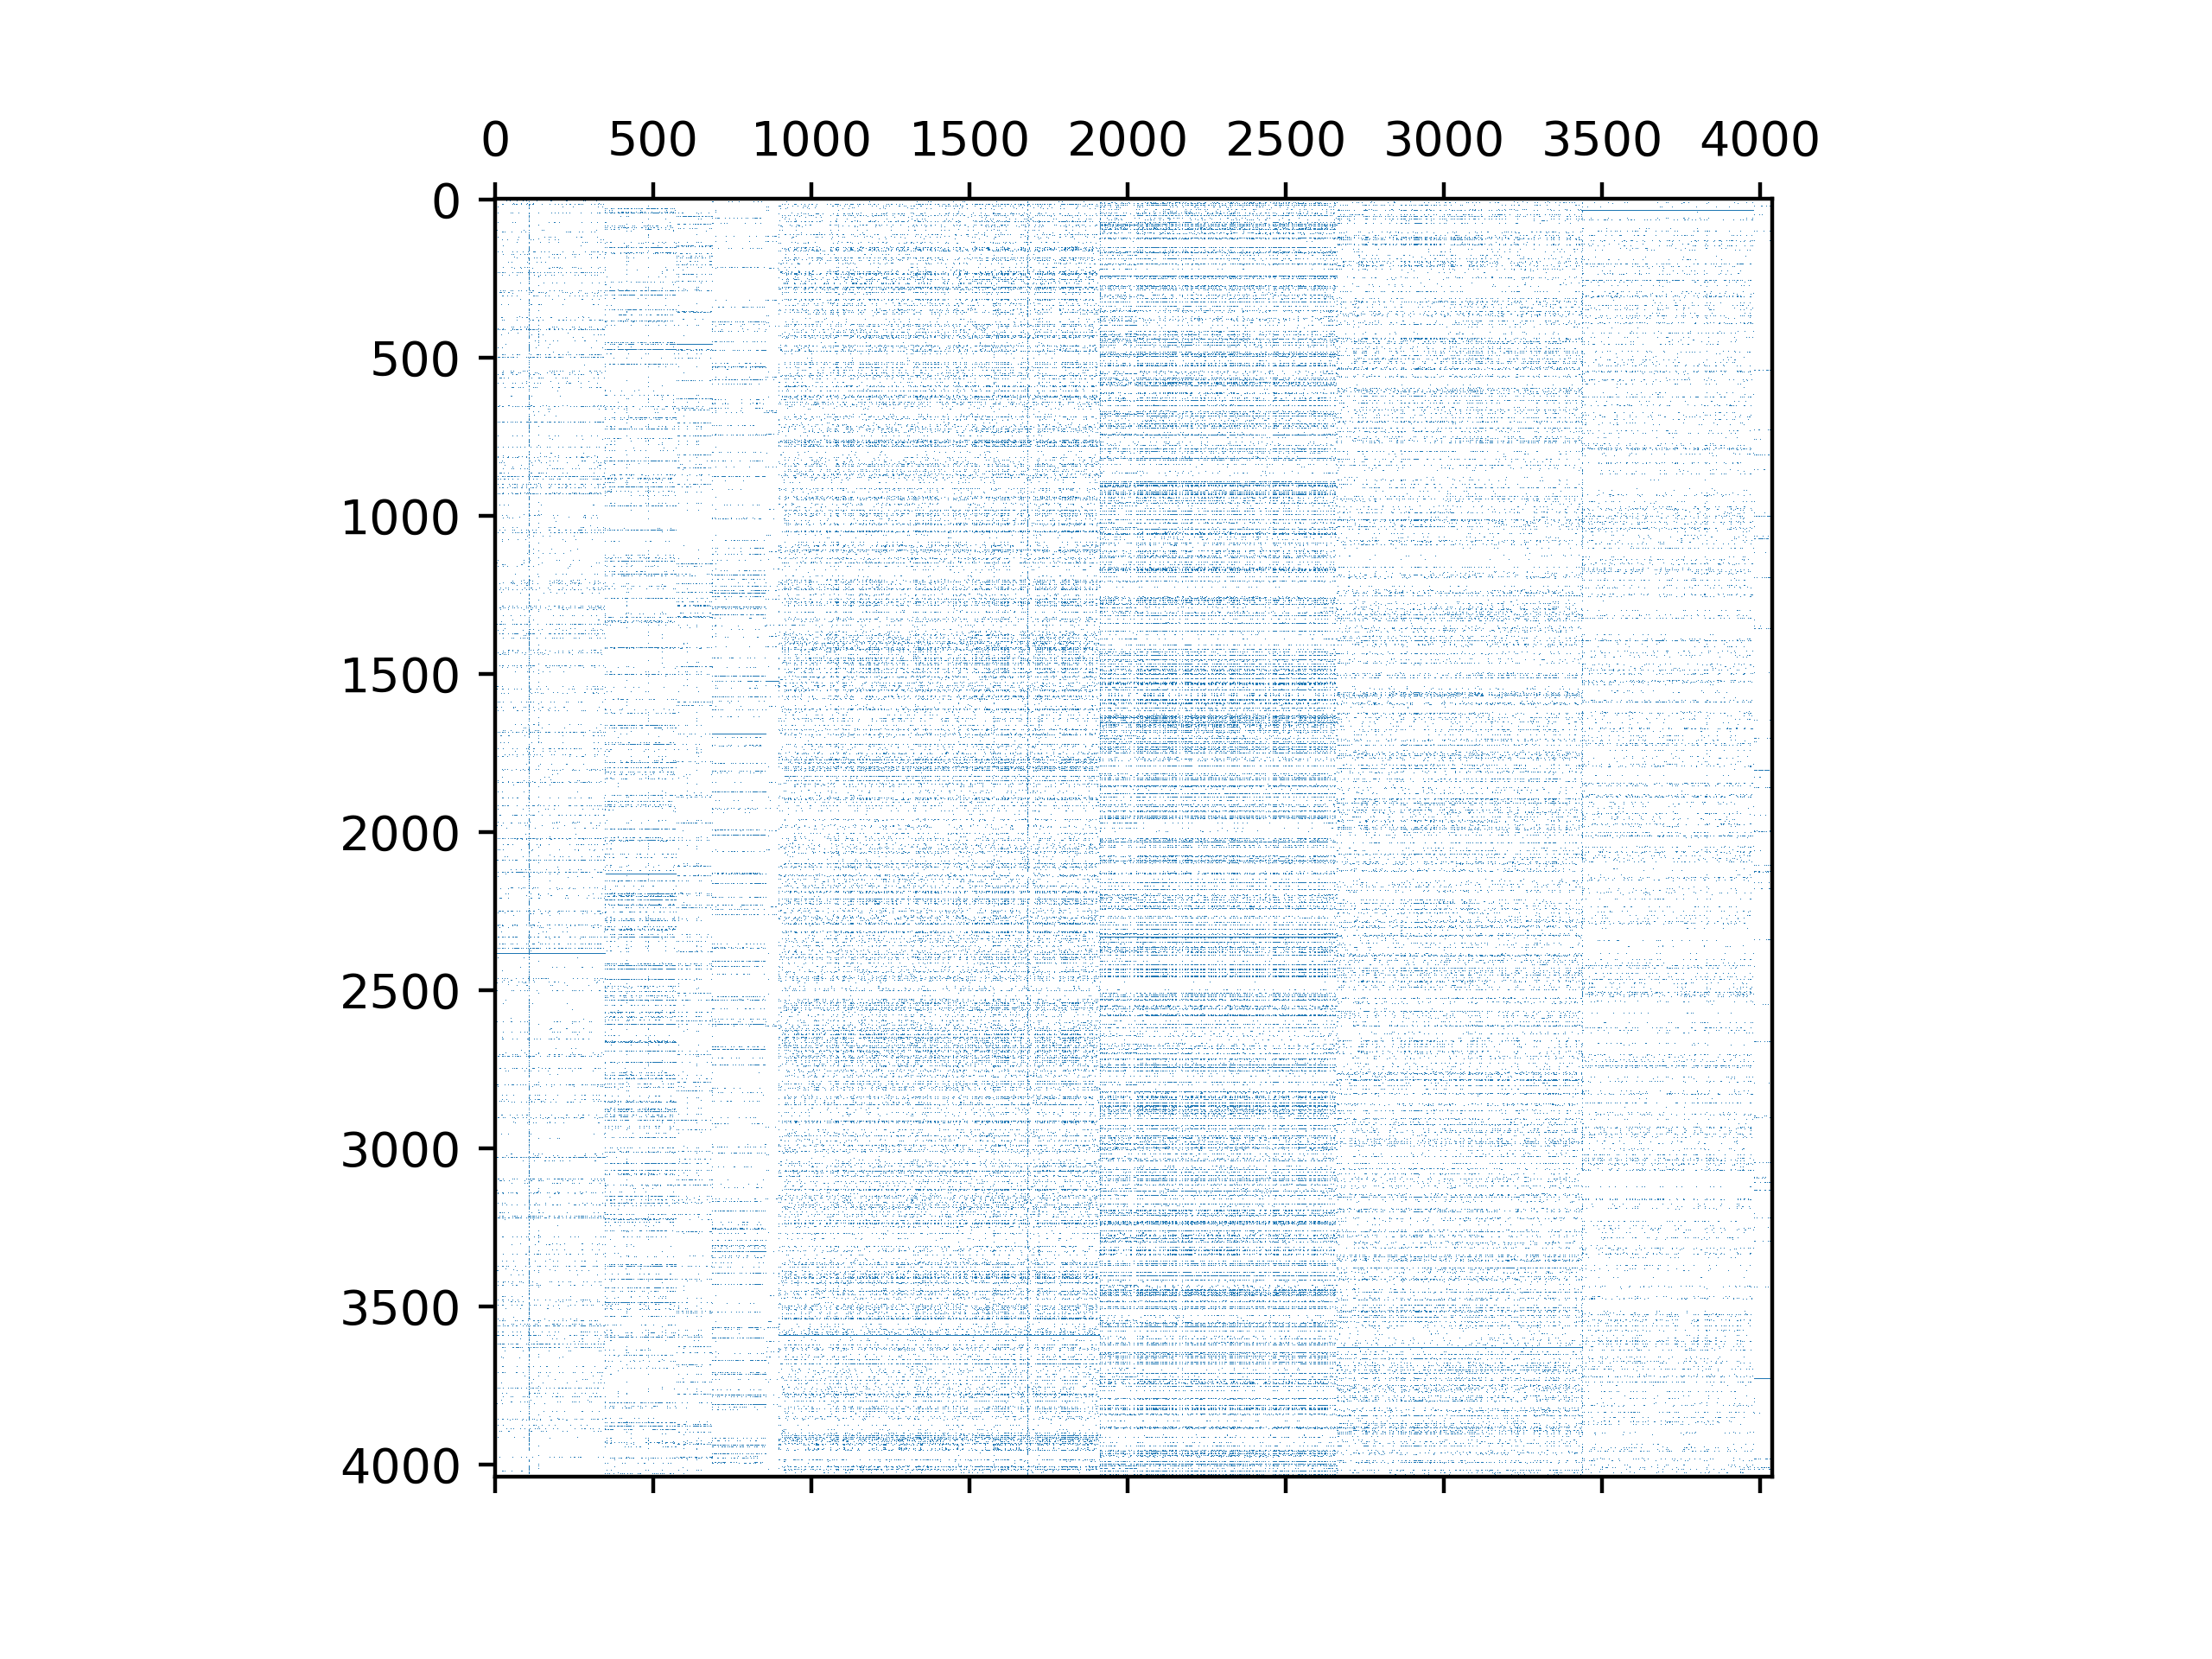
\includegraphics[width=5.5cm]{figures/fb-combined-rnd.png}}\hfil   
  \subfloat[Rabbit Order]{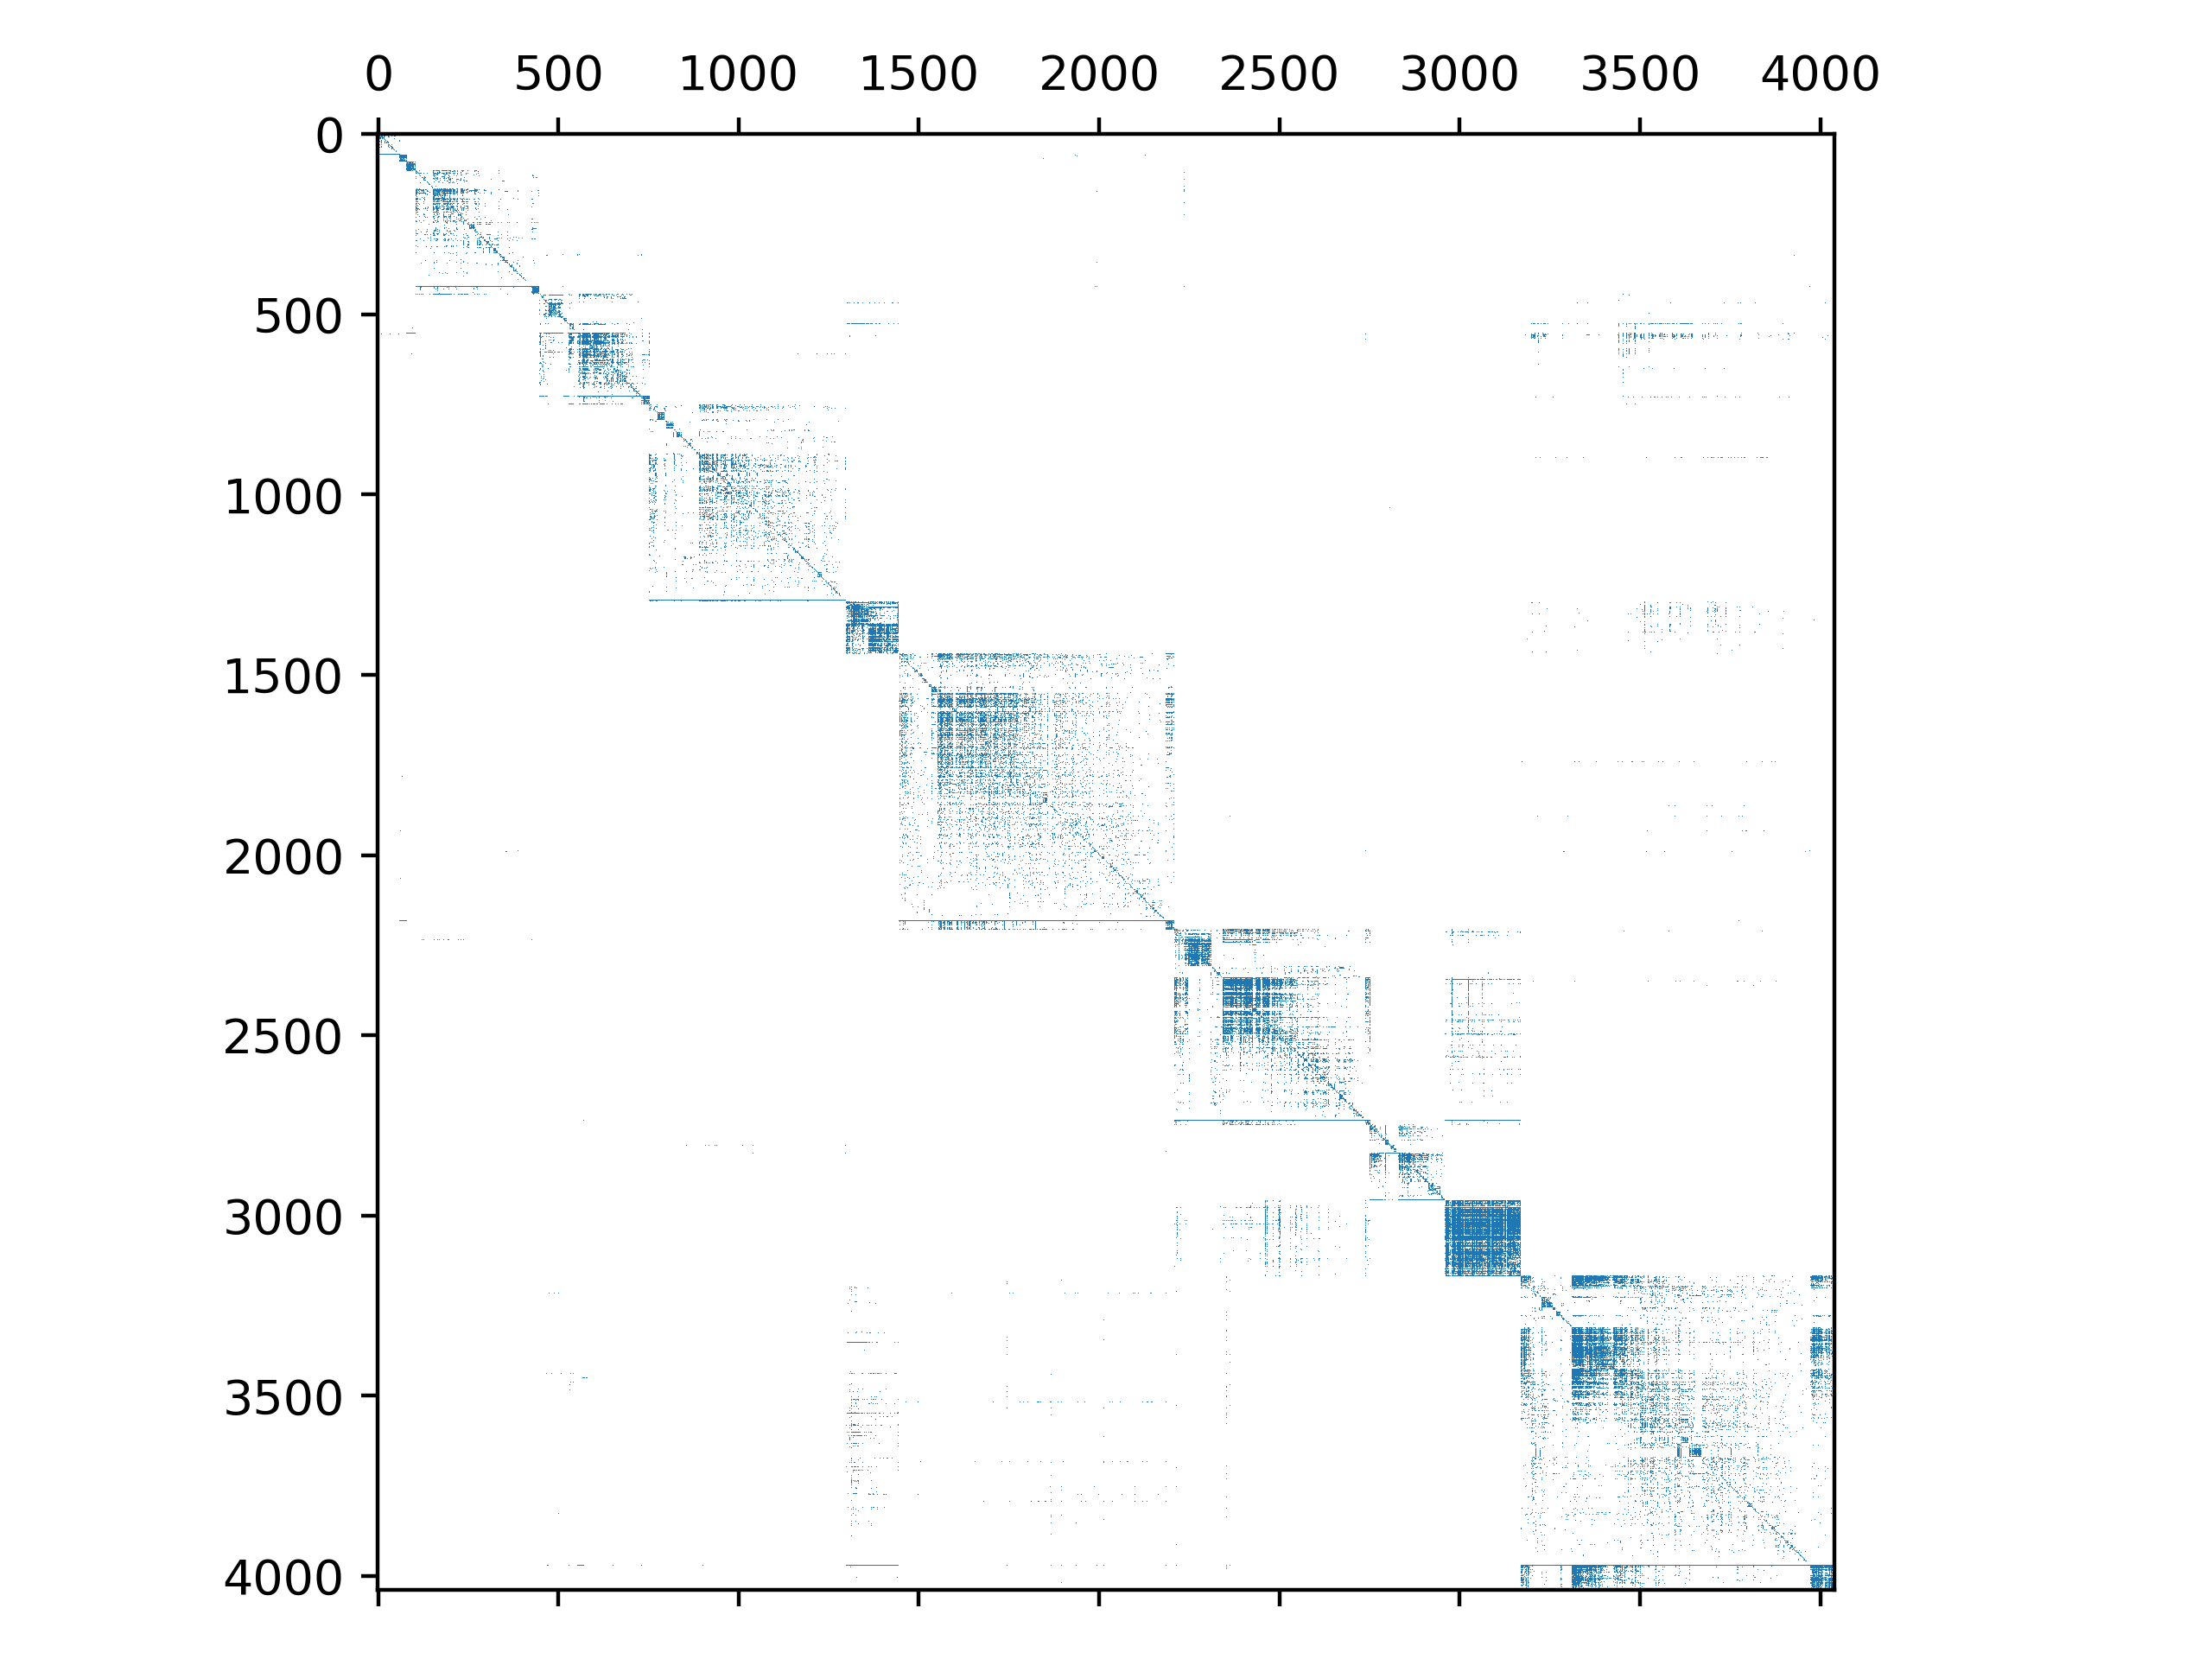
\includegraphics[width=5.5cm]{figures/fb-combined-rbt.png}}\hfil
  \subfloat[Cuthill-McKee Order]{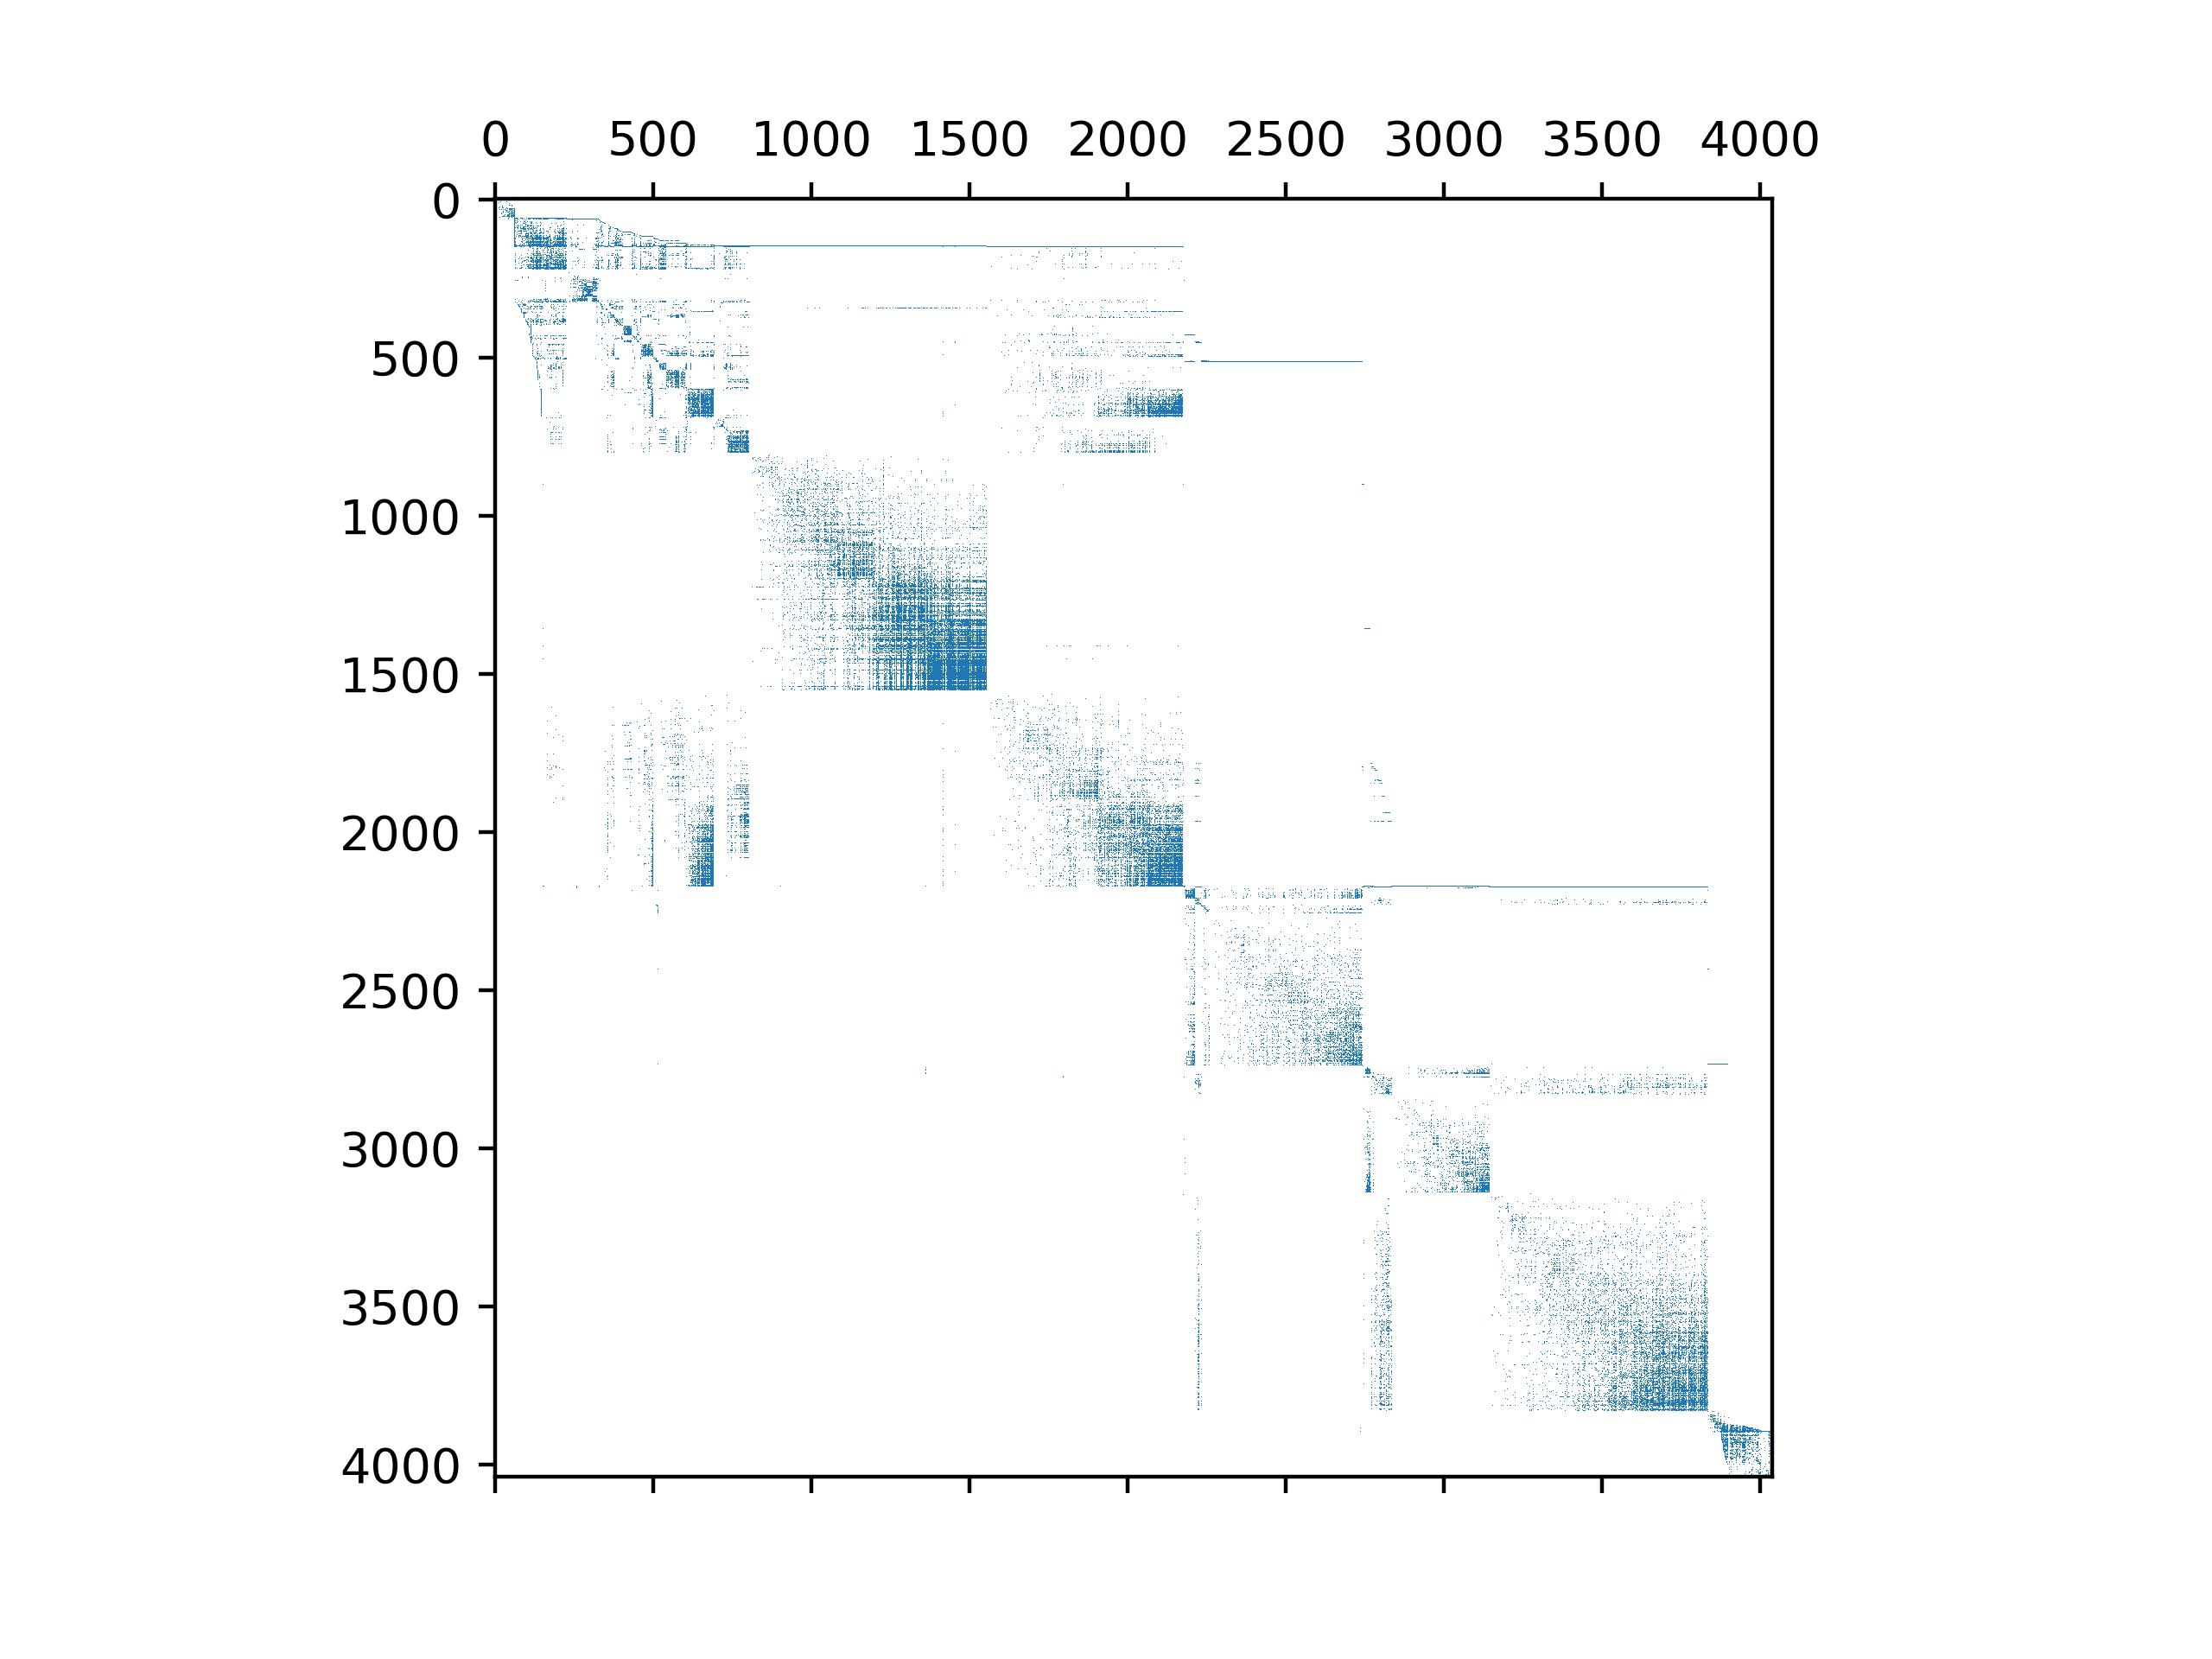
\includegraphics[width=5.5cm]{figures/fb-combined-rcm.png}}
  \caption{Adjacency matrices of an undirected Facebook Social Network graph with 4,039 vertices and 88,234 edges. Each pixel denotes an undirected edge (``friend-of'' relationship) between a pair of vertices (users) in the graph. Note the detected dense communities (submatrices) along the diagonal in (b) and the reduced bandwidth of the sparse matrix in (c). }\label{fig:fb_adjmats}
  \end{figure*}

This thesis is concerned in the interaction between Vertex and Edge ordering. Namely:

\textbf{RQ1}: It has been shown that using vertex and edge ordering to preprocess a graph confers performance benefits in a variety of applications. Is it possible to combine vertex
and edge ordering as a preprocessing step such that the performance benefit gained by the combination of both is compounded (i.e., is greater than using either separately)?
\begin{itemize}
  \item Can edge-centric graph traversal be sped up by first introducing some structure into the adjacency matrix?
\end{itemize}

\textbf{RQ2}: Given an arbitrary input graph, is there a \textit{vertex-and-edge} ordering combination that yields the best performance for an \ac{EC} traversal (measured in speed of execution and number of cache misses)?

This work answers these questions by making the following contributions. We:

\begin{enumerate}
  \item {Perform a preliminary performance evaluation on different vertex and edge orderings on single-threaded \ac{EC} traversals for a variety of graph datasets. We conclude that there \textit{does not} exist a one-size-fits-all \textit{vertex-and-edge} ordering that outperforms all others for all types of graphs.}
  \item {Derive an analytic model of performance using a dataset of graph features (statistical measures that summarize a graph), to identify the characteristics of a graph that help us determine which vertex-and-edge ordering performs best for \ac{EC} workloads.}
  \item {Develop a fully parallel implementation of the SlashBurn vertex ordering technique: \textbf{ParSB}.}
  \item {Propose a novel, lock-free, multithreaded vertex-and-edge ordering technique that leverages the compressed graph representation given by ParSB and traverses the edges of the graph using the \ac{HSFC}.}
  \item {Evaluate our novel vertex-and-edge ordering and compare its performance against locking-based and merging-based multithreaded \ac{EC} traversals.}
\end{enumerate}
%% The following is a directive for TeXShop to indicate the main file
%%!TEX root = diss.tex

\chapter{Abstract}

% This document provides brief instructions for using the \class{ubcdiss}
% class to write a \acs{UBC}-conformant dissertation in \LaTeX.  This
% document is itself written using the \class{ubcdiss} class and is
% intended to serve as an example of writing a dissertation in \LaTeX.
% This document has embedded \acp{URL} and is intended to be viewed
% using a computer-based \ac{PDF} reader.

% Note: Abstracts should generally try to avoid using acronyms.

% Note: at \ac{UBC}, both the \ac{GPS} Ph.D. defence programme and the
% Library's online submission system restricts abstracts to 350
% words.

% \ifgpscopy
%   This document was typeset in \texttt{gpscopy} mode.
% \else
%   This document was typeset in non-\texttt{gpscopy} mode.
% \fi

% Consider placing version information if you circulate multiple drafts
%\vfill
%\begin{center}
%\begin{sf}
%\fbox{Revision: \today}
%\end{sf}
%\end{center}
\par Graph structured data is used in a variety of applications because it naturally models ubiquitous concepts such as social networks, protein structures, and supply chains \cite{heidari2018scalable, yan2011applications}. This has motivated the development of \acp{GPS} whose aim is to process analytic queries such as PageRank, Shortest Paths, or Connected Components. Previous work accelerated graph processing by modifying the graph's data layout in memory \cite{rabbit, dbg, cost} or on disk \cite{mosaic, basc}. Since we typically describe a graph $G$ in terms of its Vertex and Edge sets using the notation $G(V, E)$, most \acp{GPS} can be categorized as \ac{VC} \cite{graphchi,flashgraph, basc} or \ac{EC} \cite{xstream} dependant on whether the systems implement analytical queries by applying a function over each vertex or each edge. 

\par In the \ac{VC} model, algorithms rely on user-defined vertex programs to compute analytic properties of an input graph. Vertex programs are run iteratively on every vertex in the graph. In each iteration, each vertex executes a user-defined vertex program, and messages are exchanged between neighbouring vertices to propagate updated vertex values. \ac{VC} systems reorder the \textit{vertices} of the graph to improve the locality of vertices that are expected to be frequently accessed together. 

\par In the \ac{EC} model, iteration occurs over the edges of the graph. For each edge in the graph, we apply an update to either the source or destination vertex incident on that edge. \ac{EC} systems reorder the \textit{edges} of the graph to mitigate the random-access pattern of incident vertices that is common to many graph processing kernels such as PageRank.

\par One way of representing a graph is as a square $N \times N$ matrix, $A$, where $N= |V|$. A non-zero element $A_{i, j}$ indicates the existence of an edge from vertex $i$ to vertex $j$. Real-world graphs are typically sparse \cite{listingkcliques}, meaning that the number of edges, $M=|E|$, is much smaller than the number of possible edges in the graph: $M\ll M_{\max} = {N \choose 2}$. 

\par \ac{EC} systems that order the edges of the graph by ascending \textit{Source} or \textit{Destination} ID effectively iterate over $A$ in Row-major or Column-major order, respectively. If we traverse the adjacency matrix of a graph in Row-major order, we will have excellent locality in the source vertices (since we will process all outgoing neighbours of a source vertex before moving on to the next source vertex), but our access to the destination vertex of each outgoing edge will correspond to near-random memory accesses of the vertex array. Prior work \cite{cost} addressed this concern by using an edge ordering defined by the \ac{HSFC}, which is a way of assigning indices to the edges of a graph that produces locality in \textit{both} the source and destination vertices. 

\par \ac{VC} systems can use vertex reordering as a preprocessing optimization to improve the memory access locality of the vertices. For example, certain \ac{VC} systems \cite{dbg, cagra} use the degrees of the vertices to cluster and/or sort the vertices (e.g., sorting the vertices by descending order of degree). The rationale for this is that high degree vertices (also known as ``Hub'' vertices) are, by definition, neighbours of a large number of vertices. These hubs will be frequently accessed when iterating over the edge set of the graph \cite{lwr}. A descending degree sort collocates these hub vertices in memory and increases the likelihood of frequently accessed vertices being cached. Alternatively, Rabbit Order \cite{rabbit} relies on the observation that many real-world graphs such as social networks contain community structures, where vertices that belong to the same community share a larger number of edges than vertices that belong to different communities. The goal of Rabbit Order is to order the vertices in such a way that consecutive vertex IDs correspond to meaningful communities. The algorithm first detects these communities and then labels the vertices according to those communities. 

\par A vertex reordering can be thought of as a function that maps each vertex ID to a new ID in the range: $[0, N)$. This mapping or relabeling is known as a \textit{graph isomorphism}, since all edges between vertices are preserved and the structure of the graph is unchanged. However, vertex reordering can impose ``structure'' on the adjacency matrix of the graph. Figure \ref{fig:fb_adjmats} shows the adjacency matrix of a Facebook social network graph that was constructed from the data of survey participants using the Facebook App \cite{leskovec2012learning}. The graph has been reordered using 3 vertex orders: a random vertex ID assignment, and the IDs calculated using Rabbit and Cuthill-McKee orders. 

\begin{figure*}[!htp]

  \centering
  \subfloat[Random Order]{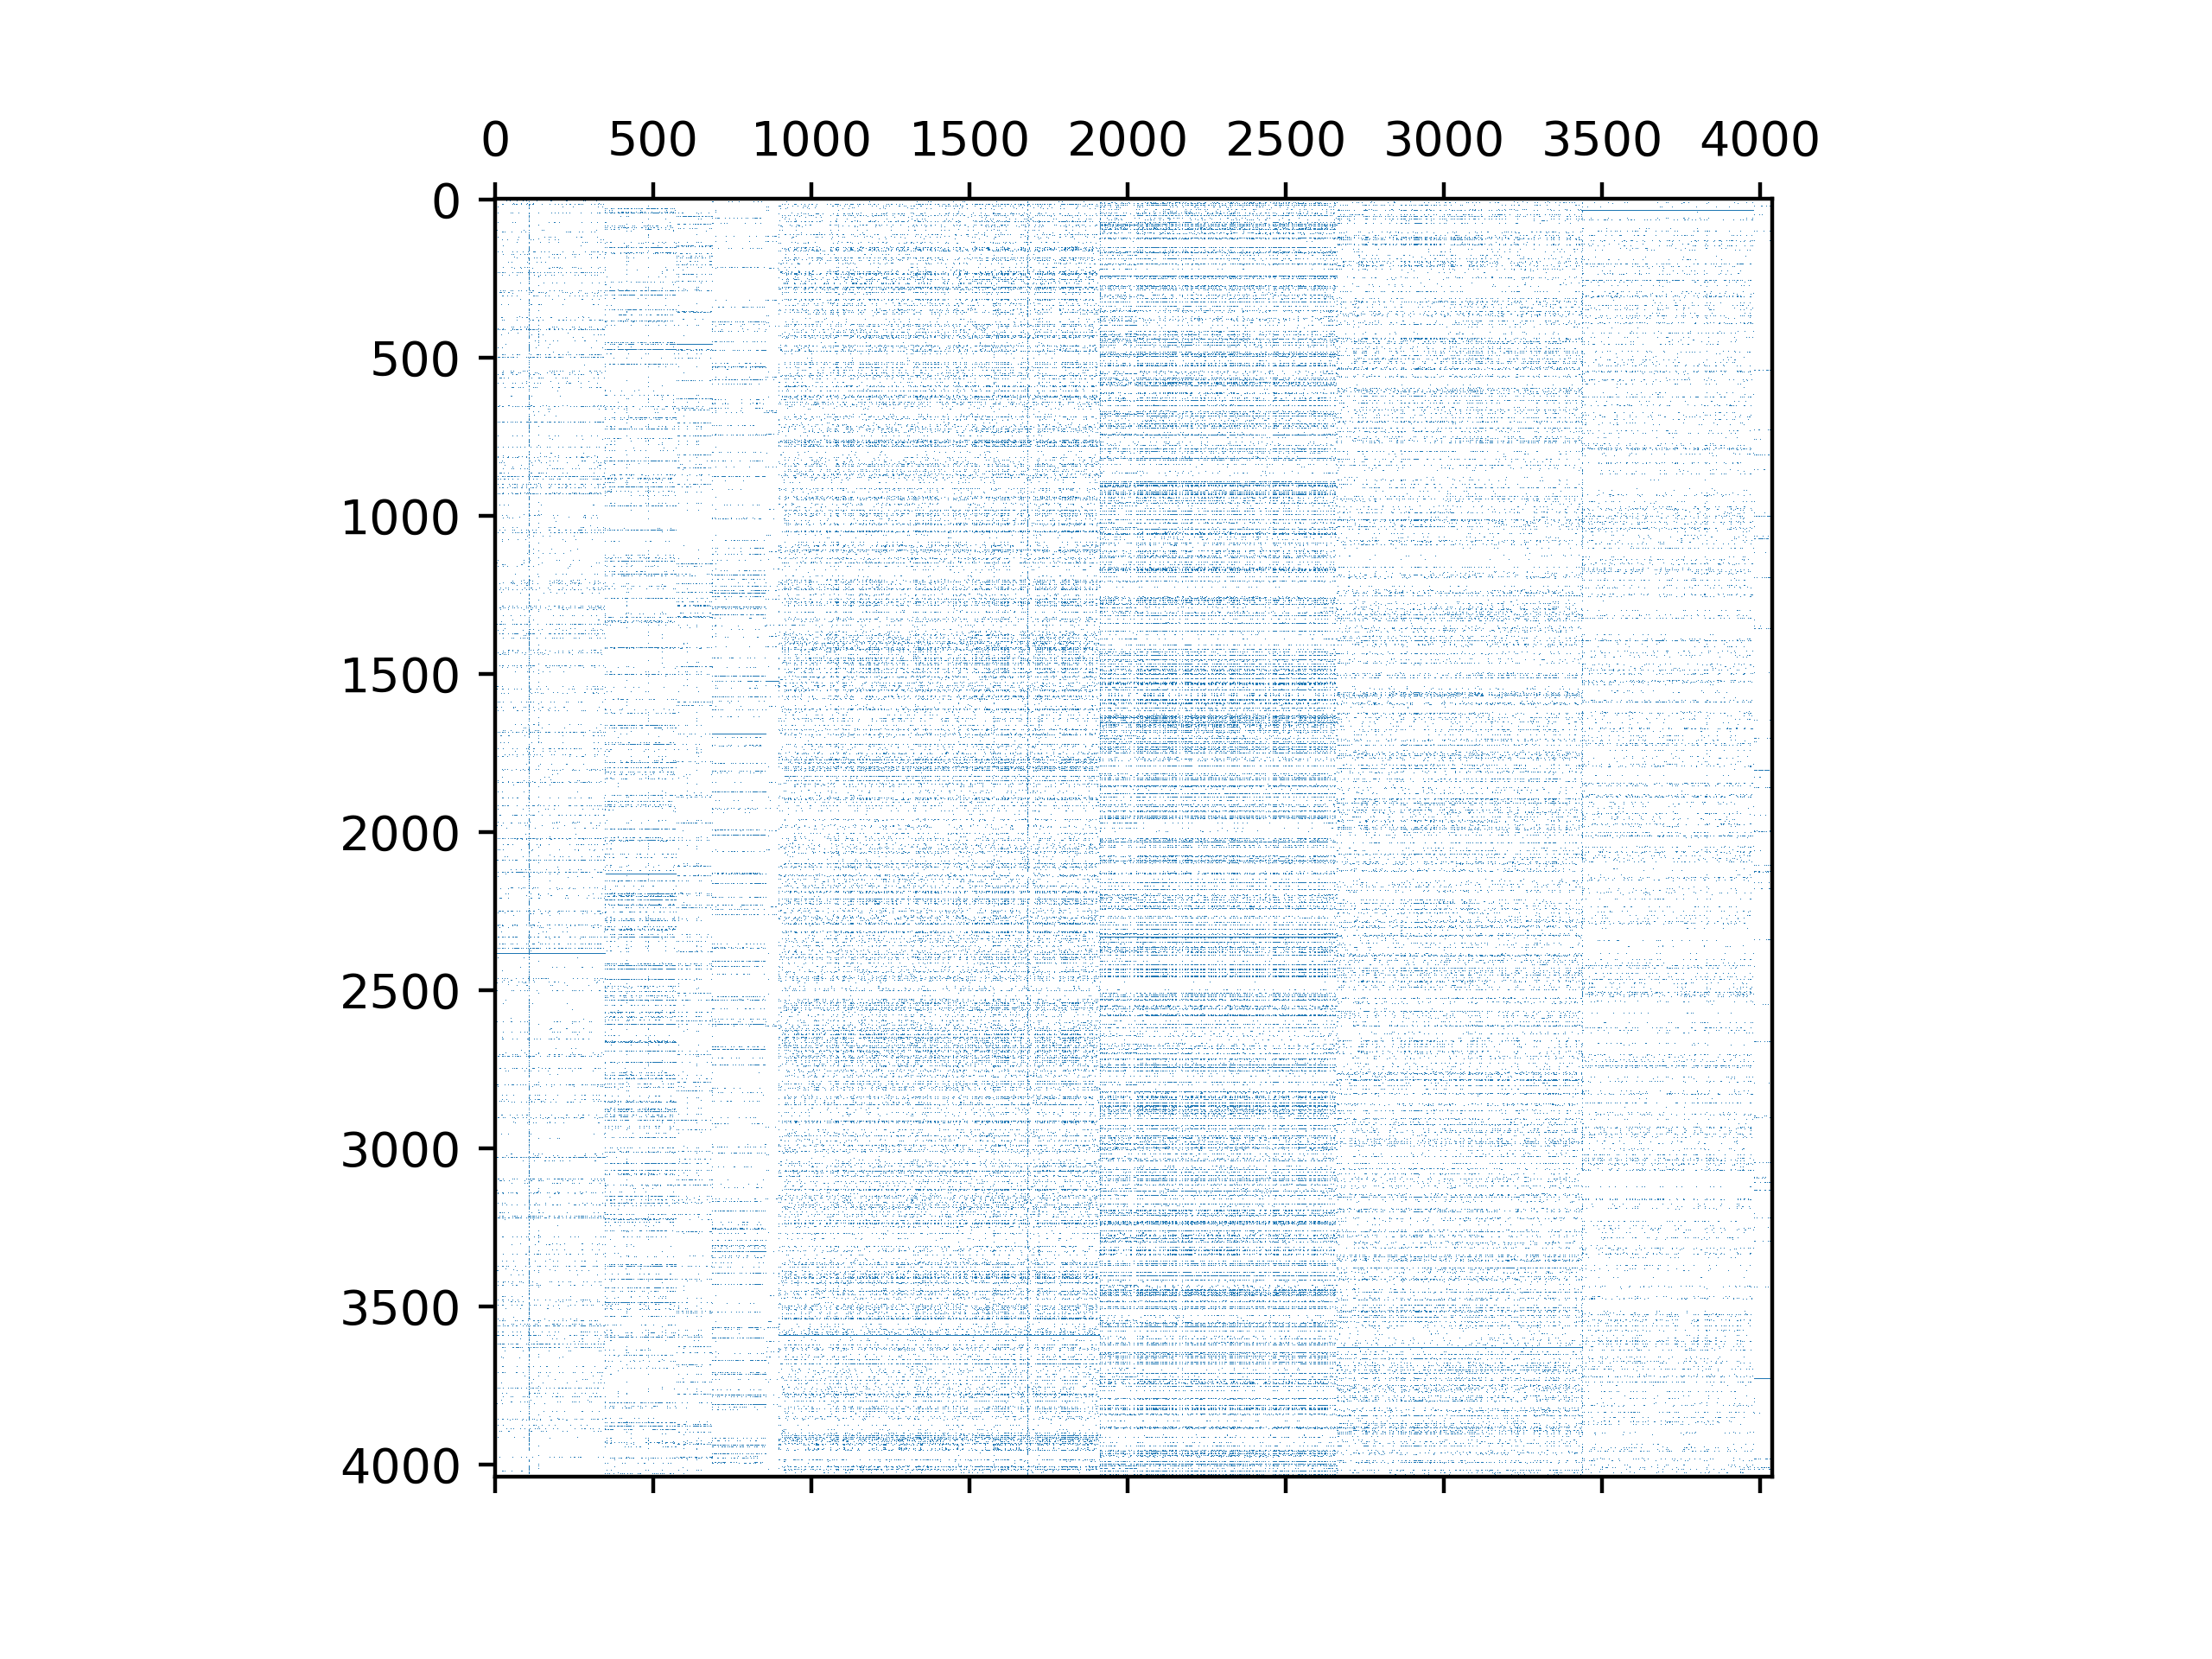
\includegraphics[width=5.5cm]{figures/fb-combined-rnd.png}}\hfil   
  \subfloat[Rabbit Order]{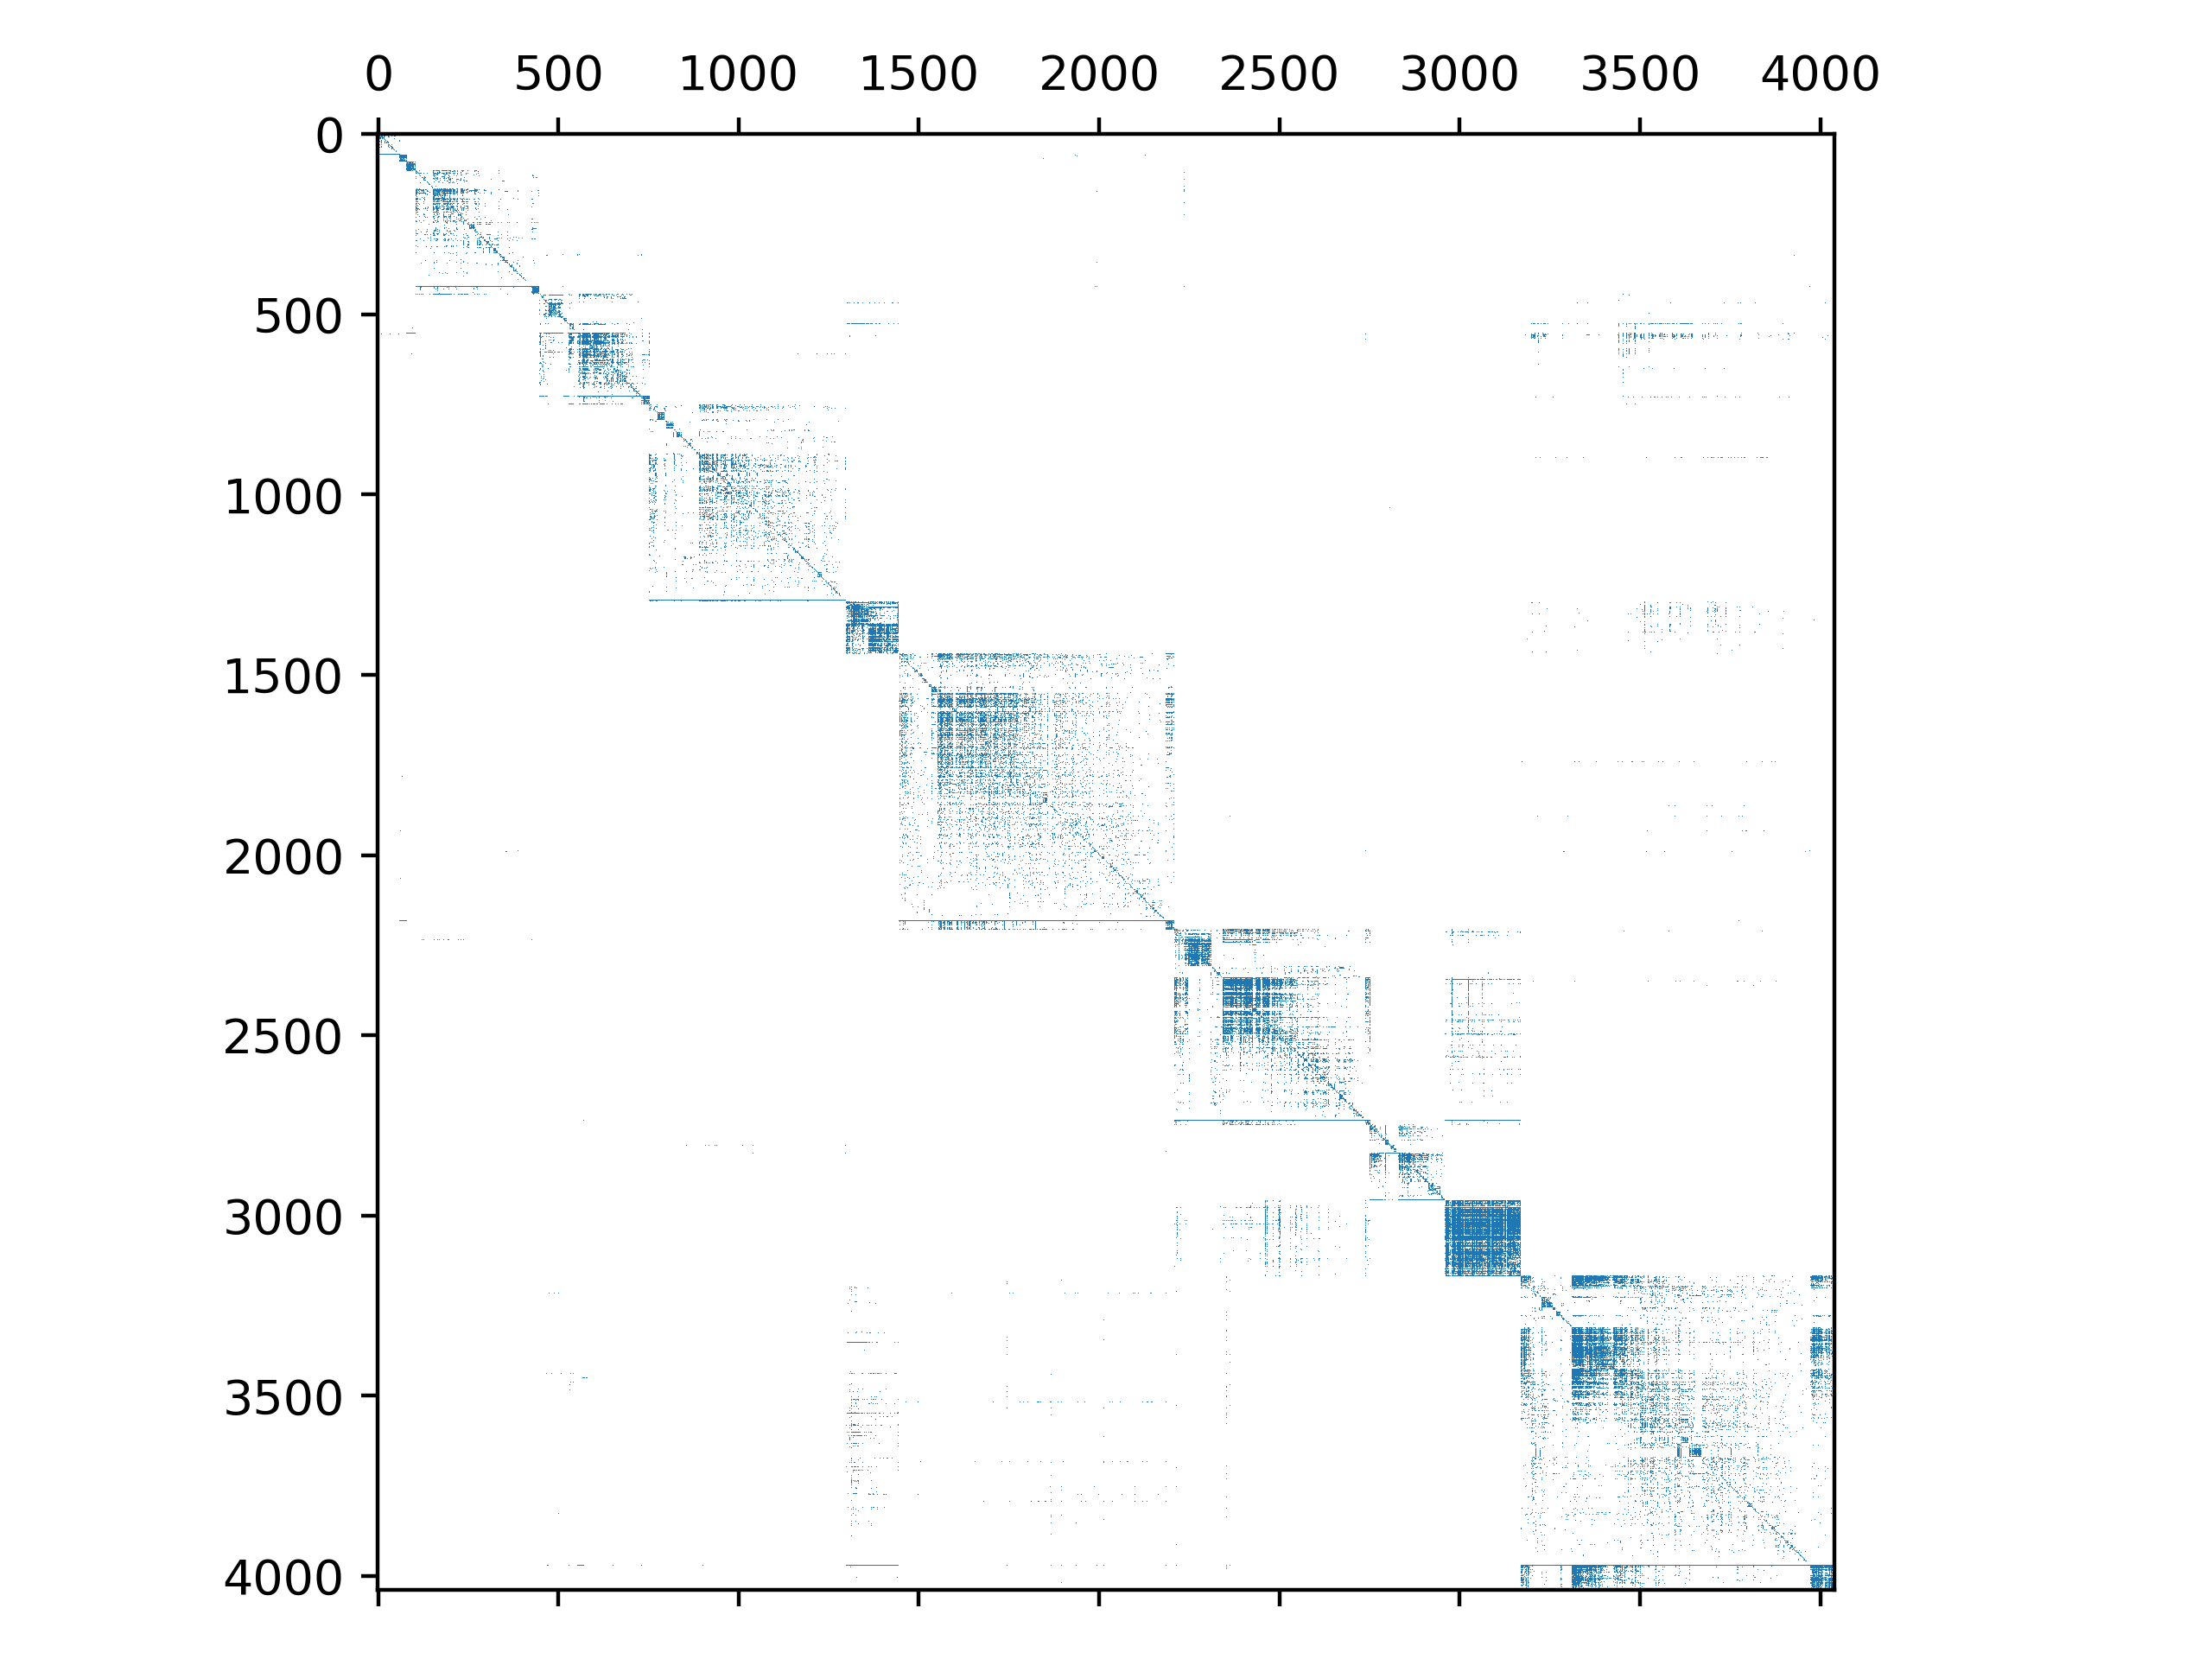
\includegraphics[width=5.5cm]{figures/fb-combined-rbt.png}}\hfil
  \subfloat[Cuthill-McKee Order]{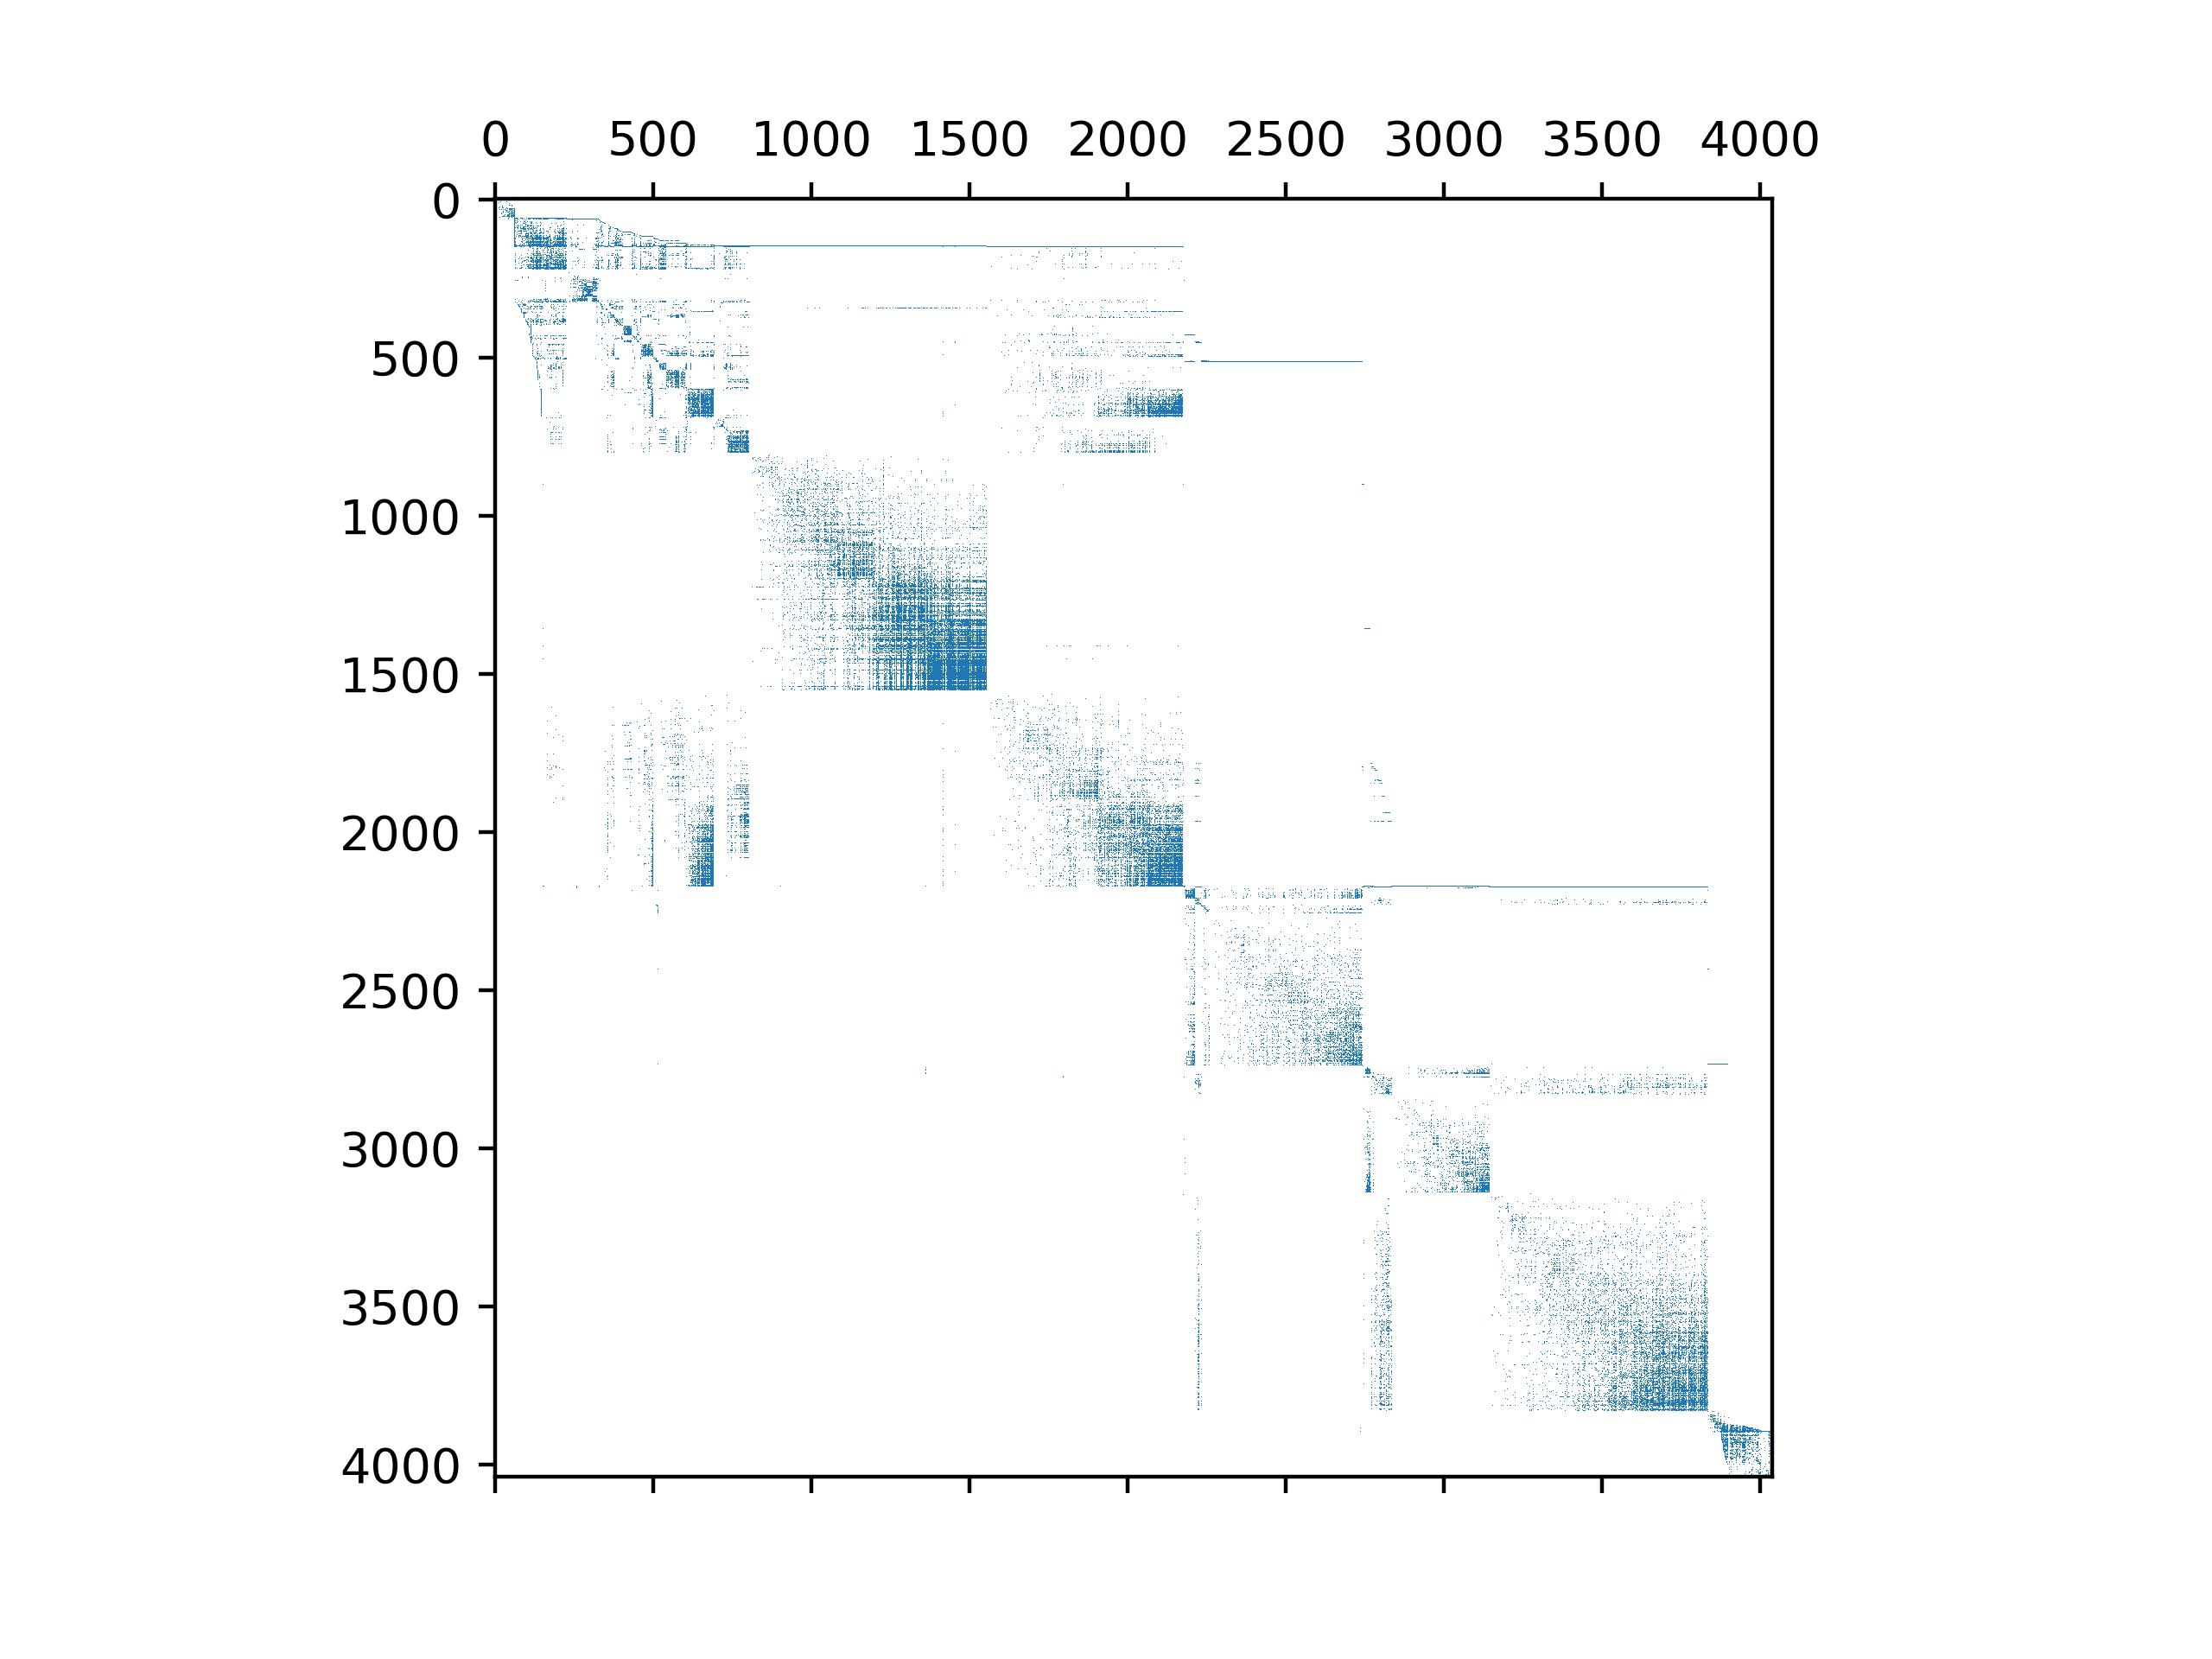
\includegraphics[width=5.5cm]{figures/fb-combined-rcm.png}}
  \caption{Adjacency matrices of an undirected Facebook Social Network graph with 4,039 vertices and 88,234 edges. Each pixel denotes an undirected edge (``friend-of'' relationship) between a pair of vertices (users) in the graph. Note the detected dense communities (submatrices) along the diagonal in (b) and the reduced bandwidth of the sparse matrix in (c). }\label{fig:fb_adjmats}
  \end{figure*}

To date, researchers have looked at \textit{either} vertex or edge ordering to optimize the performance of their \ac{VC} or \ac{EC} systems, but there has not been an extensive evaluation of possible \textit{vertex-and-edge} orderings. We define a \textbf{Vertex-and-Edge Ordering} of a graph as a preprocessing algorithm that:
\begin{enumerate}
    \item Reorders the \textit{vertices} of the graph in order to introduce structure into the adjacency matrix.\item The \textit{edges} are traversed using an edge ordering that leverages the structure of the isomorphic adjacency matrix. The edge ordering ignores large empty regions of the adjacency matrix and traverses the dense regions that were introduced using the vertex ordering using the \ac{HSFC}.
\end{enumerate}
This thesis is concerned in filling this knowledge gap and investigates the interaction between Vertex and Edge ordering. Namely, we answer the following research questions:

\textbf{RQ1}: It has been shown that vertex and edge ordering confer performance benefits in a variety of applications. Is it possible to combine vertex
and edge ordering as a preprocessing step such that the performance benefit gained by the combination of both is compounded (i.e., is greater than using either separately)?
\begin{itemize}
  \item Can edge-centric graph traversal be sped up by first introducing some structure into the adjacency matrix?
\end{itemize}

\textbf{RQ2}: Given an arbitrary input graph, is there a \textit{vertex-and-edge} ordering combination that yields the best performance for an \ac{EC} traversal (measured in speed of execution and number of cache misses)?

We answer these questions by making the following contributions. We:

\begin{enumerate}
  \item {Perform a preliminary performance evaluation on different vertex and edge orderings on single-threaded \ac{EC} traversals for a variety of graph datasets. We conclude that there \textit{does not} exist a one-size-fits-all \textit{vertex-and-edge} ordering that outperforms all others for all types of graphs.}
  \item {Derive an analytic model of performance using a dataset of graph features (statistical measures that summarize a graph) to identify the characteristics of a graph that help us determine which vertex-and-edge ordering performs best for \ac{EC} workloads.}
  \item {Develop a fully parallel implementation of the SlashBurn vertex ordering technique: \textbf{ParSB}.}
  \item {Propose a novel, lock-free, multithreaded vertex-and-edge ordering technique that leverages the compressed graph representation given by ParSB and traverses the edges of the graph using the \ac{HSFC}.}
  \item {Evaluate our novel vertex-and-edge ordering and compare its performance against locking-based and merging-based multithreaded vertex-and-edge orderings.}
\end{enumerate}
\cleardoublepage

%    4. Lay Summary (Effective May 2017, mandatory - maximum 150 words)
\include{laysummary}
\cleardoublepage

%    5. Preface
\include{preface}
\cleardoublepage

%    6. Table of contents (mandatory - list all items in the preliminary pages
%    starting with the abstract, followed by chapter headings and
%    subheadings, bibliographies and appendices)
\tableofcontents
\cleardoublepage	% required by tocloft package

%    7. List of tables (mandatory if thesis has tables)
\listoftables
\cleardoublepage	% required by tocloft package

%    8. List of figures (mandatory if thesis has figures)
\listoffigures
\cleardoublepage	% required by tocloft package

%    9. List of illustrations (mandatory if thesis has illustrations)
%   10. Lists of symbols, abbreviations or other (optional)

%   11. Glossary (optional)
%% The following is a directive for TeXShop to indicate the main file
%%!TEX root = diss.tex

\chapter{Glossary}

This glossary uses the handy \latexpackage{acroynym} package to automatically
maintain the glossary.  It uses the package's \texttt{printonlyused}
option to include only those acronyms explicitly referenced in the
\LaTeX\ source.  To change how the acronyms are rendered, change the
\verb+\acsfont+ definition in \verb+diss.tex+.

% use \acrodef to define an acronym, but no listing
\acrodef{UI}{user interface}
\acrodef{UBC}{University of British Columbia}

% The acronym environment will typeset only those acronyms that were
% *actually used* in the course of the document
\begin{acronym}[ANOVA]
\acro{ANOVA}[ANOVA]{Analysis of Variance\acroextra{, a set of
  statistical techniques to identify sources of variability between groups}}
\acro{API}{application programming interface}
\acro{CTAN}{\acroextra{The }Common \TeX\ Archive Network}
\acro{DOI}{Document Object Identifier\acroextra{ (see
    \url{http://doi.org})}}
\acro{GPS}[GPS]{Graduate and Postdoctoral Studies}
\acro{PDF}{Portable Document Format}
\acro{RCS}[RCS]{Revision control system\acroextra{, a software
    tool for tracking changes to a set of files}}
\acro{TLX}[TLX]{Task Load Index\acroextra{, an instrument for gauging
  the subjective mental workload experienced by a human in performing
  a task}}
\acro{UML}{Unified Modelling Language\acroextra{, a visual language
    for modelling the structure of software artefacts}}
\acro{URL}{Unique Resource Locator\acroextra{, used to describe a
    means for obtaining some resource on the world wide web}}
\acro{W3C}[W3C]{\acroextra{the }World Wide Web Consortium\acroextra{,
    the standards body for web technologies}}
\acro{XML}{Extensible Markup Language}
\acro{GPS}{Graph Processing System}
\acrodefplural{GPS}[GPS]{Graph Processing Systems}
\acro{VC}{Vertex-Centric}
\acro{EC}{Edge-Centric}
\acro{HSFC}{Hilbert Space Filling Curve}
\acro{CM}{Cuthill-McKee}
\acro{RCM}{Reverse Cuthill-McKee}
\end{acronym}

% You can also use \newacro{}{} to only define acronyms
% but without explictly creating a glossary
% 
% \newacro{ANOVA}[ANOVA]{Analysis of Variance\acroextra{, a set of
%   statistical techniques to identify sources of variability between groups.}}
% \newacro{API}[API]{application programming interface}
% \newacro{GOMS}[GOMS]{Goals, Operators, Methods, and Selection\acroextra{,
%   a framework for usability analysis.}}
% \newacro{TLX}[TLX]{Task Load Index\acroextra{, an instrument for gauging
%   the subjective mental workload experienced by a human in performing
%   a task.}}
% \newacro{UI}[UI]{user interface}
% \newacro{UML}[UML]{Unified Modelling Language}
% \newacro{W3C}[W3C]{World Wide Web Consortium}
% \newacro{XML}[XML]{Extensible Markup Language}
	% always input, since other macros may rely on it

\textspacing		% begin one-half or double spacing

%   12. Acknowledgements (optional)
\include{ack}

%   13. Dedication (optional)

% Body of Thesis (not all sections may apply)
\mainmatter

\acresetall	% reset all acronyms used so far


%    1. Introduction
%% The following is a directive for TeXShop to indicate the main file
%%!TEX root = diss.tex

\chapter{Introduction}
\label{ch:Introduction}

% \begin{epigraph}
%     \emph{If I have seen farther it is by standing on the shoulders of
%     Giants.} ---~Sir Isaac Newton (1855)
% \end{epigraph}


\par Graph structured data is used in a variety of applications because it naturally models ubiquitous concepts such as social networks, protein structures, and supply chains \cite{heidari2018scalable, yan2011applications}. This has motivated the development of \acp{GPS} whose aim is to process analytic queries such as PageRank, Shortest Paths, or Connected Components. Previous work accelerated graph processing by modifying the graph's data layout in memory \cite{rabbit, dbg, cost} or on disk \cite{mosaic, basc}. We typically describe a graph $G$ in terms of its Vertex and Edge sets using the notation $G(V, E)$. Correspondingly, most \acp{GPS} can be categorized as \ac{VC} \cite{graphchi,flashgraph, basc} or \ac{EC} \cite{xstream}, depending on whether the systems implement analytical queries by applying a function over each vertex or each edge. 

\par In the \ac{VC} model, algorithms rely on user-defined vertex programs to compute analytic properties of an input graph. Vertex programs are run iteratively on every vertex in the graph. In each iteration, each vertex executes a user-defined vertex program, and messages are exchanged between neighbouring vertices to propagate updated vertex values. \ac{VC} systems reorder the \textit{vertices} of the graph to improve the locality of vertices that are expected to be frequently accessed together. 

\par In the \ac{EC} model, iteration occurs over the edges of the graph. For each edge in the graph, we apply an update to either the source or destination vertex incident on that edge. \ac{EC} systems reorder the \textit{edges} of the graph to mitigate the random-access pattern of incident vertices that is common to many graph processing kernels such as PageRank.

\par One way of representing a graph is with a square $N \times N$ adjacency matrix, $A$, where $N= |V|$. A non-zero element $A_{i, j}$ indicates the existence of an edge from vertex $i$ to vertex $j$. Real-world graphs are typically sparse \cite{listingkcliques}, meaning that the number of edges, $M=|E|$, is much smaller than the number of possible edges in the graph: $M\ll M_{\max} = {N \choose 2}$. Equivalently, this means that the adjacency matrix of a typical real-world graph will be mostly filled with zeroes. 

\par \ac{EC} systems that order the edges of the graph by ascending \textit{Source} or \textit{Destination} ID effectively iterate over $A$ in Row-major or Column-major order, respectively. If we traverse the adjacency matrix of a graph in Row-major order, we will have excellent locality in the source vertices (since we will process all outgoing neighbours of a source vertex before moving on to the next source vertex), but our access to the destination vertex of each outgoing edge will correspond to near-random memory accesses of the vertex array. Prior work \cite{cost} addressed this concern by using an edge ordering defined by the \ac{HSFC}, which is a way of assigning indices to the edges of a graph that produces locality in \textit{both} the source and destination vertices. 

\par \ac{VC} systems can use vertex reordering as a preprocessing optimization to improve the memory access locality of the vertices. For example, certain \ac{VC} systems \cite{dbg, cagra} use the degrees of the vertices to cluster and/or sort the vertices (e.g., sorting the vertices by descending order of degree). The rationale for this is that high degree vertices (also known as ``Hub'' vertices) are, by definition, neighbours of a large number of vertices. These hubs will be frequently accessed when iterating over the edge set of the graph \cite{lwr}. A descending degree sort collocates these hub vertices in memory and increases the likelihood of frequently accessed vertices being cached. Alternatively, Rabbit Order \cite{rabbit} relies on the observation that many real-world graphs such as social networks contain community structures, where vertices that belong to the same community share a larger number of edges than vertices that belong to different communities. The goal of Rabbit Order is to order the vertices in such a way that consecutive vertex IDs correspond to meaningful communities. The algorithm first detects these communities and then labels the vertices according to those communities. 

\par A vertex reordering can be thought of as a function that maps each vertex ID to a new ID in the range: $[0, N)$. This mapping or relabeling is known as a \textit{graph isomorphism}, since all edges between vertices are preserved and the structure of the graph is unchanged. However, vertex reordering can impose ``structure'' on the adjacency matrix of the graph. Figure \ref{fig:fb_adjmats} shows the adjacency matrix of a Facebook social network graph that was constructed from the data of survey participants using the Facebook App \cite{leskovec2012learning}. The graph has been reordered using 3 vertex orders: a random vertex ID assignment, and the IDs calculated using the Rabbit and Cuthill-McKee orders. 

\begin{figure*}[!htp]

  \centering
  \subfloat[Random Order]{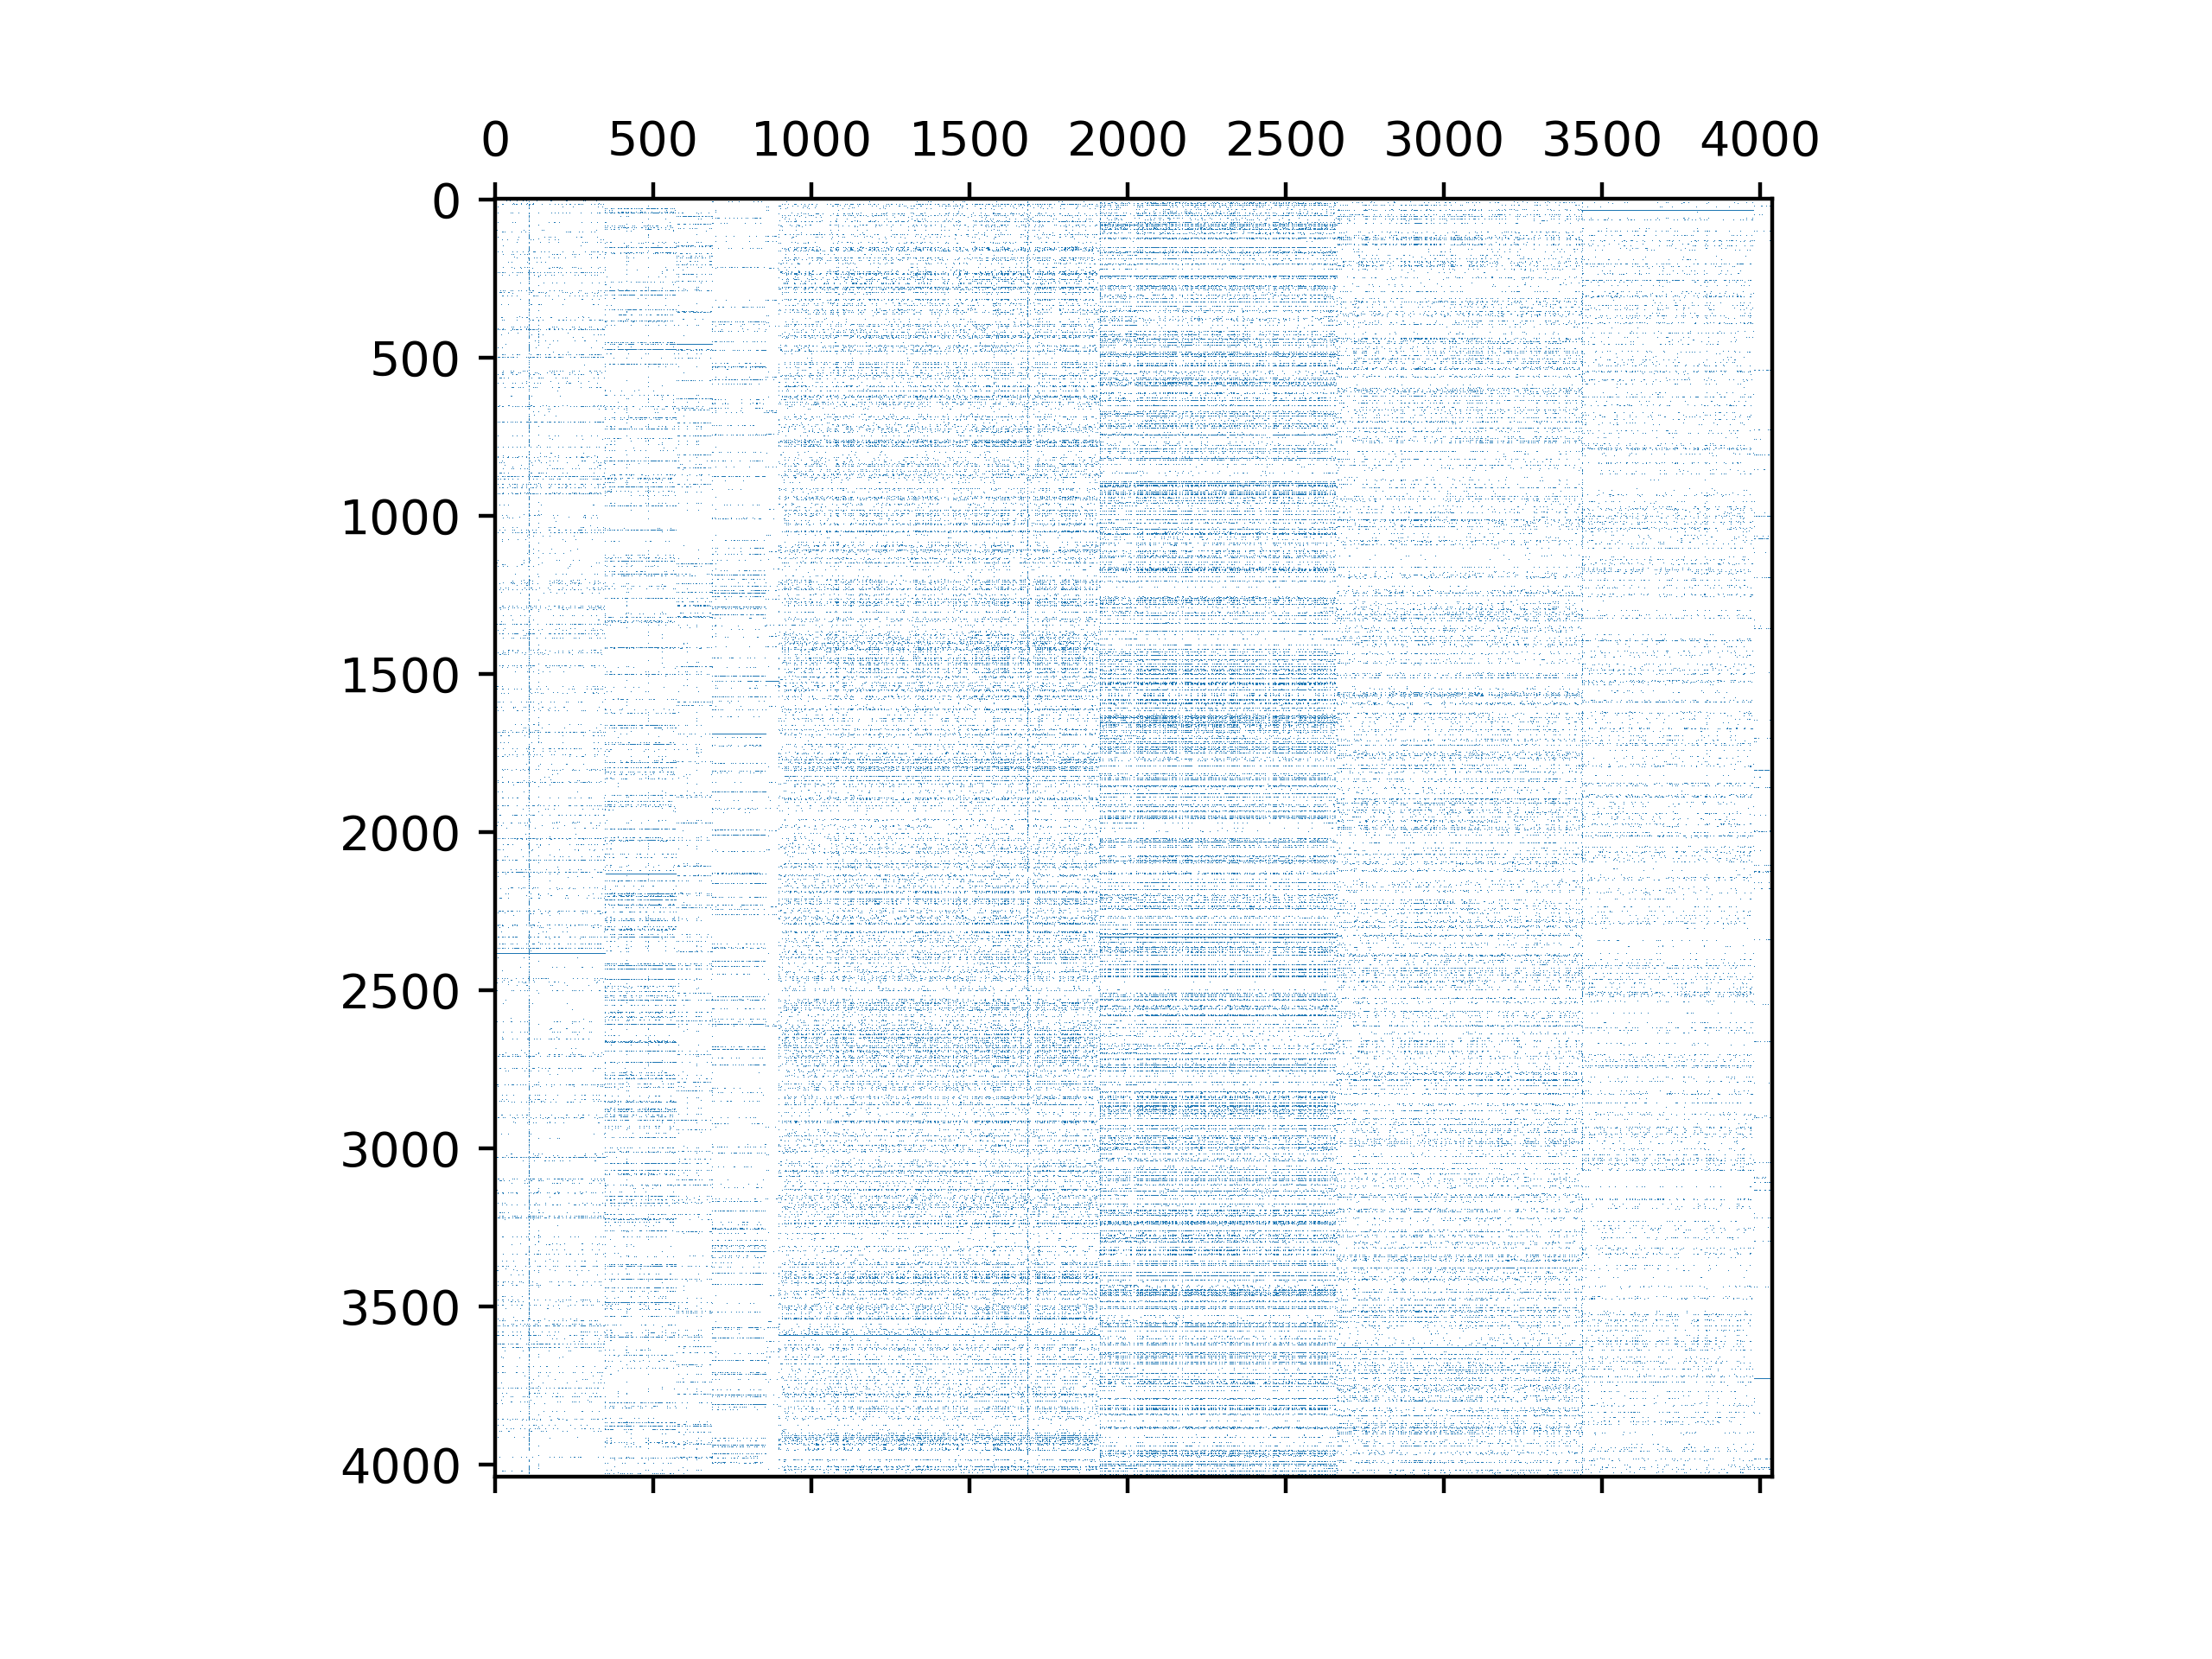
\includegraphics[width=5.5cm]{figures/fb-combined-rnd.png}}\hfil   
  \subfloat[Rabbit Order]{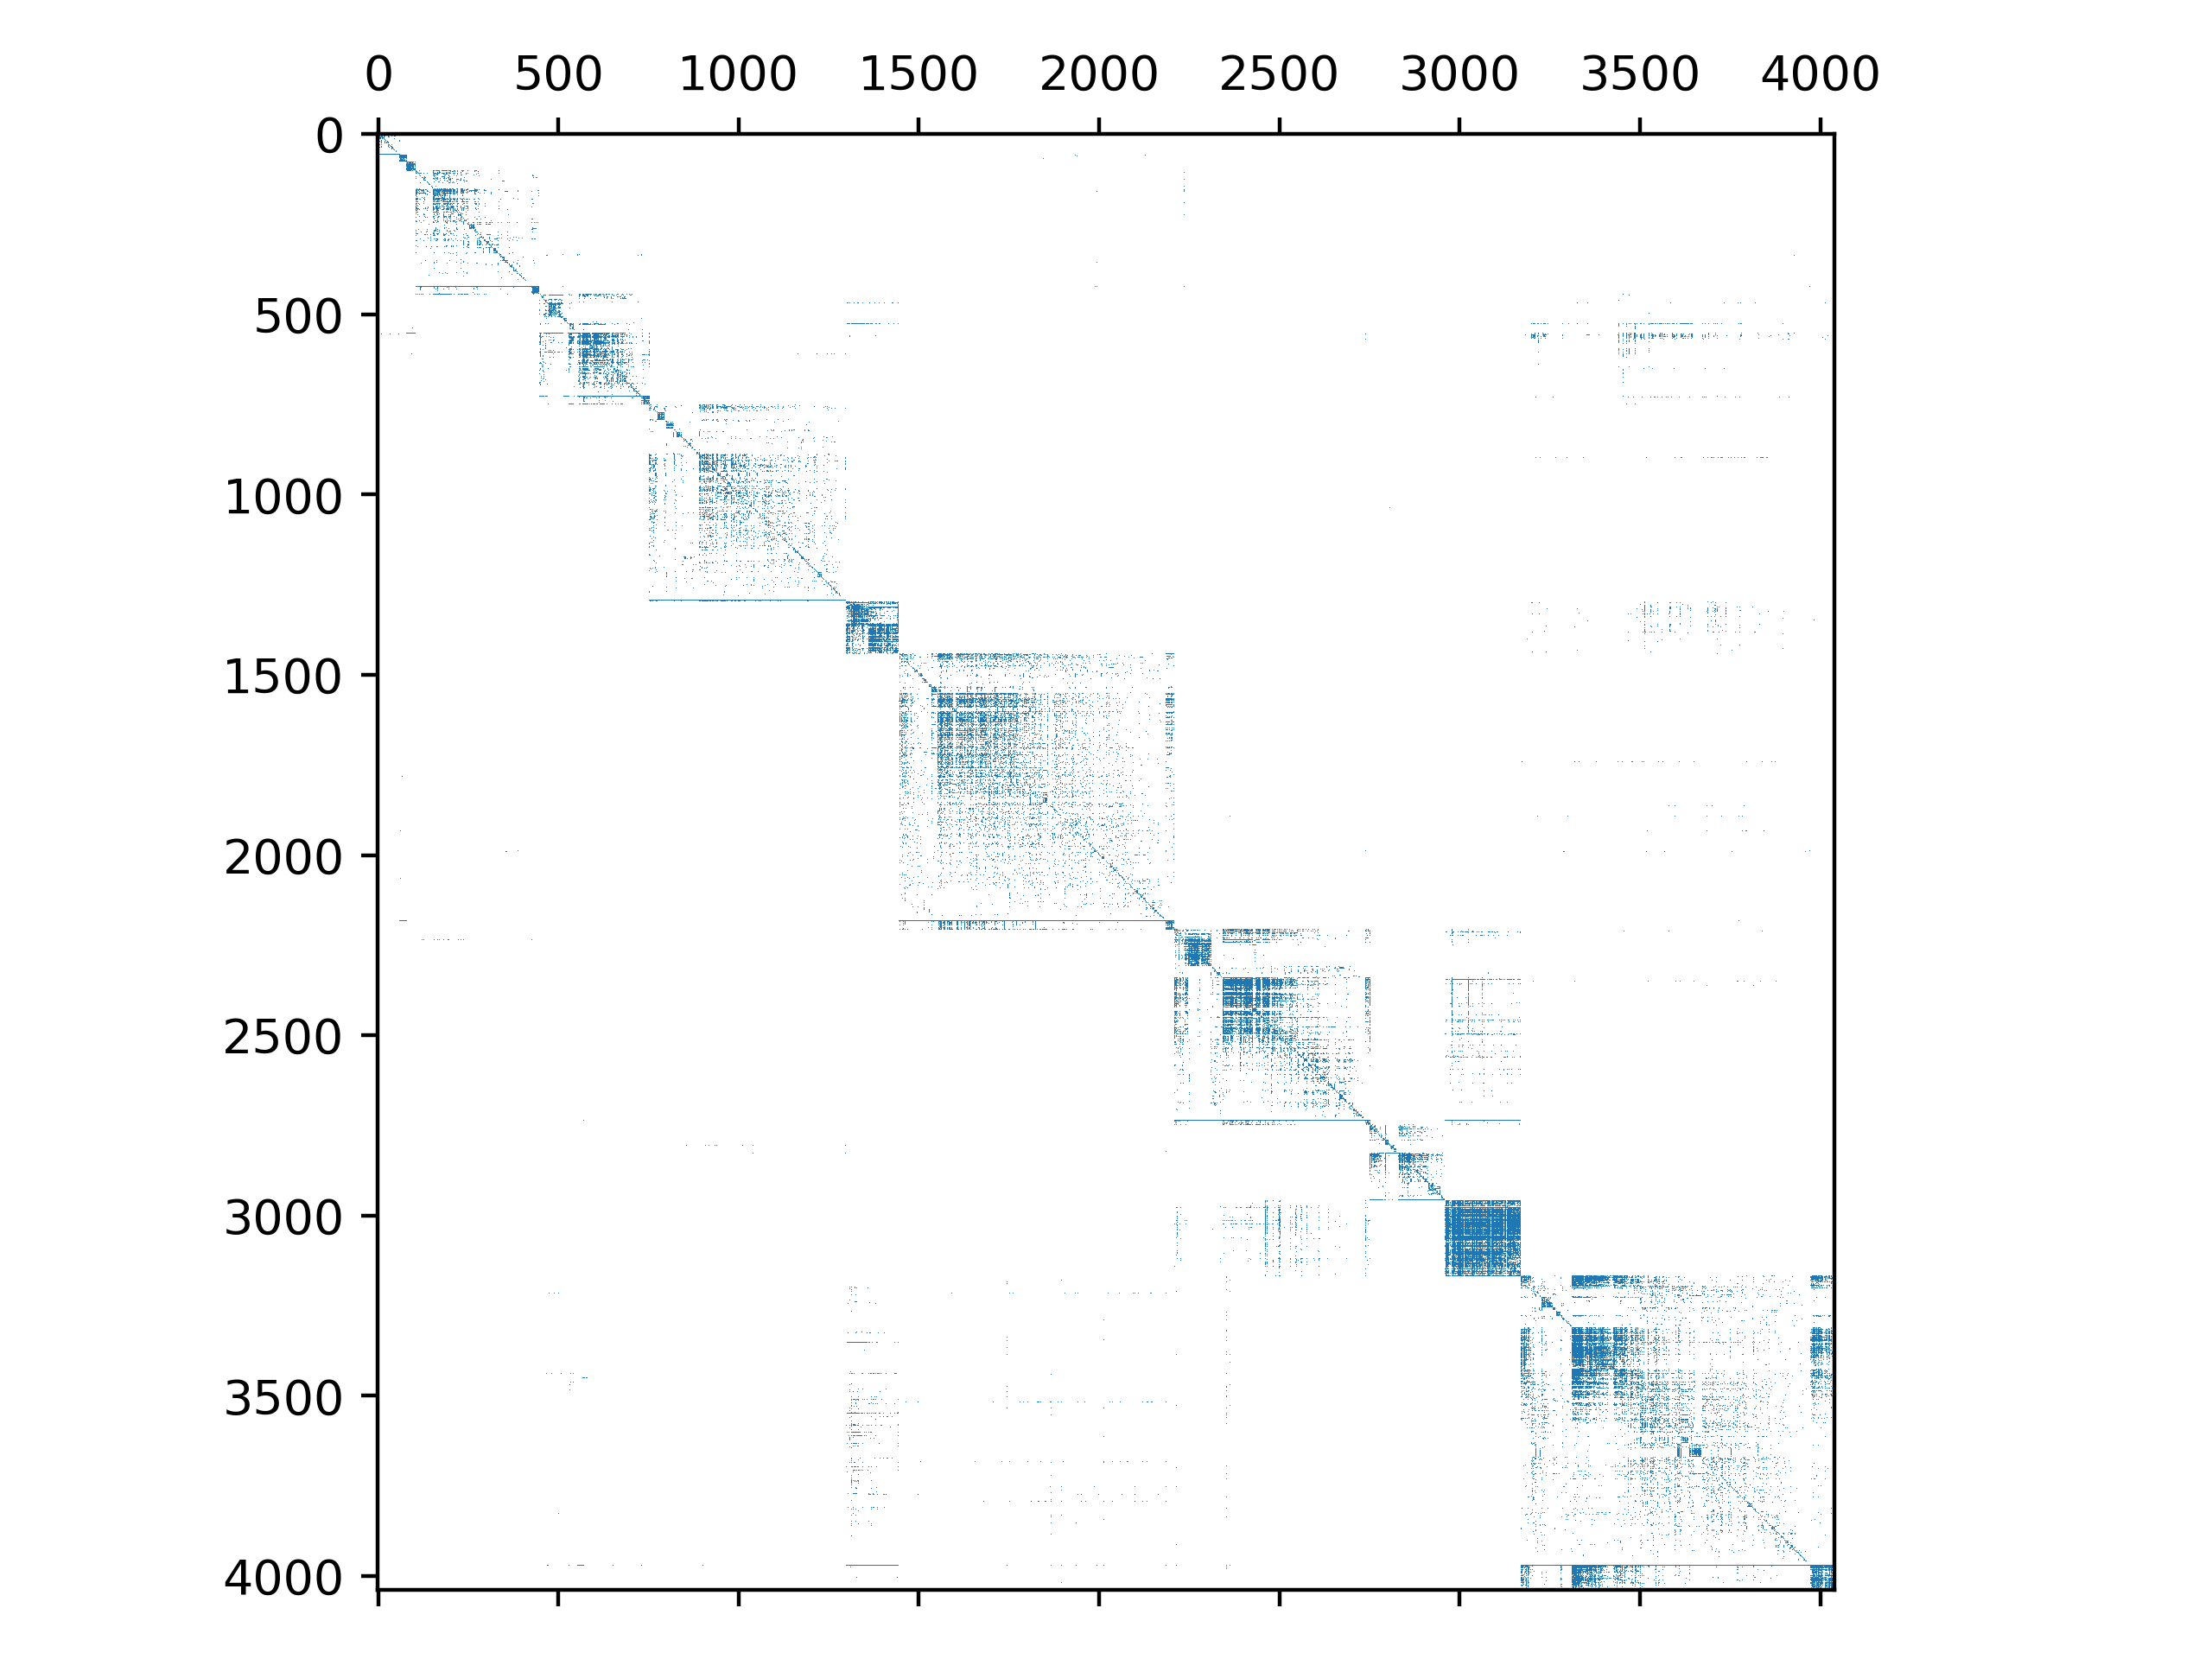
\includegraphics[width=5.5cm]{figures/fb-combined-rbt.png}}\hfil
  \subfloat[Cuthill-McKee Order]{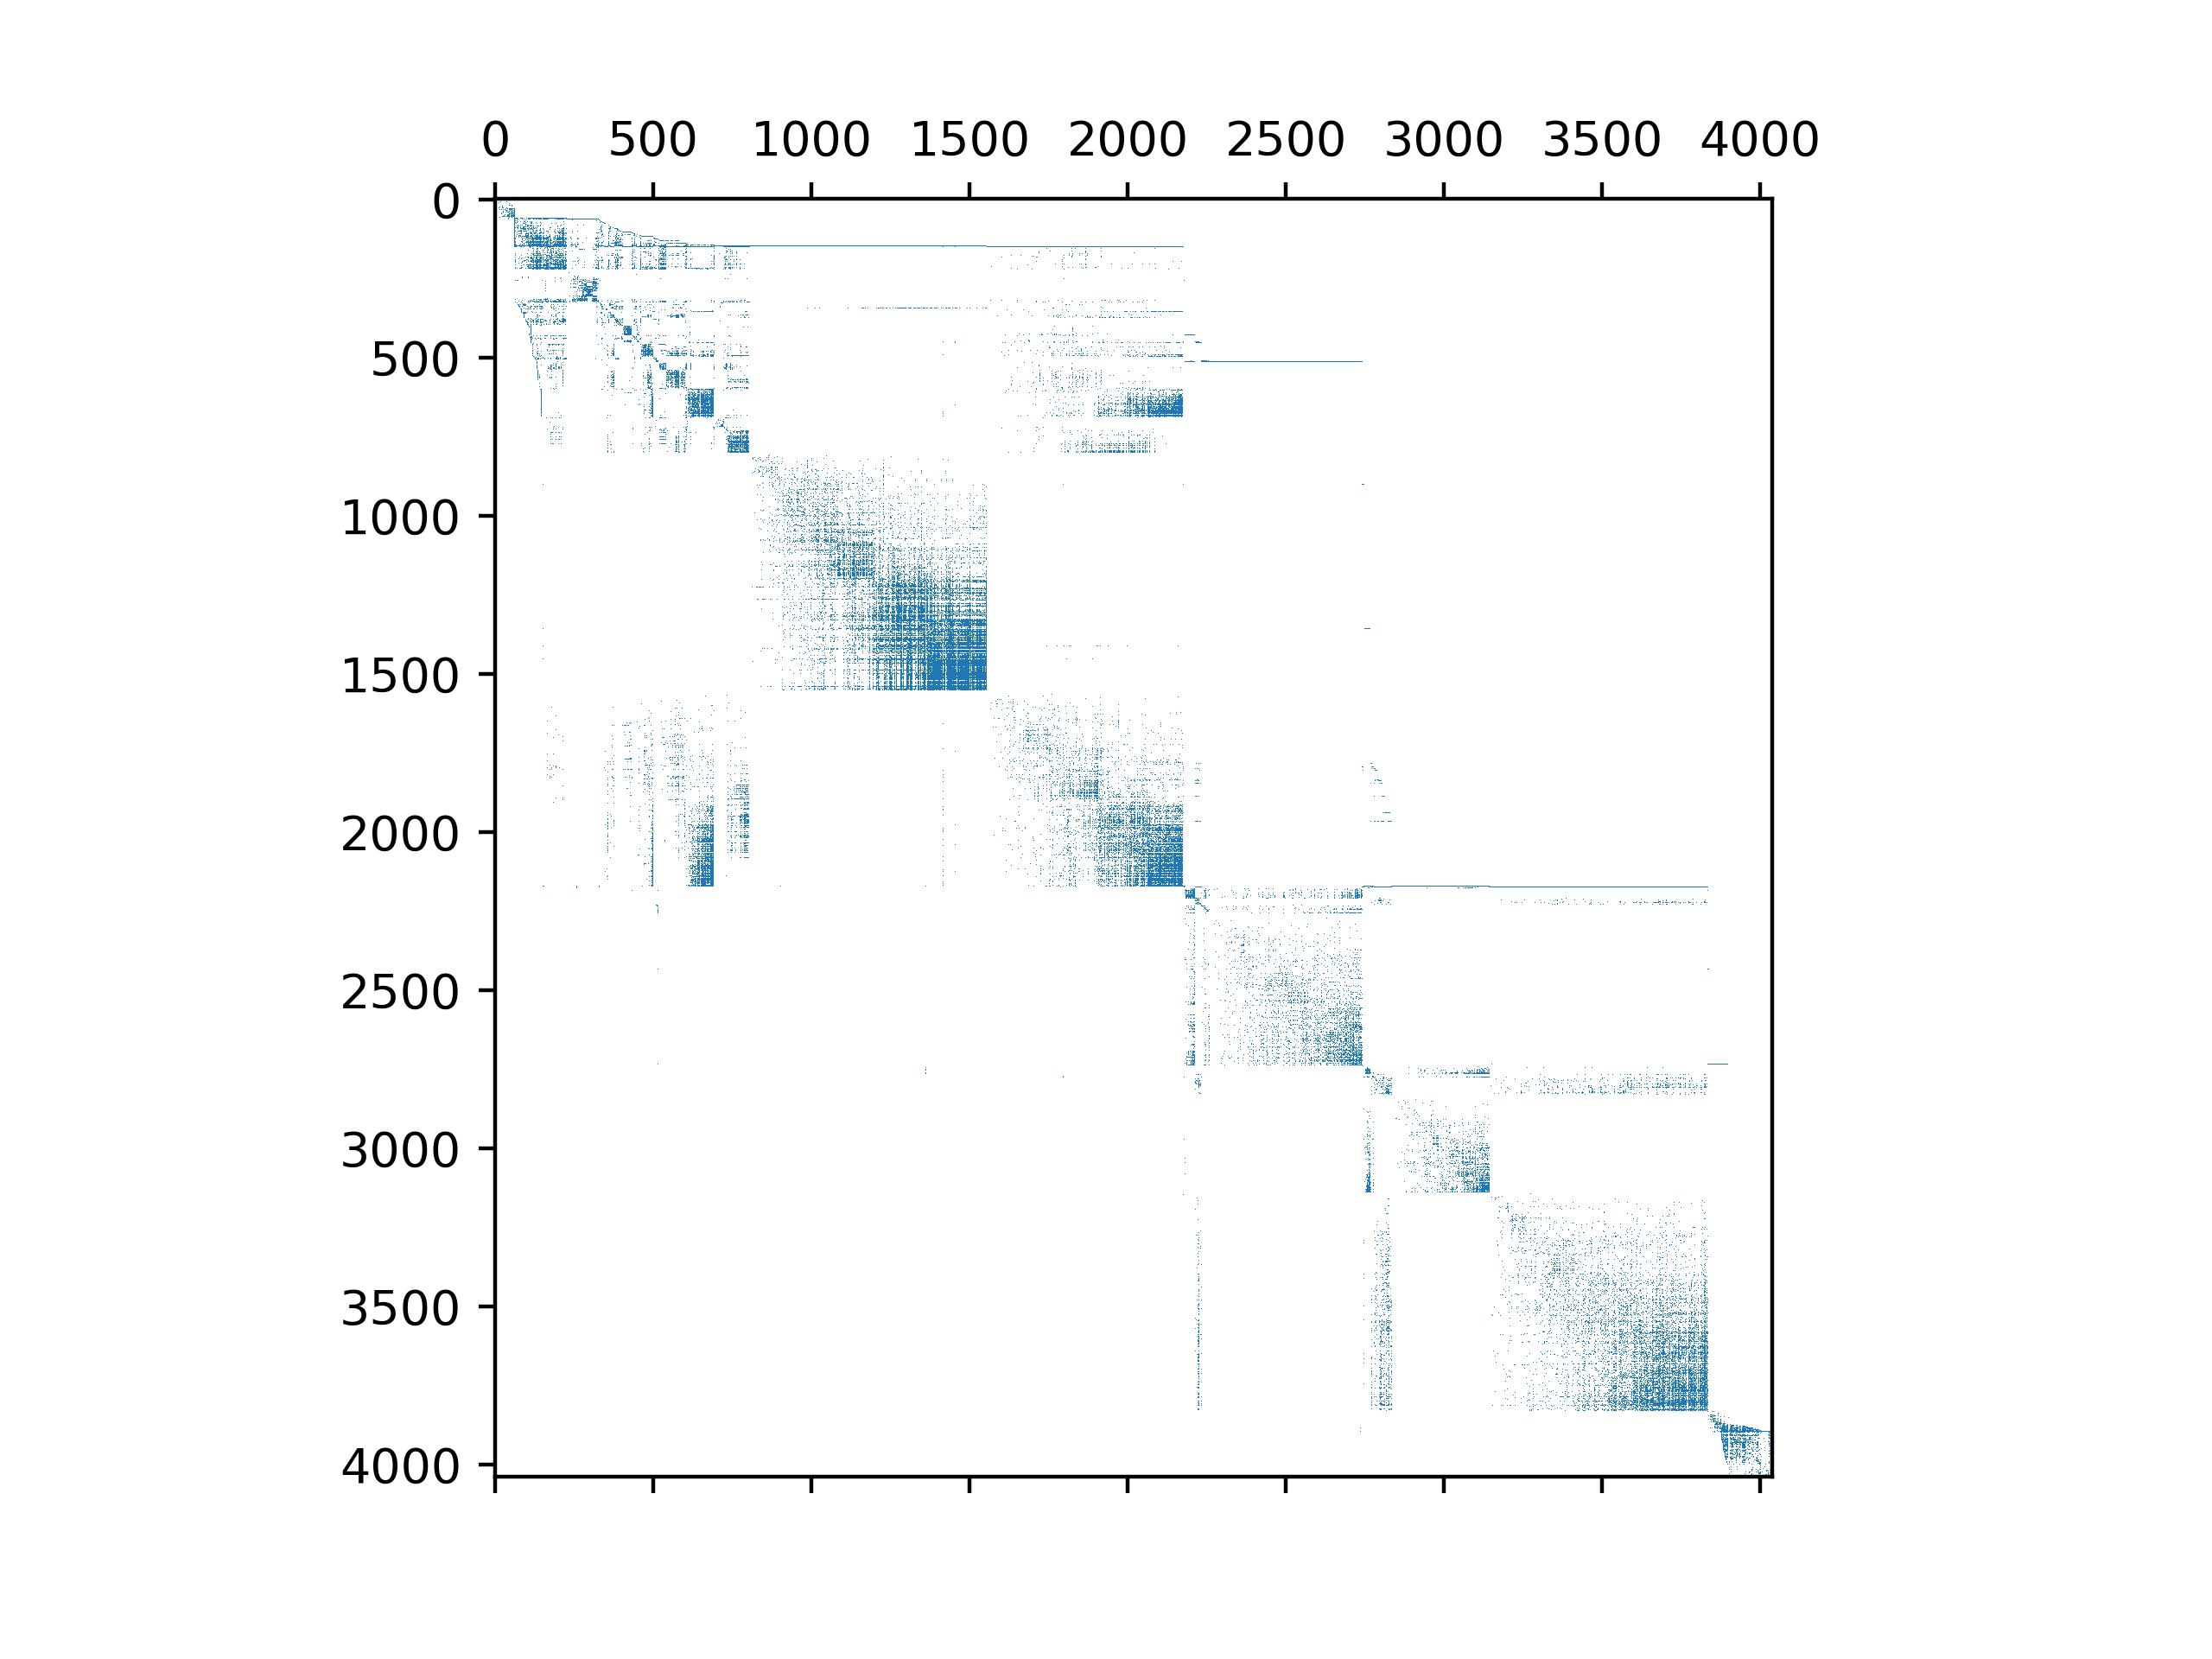
\includegraphics[width=5.5cm]{figures/fb-combined-rcm.png}}
  \caption{Adjacency matrices of an undirected Facebook Social Network graph with 4,039 vertices and 88,234 edges. Each pixel denotes an undirected edge (``friend-of'' relationship) between a pair of vertices (users) in the graph. Note the detected dense communities (submatrices) along the diagonal in (b) and the reduced bandwidth of the sparse matrix in (c). }\label{fig:fb_adjmats1}
  \end{figure*}

To date, researchers have looked at \textit{either} vertex or edge ordering to optimize the performance of their \ac{VC} or \ac{EC} systems, but there has not been an extensive evaluation of possible \textit{vertex-and-edge} orderings. We define a \textbf{Vertex-and-Edge Ordering} of a graph as a preprocessing algorithm that:
\begin{enumerate}
    \item Reorders the \textit{vertices} to introduce structure into the adjacency matrix.
    \item Traverses the \textit{edges} using an edge ordering that leverages the structure of the isomorphic adjacency matrix. For example, the edge ordering could skip over large empty regions and traverse the dense regions using the \ac{HSFC}.
\end{enumerate}
This thesis is concerned in filling this knowledge gap and investigates the interaction between Vertex and Edge ordering. Namely, we answer the following research questions:

\textbf{RQ1}: It has been shown that vertex and edge ordering confer performance benefits in a variety of applications. Is it possible to combine vertex
and edge ordering as a preprocessing step such that the performance benefit gained by the combination of both is compounded (i.e., is greater than using either separately)?
\begin{itemize}
  \item Can edge-centric graph traversal be sped up by first introducing some structure into the adjacency matrix?
\end{itemize}

\textbf{RQ2}: Given an arbitrary input graph, is there a \textit{vertex-and-edge} ordering combination that yields the best performance for an \ac{EC} traversal (measured in speed of execution and number of cache misses)?

We answer these questions by making the following contributions. We:

\begin{enumerate}
  \item {Perform a preliminary performance evaluation on different vertex and edge orderings on single-threaded \ac{EC} traversals for a variety of graph datasets. We conclude that there \textit{does not} exist a one-size-fits-all \textit{vertex-and-edge} ordering that outperforms all others for all types of graphs.}
  \item {Derive an analytic model of performance using a dataset of graph features (statistical measures that summarize a graph) to identify the characteristics of a graph that help us determine which vertex-and-edge ordering performs best for \ac{EC} workloads.}
  \item {Develop a fully parallel implementation of the SlashBurn vertex ordering technique: \textbf{ParSB}.}
  \item {Propose a novel, lock-free, multithreaded vertex-and-edge ordering technique that leverages the compressed graph representation given by ParSB and traverses the edges of the graph using the \ac{HSFC}.}
  \item {Evaluate our novel vertex-and-edge ordering and compare its performance against locking-based and merging-based multithreaded vertex-and-edge orderings.}
\end{enumerate}

$<$here would be an outline of the thesis, detailing the sections of it, and what each section contains.$>$

\begin{enumerate}[label*=\arabic*.]
  \item {\textbf{Introduction}}
  \item {
    
    
  }
  \item {\textbf{Case Study: Does Vertex-and-Edge ordering affect performance?}
  To answer \textbf{RQ1}, we ran the following experiment on a dataset of $\approx 150$ graphs whose size ranges from modest ($\approx$30MB) to large ($\approx$40GB). For each graph, we computed 8 vertex orderings. For each vertex ordering, we completed 20 iterations of PageRank using either Row-major, Column-major, or the Hilbert Order. We saw that there was not a 1-size-fits-all vertex-and-edge ordering combination.
  Highlight the different results observed. Visualize dataset of graphs in (reduced) high-dimensional space (t-SNE, PCA) to try to identify clusters of graphs that behave similarly. Present a simple, interpretable model (decision tree, linear regression) that identifies the features that influence the performance of different vertex-and-edge orders.  
  }
  

  \item {\textbf{Parallel Slashburn}
  The results of the case study show that, for certain graphs, SlashBurn produced the greatest performance improvements. Motivated by this, we propose to parallelize this algorithm, to speedup the computation of this ordering 
  % (thereby producing a "somewhat-lightweight" vertex reordering.)
  Describe the SlashBurn algorithm in depth. Highlight subroutines of the algorithm that are parallelizable. Describe the Parallel Slashburn algorithm. Evaluate:
  \begin{itemize}
    \item The speedup between the sequential and parallel implementation.
    \item Scalability: speedup when increasing the number of threads.
    \item Equality of results: the orderings produced by the sequential and parallel implementations should be almost identical. 
    Show that this is the case by measuring the performance improvement that is gained by both implementations, and show how these improvements are practically identical.
  \end{itemize}
  }
  \begin{enumerate}[label*=\arabic*.]
    \item {\textbf{Modelling the \ac{WWR} of Real-world Graph}
    Define the \ac{WWR} of a graph: the number of iterations to compute the slashburn ordering $\times$ the number of hubs selected at each SlashBurn iteration.
    Note the differences in the \ac{WWR} among graphs. Observe that this metric is a deciding factor of whether to use the SlashBurn order or not. 
    Model the \ac{WWR} as a function of graph features. Use our model of \ac{WWR} to predict whether to iterate over the graph using our proposed HilBurn curve.
    }
  \end{enumerate}
  \item {\textbf{My Technique: Vertex-and-Edge Ordering using HilBurn}
    Given that we've seen combined speed ups using the combination of the SlashBurn Vertex Ordering and the Hilbert Edge Ordering, We propose the Hilbert+SlashBurn Vertex-and-Edge ordering, HilBurn.
    \begin{enumerate}
      \item First, reorder the vertices of the graph using the ordering produced by Parallel SlashBurn. 
      \begin{itemize}
      \item Use the analytic model that predicts the \ac{WWR} of a graph given its graph statistics to choose the number of hubs selected at each iteration. Use this model to optimize for a Wing Width that fits in the LLC.
      \item In the case where the \ac{WWR} is too large, we expect that HilBurn would not perform great, so use our model to pick an appropriate Vertex-and-Edge ordering based on the input graph's graph features. 
      \end{itemize}
      \item{
        Second, separate the reordered adjacency matrix into 4 ``zones'':
        \begin{enumerate}
          \item {
            \textbf{Upper Right Quadrant - URQ}: this region should fit in the LLC. This range is defined by: $[0, ki)$, where:
            \begin{itemize}
              \item  $k$ is the number of hubs selected at each Parallel Slashburn iteration
              \item  $i$ is the number of iterations it took to complete Parallel Slashburn
            \end{itemize}
            The URQ will be computed in parallel by splitting up the $ki \times ki$ quadrant of the adjacency matrix into subquadrants, each of which contains a copy of the vertex ids in the range of its subquadrant to ensure
            that no contention occurs while updating vertex data.
            At the end of each iteration, all threads merge the updates for the vertices in their subquadrants;
          }
          \item{\textbf{Right Wing}:
          Can be computed in parallel with URQ. The upper right wing will be split into quadrants based on the number of edges in each region - this is done to ensure a workload balance among the threads operating on the right wing.
          Each thread will own a non-overlapping region of the vertex id range: $[ki, N-1)$. No locks or merging required for this step.
          }
          \item{\textbf{Left Wing}:
          
          }
          \item{\textbf{Tail}}
        \end{enumerate}
      }
      
    \end{enumerate}
  }
  \item {\textbf{Evaluation}}
  \item {\textbf{Discussion}}
  \item {\textbf{Future Work}}
  \item \begin{enumerate}[label*=\arabic*.]
    \item {\textbf{SIMD Parallelism}}
    \item {\textbf{Further speedups using other state of the art (PQ, CCs, degree sorts)}}
  \end{enumerate}
  \item {\textbf{Conclusion}}

\end{enumerate}

% This document provides a quick set of instructions for using the
% \class{ubcdiss} class to write a dissertation in \LaTeX. 
% Unfortunately this document cannot provide an introduction to using
% \LaTeX.  The classic reference for learning \LaTeX\ is
% \citeauthor{lamport-1994-ladps}'s
% book~\cite{lamport-1994-ladps}.  There are also many freely-available
% tutorials online;
% \webref{http://www.andy-roberts.net/misc/latex/}{Andy Roberts' online
%     \LaTeX\ tutorials}
% seems to be excellent.
% The source code for this docment, however, is intended to serve as
% an example for creating a \LaTeX\ version of your dissertation.

% We start by discussing organizational issues, such as splitting
% your dissertation into multiple files, in
% \autoref{sec:SuggestedThesisOrganization}.
% We then cover the ease of managing cross-references in \LaTeX\ in
% \autoref{sec:CrossReferences}.
% We cover managing and using bibliographies with \BibTeX\ in
% \autoref{sec:BibTeX}. 
% We briefly describe typesetting attractive tables in
% \autoref{sec:TypesettingTables}.
% We briefly describe including external figures in
% \autoref{sec:Graphics}, and using special characters and symbols
% in \autoref{sec:SpecialSymbols}.
% As it is often useful to track different versions of your dissertation,
% we discuss revision control further in
% \autoref{sec:DissertationRevisionControl}. 
% We conclude with pointers to additional sources of information in
% \autoref{sec:Conclusions}.

% %%%%%%%%%%%%%%%%%%%%%%%%%%%%%%%%%%%%%%%%%%%%%%%%%%%%%%%%%%%%%%%%%%%%%%
% \section{Suggested Thesis Organization}
% \label{sec:SuggestedThesisOrganization}

% The \acs{UBC} \acf{GPS} specifies a particular arrangement of the
% components forming a thesis.\footnote{See
%     \url{http://www.grad.ubc.ca/current-students/dissertation-thesis-preparation/order-components}}
% This template reflects that arrangement.

% In terms of writing your thesis, the recommended best practice for
% organizing large documents in \LaTeX\ is to place each chapter in
% a separate file.  These chapters are then included from the main
% file through the use of \verb+\include{file}+.  A thesis might
% be described as six files such as \file{intro.tex},
% \file{relwork.tex}, \file{model.tex}, \file{eval.tex},
% \file{discuss.tex}, and \file{concl.tex}.

% We also encourage you to use macros for separating how something
% will be typeset (\eg bold, or italics) from the meaning of that
% something. 
% For example, if you look at \file{intro.tex}, you will see repeated
% uses of a macro \verb+\file{}+ to indicate file names.
% The \verb+\file{}+ macro is defined in the file \file{macros.tex}.
% The consistent use of \verb+\file{}+ throughout the text not only
% indicates that the argument to the macro represents a file (providing
% meaning or semantics), but also allows easily changing how
% file names are typeset simply by changing the definition of the
% \verb+\file{}+ macro.
% \file{macros.tex} contains other useful macros for properly typesetting
% things like the proper uses of the latinate \emph{exempli grati\={a}}
% and \emph{id est} (\ie \verb+\eg+ and \verb+\ie+), 
% web references with a footnoted \acs{URL} (\verb+\webref{url}{text}+),
% as well as definitions specific to this documentation
% (\verb+\latexpackage{}+).

% %%%%%%%%%%%%%%%%%%%%%%%%%%%%%%%%%%%%%%%%%%%%%%%%%%%%%%%%%%%%%%%%%%%%%%
% \section{Making Cross-References}
% \label{sec:CrossReferences}

% \LaTeX\ make managing cross-references easy, and the \latexpackage{hyperref}
% package's\ \verb+\autoref{}+ command\footnote{%
%     The \latexpackage{hyperref} package is included by default in this
%     template.}
% makes it easier still. 

% A thing to be cross-referenced, such as a section, figure, or equation,
% is \emph{labelled} using a unique, user-provided identifier, defined
% using the \verb+\label{}+ command.  
% The thing is referenced elsewhere using the \verb+\autoref{}+ command.
% For example, this section was defined using:
% \begin{lstlisting}
%     \section{Making Cross-References}
%     \label{sec:CrossReferences}
% \end{lstlisting}
% References to this section are made as follows:
% \begin{lstlisting}
%     We then cover the ease of managing cross-references in \LaTeX\
%     in \autoref{sec:CrossReferences}.
% \end{lstlisting}
% \verb+\autoref{}+ takes care of determining the \emph{type} of the 
% thing being referenced, so the example above is rendered as
% \begin{quote}
%     We then cover the ease of managing cross-references in \LaTeX\
%     in \autoref{sec:CrossReferences}.
% \end{quote}

% The label is any simple sequence of characters, numbers, digits,
% and some punctuation marks such as ``:'' and ``--''; there should
% be no spaces.  Try to use a consistent key format: this simplifies
% remembering how to make references.  This document uses a prefix
% to indicate the type of the thing being referenced, such as \texttt{sec}
% for sections, \texttt{fig} for figures, \texttt{tbl} for tables,
% and \texttt{eqn} for equations.

% For details on defining the text used to describe the type
% of \emph{thing}, search \file{diss.tex} and the \latexpackage{hyperref}
% documentation for \texttt{autorefname}.


% %%%%%%%%%%%%%%%%%%%%%%%%%%%%%%%%%%%%%%%%%%%%%%%%%%%%%%%%%%%%%%%%%%%%%%
% \section{Managing Bibliographies with \BibTeX}
% \label{sec:BibTeX}

% One of the primary benefits of using \LaTeX\ is its companion program,
% \BibTeX, for managing bibliographies and citations.  Managing
% bibliographies has three parts: (i) describing references,
% (ii)~citing references, and (iii)~formatting cited references.

% \subsection{Describing References}

% \BibTeX\ defines a standard format for recording details about a
% reference.  These references are recorded in a file with a
% \file{.bib} extension.  \BibTeX\ supports a broad range of
% references, such as books, articles, items in a conference proceedings,
% chapters, technical reports, manuals, dissertations, and unpublished
% manuscripts. 
% A reference may include attributes such as the authors,
% the title, the page numbers, the \ac{DOI}, or a \ac{URL}.  A reference
% can also be augmented with personal attributes, such as a rating,
% notes, or keywords.

% Each reference must be described by a unique \emph{key}.\footnote{%
%     Note that the citation keys are different from the reference
%     identifiers as described in \autoref{sec:CrossReferences}.}
% A key is a simple sequence of characters, numbers, digits, and some
% punctuation marks such as ``:'' and ``--''; there should be no spaces. 
% A consistent key format simiplifies remembering how to make references. 
% For example:
% \begin{quote}
%    \fbox{\emph{last-name}}\texttt{-}\fbox{\emph{year}}\texttt{-}\fbox{\emph{contracted-title}}
% \end{quote}
% where \emph{last-name} represents the last name for the first author,
% and \emph{contracted-title} is some meaningful contraction of the
% title.  Then \citeauthor{kiczales-1997-aop}'s seminal article on
% aspect-oriented programming~\cite{kiczales-1997-aop} (published in
% \citeyear{kiczales-1997-aop}) might be given the key
% \texttt{kiczales-1997-aop}.

% An example of a \BibTeX\ \file{.bib} file is included as
% \file{biblio.bib}.  A description of the format a \file{.bib}
% file is beyond the scope of this document.  We instead encourage
% you to use one of the several reference managers that support the
% \BibTeX\ format such as
% \webref{http://jabref.sourceforge.net}{JabRef} (multiple platforms) or
% \webref{http://bibdesk.sourceforge.net}{BibDesk} (MacOS\,X only). 
% These front ends are similar to reference managers such as
% EndNote or RefWorks.


% \subsection{Citing References}

% Having described some references, we then need to cite them.  We
% do this using a form of the \verb+\cite+ command.  For example:
% \begin{lstlisting}
%     \citet{kiczales-1997-aop} present examples of crosscutting 
%     from programs written in several languages.
% \end{lstlisting}
% When processed, the \verb+\citet+ will cause the paper's authors
% and a standardized reference to the paper to be inserted in the
% document, and will also include a formatted citation for the paper
% in the bibliography.  For example:
% \begin{quote}
%     \citet{kiczales-1997-aop} present examples of crosscutting 
%     from programs written in several languages.
% \end{quote}
% There are several forms of the \verb+\cite+ command (provided
% by the \latexpackage{natbib} package), as demonstrated in
% \autoref{tbl:natbib:cite}.
% Note that the form of the citation (numeric or author-year) depends
% on the bibliography style (described in the next section).
% The \verb+\citet+ variant is used when the author names form
% an object in the sentence, whereas the \verb+\citep+ variant
% is used for parenthetic references, more like an end-note.
% Use \verb+\nocite+ to include a citation in the bibliography
% but without an actual reference.
% \nocite{rowling-1997-hpps}
% \begin{table}
% \caption{Available \texttt{cite} variants; the exact citation style
%     depends on whether the bibliography style is numeric or author-year.}
% \label{tbl:natbib:cite}
% \centering
% \begin{tabular}{lp{3.25in}}\toprule
% Variant & Result \\
% \midrule
% % We cheat here to simulate the cite/citep/citet for APA-like styles
% \verb+\cite+ & Parenthetical citation (\eg ``\cite{kiczales-1997-aop}''
%     or ``(\citeauthor{kiczales-1997-aop} \citeyear{kiczales-1997-aop})'') \\
% \verb+\citet+ & Textual citation: includes author (\eg
%     ``\citet{kiczales-1997-aop}'' or
%     or ``\citeauthor{kiczales-1997-aop} (\citeyear{kiczales-1997-aop})'') \\
% \verb+\citet*+ & Textual citation with unabbreviated author list \\
% \verb+\citealt+ & Like \verb+\citet+ but without parentheses \\
% \verb+\citep+ & Parenthetical citation (\eg ``\cite{kiczales-1997-aop}''
%     or ``(\citeauthor{kiczales-1997-aop} \citeyear{kiczales-1997-aop})'') \\
% \verb+\citep*+ & Parenthetical citation with unabbreviated author list \\
% \verb+\citealp+ & Like \verb+\citep+ but without parentheses \\
% \verb+\citeauthor+ & Author only (\eg ``\citeauthor{kiczales-1997-aop}'') \\
% \verb+\citeauthor*+ & Unabbreviated authors list 
%     (\eg ``\citeauthor*{kiczales-1997-aop}'') \\
% \verb+\citeyear+ & Year of citation (\eg ``\citeyear{kiczales-1997-aop}'') \\
% \bottomrule
% \end{tabular}
% \end{table}

% \subsection{Formatting Cited References}

% \BibTeX\ separates the citing of a reference from how the cited
% reference is formatted for a bibliography, specified with the
% \verb+\bibliographystyle+ command. 
% There are many varieties, such as \texttt{plainnat}, \texttt{abbrvnat},
% \texttt{unsrtnat}, and \texttt{vancouver}.
% This document was formatted with \texttt{abbrvnat}.
% Look through your \TeX\ distribution for \file{.bst} files. 
% Note that use of some \file{.bst} files do not emit all the information
% necessary to properly use \verb+\citet{}+, \verb+\citep{}+,
% \verb+\citeyear{}+, and \verb+\citeauthor{}+.

% There are also packages available to place citations on a per-chapter
% basis (\latexpackage{bibunits}), as footnotes (\latexpackage{footbib}),
% and inline (\latexpackage{bibentry}).
% Those who wish to exert maximum control over their bibliography
% style should see the amazing \latexpackage{custom-bib} package.

% %%%%%%%%%%%%%%%%%%%%%%%%%%%%%%%%%%%%%%%%%%%%%%%%%%%%%%%%%%%%%%%%%%%%%%
% \section{Typesetting Tables}
% \label{sec:TypesettingTables}

% \citet{lamport-1994-ladps} made one grievous mistake
% in \LaTeX: his suggested manner for typesetting tables produces
% typographic abominations.  These suggestions have unfortunately
% been replicated in most \LaTeX\ tutorials.  These
% abominations are easily avoided simply by ignoring his examples
% illustrating the use of horizontal and vertical rules (specifically
% the use of \verb+\hline+ and \verb+|+) and using the
% \latexpackage{booktabs} package instead.

% The \latexpackage{booktabs} package helps produce tables in the form
% used by most professionally-edited journals through the use of
% three new types of dividing lines, or \emph{rules}.
% % There are times that you don't want to use \autoref{}
% Tables~\ref{tbl:natbib:cite} and~\ref{tbl:LaTeX:Symbols} are two
% examples of tables typeset with the \latexpackage{booktabs} package.
% The \latexpackage{booktabs} package provides three new commands
% for producing rules:
% \verb+\toprule+ for the rule to appear at the top of the table,
% \verb+\midrule+ for the middle rule following the table header,
% and \verb+\bottomrule+ for the bottom-most at the end of the table.
% These rules differ by their weight (thickness) and the spacing before
% and after.
% A table is typeset in the following manner:
% \begin{lstlisting}
%     \begin{table}
%     \caption{The caption for the table}
%     \label{tbl:label}
%     \centering
%     \begin{tabular}{cc}
%     \toprule
%     Header & Elements \\
%     \midrule
%     Row 1 & Row 1 \\
%     Row 2 & Row 2 \\
%     % ... and on and on ...
%     Row N & Row N \\
%     \bottomrule
%     \end{tabular}
%     \end{table}
% \end{lstlisting}
% See the \latexpackage{booktabs} documentation for advice in dealing with
% special cases, such as subheading rules, introducing extra space
% for divisions, and interior rules.

% %%%%%%%%%%%%%%%%%%%%%%%%%%%%%%%%%%%%%%%%%%%%%%%%%%%%%%%%%%%%%%%%%%%%%%
% \section{Figures, Graphics, and Special Characters}
% \label{sec:Graphics}

% Most \LaTeX\ beginners find figures to be one of the more challenging
% topics.  In \LaTeX, a figure is a \emph{floating element}, to be
% placed where it best fits.
% The user is not expected to concern him/herself with the placement
% of the figure.  The figure should instead be labelled, and where
% the figure is used, the text should use \verb+\autoref+ to reference
% the figure's label.
% \autoref{fig:latex-affirmation} is an example of a figure.
% \begin{figure}
%     \centering
%     % For the sake of this example, we'll just use text
%     %\includegraphics[width=3in]{file}
%     \Huge{\textsf{\LaTeX\ Rocks!}}
%     \caption{Proof of \LaTeX's amazing abilities}
%     \label{fig:latex-affirmation}   % label should change
% \end{figure}
% A figure is generally included as follows:
% \begin{lstlisting}
%     \begin{figure}
%     \centering
%     \includegraphics[width=3in]{file}
%     \caption{A useful caption}
%     \label{fig:fig-label}   % label should change
%     \end{figure}
% \end{lstlisting}
% There are three items of note:
% \begin{enumerate}
% \item External files are included using the \verb+\includegraphics+
%     command.  This command is defined by the \latexpackage{graphicx} package
%     and can often natively import graphics from a variety of formats.
%     The set of formats supported depends on your \TeX\ command processor.
%     Both \texttt{pdflatex} and \texttt{xelatex}, for example, can
%     import \textsc{gif}, \textsc{jpg}, and \textsc{pdf}.  The plain
%     version of \texttt{latex} only supports \textsc{eps} files.

% \item The \verb+\caption+ provides a caption to the figure. 
%     This caption is normally listed in the List of Figures; you
%     can provide an alternative caption for the LoF by providing
%     an optional argument to the \verb+\caption+ like so:
%     \begin{lstlisting}
%     \caption[nice shortened caption for LoF]{%
% 	longer detailed caption used for the figure}
%     \end{lstlisting}
%     \ac{GPS} generally prefers shortened single-line captions
%     in the LoF: multiple-line captions are a bit unwieldy.

% \item The \verb+\label+ command provides for associating a unique, user-defined,
%     and descriptive identifier to the figure.  The figure can be
%     can be referenced elsewhere in the text with this identifier
%     as described in \autoref{sec:CrossReferences}.
% \end{enumerate}
% See Keith Reckdahl’s excellent guide for more details,
% \webref{http://www.ctan.org/tex-archive/info/epslatex.pdf}{\emph{Using
% imported graphics in LaTeX2e}}.

% \section{Special Characters and Symbols}
% \label{sec:SpecialSymbols}

% \LaTeX\ appropriates many common symbols for its own purposes,
% with some used for commands (\eg \verb+\{}&%+) and
% mathematics (\eg \verb+$^_+), and others are automagically transformed
% into typographically-preferred forms (\eg \verb+-`'+) or to
% completely different forms (\eg \verb+<>+).
% \autoref{tbl:LaTeX:Symbols} presents a list of common symbols and
% their corresponding \LaTeX\ commands.  A much more comprehensive list 
% of symbols and accented characters is available at:
% \url{http://www.ctan.org/tex-archive/info/symbols/comprehensive/}
% \begin{table}
% \caption{Useful \LaTeX\ symbols}\label{tbl:LaTeX:Symbols}
% \centering\begin{tabular}{ccp{0.5cm}cc}\toprule
% \LaTeX & Result && \LaTeX & Result \\
% \midrule
%     \verb+\texttrademark+ & \texttrademark && \verb+\&+ & \& \\
%     \verb+\textcopyright+ & \textcopyright && \verb+\{ \}+ & \{ \} \\
%     \verb+\textregistered+ & \textregistered && \verb+\%+ & \% \\
%     \verb+\textsection+ & \textsection && \verb+\verb!~!+ & \verb!~! \\
%     \verb+\textdagger+ & \textdagger && \verb+\$+ & \$ \\
%     \verb+\textdaggerdbl+ & \textdaggerdbl && \verb+\^{}+ & \^{} \\
%     \verb+\textless+ & \textless && \verb+\_+ & \_ \\
%     \verb+\textgreater+ & \textgreater && \\
% \bottomrule
% \end{tabular}
% \end{table}

% %%%%%%%%%%%%%%%%%%%%%%%%%%%%%%%%%%%%%%%%%%%%%%%%%%%%%%%%%%%%%%%%%%%%%%
% \section{Changing Page Widths and Heights}

% The \class{ubcdiss} class is based on the standard \LaTeX\ \class{book}
% class~\cite{lamport-1994-ladps} that selects a line-width to carry
% approximately 66~characters per line.  This character density is
% claimed to have a pleasing appearance and also supports more rapid
% reading~\cite{bringhurst-2002-teots}.  I would recommend that you
% not change the line-widths!

% \subsection{The \texttt{geometry} Package}

% Some students are unfortunately saddled with misguided supervisors
% or committee members whom believe that documents should have the
% narrowest margins possible.  The \latexpackage{geometry} package is
% helpful in such cases.  Using this package is as simple as:
% \begin{lstlisting}
%     \usepackage[margin=1.25in,top=1.25in,bottom=1.25in]{geometry}
% \end{lstlisting}
% You should check the package's documentation for more complex uses.

% \subsection{Changing Page Layout Values By Hand}

% There are some miserable students with requirements for page layouts
% that vary throughout the document.  Unfortunately the
% \latexpackage{geometry} can only be specified once, in the document's
% preamble.  Such miserable students must set \LaTeX's layout parameters
% by hand:
% \begin{lstlisting}
%     \setlength{\topmargin}{-.75in}
%     \setlength{\headsep}{0.25in}
%     \setlength{\headheight}{15pt}
%     \setlength{\textheight}{9in}
%     \setlength{\footskip}{0.25in}
%     \setlength{\footheight}{15pt}

%     % The *sidemargin values are relative to 1in; so the following
%     % results in a 0.75 inch margin
%     \setlength{\oddsidemargin}{-0.25in}
%     \setlength{\evensidemargin}{-0.25in}
%     \setlength{\textwidth}{7in}       % 1.1in margins (8.5-2*0.75)
% \end{lstlisting}
% These settings necessarily require assuming a particular page height
% and width; in the above, the setting for \verb+\textwidth+ assumes
% a \textsc{US} Letter with an 8.5'' width.
% The \latexpackage{geometry} package simply uses the page height and
% other specified values to derive the other layout values.
% The
% \href{http://tug.ctan.org/tex-archive/macros/latex/required/tools/layout.pdf}{\texttt{layout}}
% package provides a
% handy \verb+\layout+ command to show the current page layout
% parameters. 


% \subsection{Making Temporary Changes to Page Layout}

% There are occasions where it becomes necessary to make temporary
% changes to the page width, such as to accomodate a larger formula. 
% The \latexmiscpackage{chngpage} package provides an \env{adjustwidth}
% environment that does just this.  For example:
% \begin{lstlisting}
%     % Expand left and right margins by 0.75in
%     \begin{adjustwidth}{-0.75in}{-0.75in}
%     % Must adjust the perceived column width for LaTeX to get with it.
%     \addtolength{\columnwidth}{1.5in}
%     \[ an extra long math formula \]
%     \end{adjustwidth}
% \end{lstlisting}


% %%%%%%%%%%%%%%%%%%%%%%%%%%%%%%%%%%%%%%%%%%%%%%%%%%%%%%%%%%%%%%%%%%%%%%
% \section{Keeping Track of Versions with Revision Control}
% \label{sec:DissertationRevisionControl}

% Software engineers have used \acf{RCS} to track changes to their
% software systems for decades.  These systems record the changes to
% the source code along with context as to why the change was required.
% These systems also support examining and reverting to particular
% revisions from their system's past.

% An \ac{RCS} can be used to keep track of changes to things other
% than source code, such as your dissertation.  For example, it can
% be useful to know exactly which revision of your dissertation was
% sent to a particular committee member.  Or to recover an accidentally
% deleted file, or a badly modified image.  With a revision control
% system, you can tag or annotate the revision of your dissertation
% that was sent to your committee, or when you incorporated changes
% from your supervisor.

% Unfortunately current revision control packages are not yet targetted
% to non-developers.  But the Subversion project's
% \webref{http://tortoisesvn.net/docs/release/TortoiseSVN_en/}{TortoiseSVN}
% has greatly simplified using the Subversion revision control system
% for Windows users.  You should consult your local geek.

% A simpler alternative strategy is to create a GoogleMail account
% and periodically mail yourself zipped copies of your dissertation.

% %%%%%%%%%%%%%%%%%%%%%%%%%%%%%%%%%%%%%%%%%%%%%%%%%%%%%%%%%%%%%%%%%%%%%%
% \section{Recommended Packages}

% The real strength to \LaTeX\ is found in the myriad of free add-on
% packages available for handling special formatting requirements.
% In this section we list some helpful packages.

% \subsection{Typesetting}

% \begin{description}
% \item[\latexpackage{enumitem}:]
%     Supports pausing and resuming enumerate environments.

% \item[\latexpackage{ulem}:]
%     Provides two new commands for striking out and crossing out text
%     (\verb+\sout{text}+ and \verb+\xout{text}+ respectively)
%     The package should likely
%     be used as follows:
%     \begin{verbatim}
%     \usepackage[normalem,normalbf]{ulem}
%     \end{verbatim}
%     to prevent the package from redefining the emphasis and bold fonts.

% \item[\latexpackage{chngpage}:]
%     Support changing the page widths on demand.

% \item[\latexpackage{mhchem}:] 
%     Support for typesetting chemical formulae and reaction equations.

% \end{description}

% Although not a package, the
% \webref{http://www.ctan.org/tex-archive/support/latexdiff/}{\texttt{latexdiff}}
% command is very useful for creating changebar'd versions of your
% dissertation.


% \subsection{Figures, Tables, and Document Extracts}

% \begin{description}
% \item[\latexpackage{pdfpages}:]
%     Insert pages from other PDF files.  Allows referencing the extracted
%     pages in the list of figures, adding labels to reference the page
%     from elsewhere, and add borders to the pages.

% \item[\latexpackage{subfig}:]
%     Provides for including subfigures within a figure, and includes
%     being able to separately reference the subfigures.  This is a
%     replacement for the older \texttt{subfigure} environment.

% \item[\latexpackage{rotating}:]
%     Provides two environments, sidewaystable and sidewaysfigure,
%     for typesetting tables and figures in landscape mode.  

% \item[\latexpackage{longtable}:]
%     Support for long tables that span multiple pages.

% \item[\latexpackage{tabularx}:]
%     Provides an enhanced tabular environment with auto-sizing columns.

% \item[\latexpackage{ragged2e}:]
%     Provides several new commands for setting ragged text (\eg forms
%     of centered or flushed text) that can be used in tabular
%     environments and that support hyphenation.

% \end{description}


% \subsection{Bibliography Related Packages}

% \begin{description}
% \item[\latexpackage{bibunits}:]
%     Support having per-chapter bibliographies.

% \item[\latexpackage{footbib}:]
%     Cause cited works to be rendered using footnotes.

% \item[\latexpackage{bibentry}:] 
%     Support placing the details of a cited work in-line.

% \item[\latexpackage{custom-bib}:]
%     Generate a custom style for your bibliography.

% \end{description}


% %%%%%%%%%%%%%%%%%%%%%%%%%%%%%%%%%%%%%%%%%%%%%%%%%%%%%%%%%%%%%%%%%%%%%%
% \section{Moving On}
% \label{sec:Conclusions}

% At this point, you should be ready to go.  Other handy web resources:
% \begin{itemize}
% \item \webref{http://www.ctan.org}{\ac{CTAN}} is \emph{the} comprehensive
%     archive site for all things related to \TeX\ and \LaTeX. 
%     Should you have some particular requirement, somebody else is
%     almost certainly to have had the same requirement before you,
%     and the solution will be found on \ac{CTAN}.  The links to
%     various packages in this document are all to \ac{CTAN}.

% \item An online
%     \webref{http://www.ctan.org/get/info/latex2e-help-texinfo/latex2e.html}{%
% 	reference to \LaTeX\ commands} provides a handy quick-reference
%     to the standard \LaTeX\ commands.

% \item The list of 
%     \webref{http://www.tex.ac.uk/cgi-bin/texfaq2html?label=interruptlist}{%
% 	Frequently Asked Questions about \TeX\ and \LaTeX}
%     can save you a huge amount of time in finding solutions to
%     common problems.

% \item The \webref{http://www.tug.org/tetex/tetex-texmfdist/doc/}{te\TeX\
%     documentation guide} features a very handy list of the most useful
%     packages for \LaTeX\ as found in \ac{CTAN}.

% \item The
% \webref{http://www.ctan.org/tex-archive/macros/latex/required/graphics/grfguide.pdf}{\texttt{color}}
%     package, part of the graphics bundle, provides handy commands
%     for changing text and background colours.  Simply changing
%     text to various levels of grey can have a very 
%     \textcolor{greytext}{dramatic effect}.


% \item If you're really keen, you might want to join the
%     \webref{http://www.tug.org}{\TeX\ Users Group}.

% \end{itemize}

\endinput

Any text after an \endinput is ignored.
You could put scraps here or things in progress.

% \chapter{Overview}
% \label{ch:Overview}

\textbf{Thesis Overview}

\begin{enumerate}
    \item{Introduction
    \begin{enumerate}[label*=\arabic*.]
        \item Fairy Tale, Contributions.
    \end{enumerate}
    }

    \item{Background}
    \begin{enumerate}[label*=\arabic*.]
        \item Notation
        \item In Memory Graph Data Structures
        \item{Graph Ordering}
        \begin{enumerate}[label*=\arabic*.]
            \item Memory Access Patterns and Bottlenecks in Graph Processing
            \item Vertex Reordering
            \item Edge Reordering
        \end{enumerate}
        \item{Modes of Graph Computation}
        \begin{enumerate}[label*=\arabic*.]
            \item Push vs. Pull
            \item Parallel Computation
            \begin{enumerate}[label*=\arabic*.]
                \item Propagation Blocking
            \end{enumerate}
    
        \end{enumerate}
    \end{enumerate}

    \item{Related Work}
    
    \item{Case Study: Single-threaded Vertex-and-Edge Ordering}
    \item{Case Study: Effect of Graph Fill (Density) on Hilbert Curve performance}
    
    \item{Parallel Slashburn}
    % \item{TAVERN - Topology-Aware Vertex-and-Edge Reordering eNhancement}
    \item{FAHR - Fill-Aware Hilbert Reordering }
    \item{Evaluation}
    \item{Discussion}
    \item{Future Work}
    \item{Conclusion}


    
        
\end{enumerate}

% \begin{enumerate}[label*=\arabic*.]
% \end{enumerate}



%    2. Main body
% Generally recommended to put each chapter into a separate file

\chapter{Background}
\label{ch:Background}

% In this chapter, we introduce and define common data structures that are used to represent graphs in memory.
% Our choice of in-memory graph data structure naturally leads into questions about how the graph's elements
% (vertices, edges) should be laid out, or ordered, within the constraints of the data structure we use to store them, which is the main focus of this thesis.

% We begin with Table \ref{tab:notation} which defines a common ground of 
% % conventional 
% symbols and constants that we 
% will 
% % continuously 
% refer to in this thesis. 
% We touch on the conventional data structures that have been used to represent graphs: \textbf{Adjacency List} and \textbf{Adjacency Matrix}, and how their inadequacies in representing large-scale, real-world, sparse graphs, has prompted the development of compressed graph representations: \ac{CSR} / \ac{CSC}. The widespread utilization of the \ac{CSR} as the de-facto data structure for in-memory \ac{GPS} has raised some important challenges, which \textit{graph ordering} has attempted to ameliorate and resolve.
% We define graph ordering, and specialize our definition by making the distinction between two common graph ordering methods: Vertex and Edge ordering
% %  and describe and categorize a selection of vertex and edge ordering techniques.
% We conclude this chapter with a discussion of different \textit{modes} of graph computation, and how the hurdles we describe in our introduction of the \ac{CSR} representation are further compounded in the parallel setting.

The focus of this thesis is how to \textit{layout}, or \textit{order}, a graph's elements and data in memory to speed up processing. So, we begin by introducing common data structures that are used to represent graphs in memory. 
% Once a data structure is selected, how we \textit{layout}, or \textit{order}, the graph's elements and data within the chosen data structure is the main focus of this thesis.
 We define our notation in Table \ref{tab:notation}. We review the conventional graph data structures: the Adjacency List and Adjacency Matrix, and show how they are inadequate for representing large-scale, real-world, sparse graphs. To address these limitations, compressed graph representations like \ac{CSR} and \ac{CSC} are used. 
% The \ac{CSR} has become the de-facto data structure for in-memory \ac{GPS}, but using it for graph analytics poses challenges that are further exacerbated in the parallel setting.
We introduce the different modes of parallel graph computation and illustrate the challenges that arise when using the \ac{CSR} representation for parallel graph processing. We conclude by defining \textit{graph ordering}, distinguising between two common methods: Vertex and Edge ordering, and showing how graph
ordering can address these challenges. 
\clearpage
% \section{Notation}
\setlength{\arrayrulewidth}{0.5mm}
\setlength{\tabcolsep}{18pt}
\renewcommand{\arraystretch}{1.5}

% \begin{lstlisting}
% Expand left and right margins by 0.75in
% Must adjust the perceived column width for LaTeX to get with it.
% \addtolength{\columnwidth}{1.5in}
% \[ an extra long math formula \]

\begin{table}
    \centering
    \begin{adjustwidth}{-0.75in}{-0.75in}

        \begin{tabular}{ |p{2cm}|p{6cm}|p{5cm}|  }
            % \hline
            % \multicolumn{3}{|c|}{Country List}                         \\
            \hline
            \textbf{Symbol}  & \textbf{Definition}                                                                                                 & \textbf{Notes}                \\
            \hline
            $V$              & Vertex Set                                                                                                          & -                             \\
            \hline
            $E$              & Edge Set                                                                                                            & -                             \\
            \hline

            $G(V, E)$        & A graph $G$, with vertex set $V$, and edge set $E$                                                                  & -                             \\
            \hline

            $G(V, E, w(E))$  & A weighted graph $G$, with vertex set $V$, edge set $E$, and a weight function $w: (V \times V) \mapsto \mathbb{R}$ & -                             \\
            \hline


            $B(V_1, V_2, E)$ & A bipartite graph $B$, with vertex sets $V_1, V_2$, and edge set $E$                                                & -                             \\
            \hline

            $n$              & The number of vertices in a graph                                                                                   & $|V|$                   \\
            \hline

            $m$              & The number of edges in a graph                                                                                      & $|E|$                   \\
            \hline

            $(u, v)$         & The edge between vertices $u, v$                                                                                    & May be directed or undirected \\
            \hline

            $A$              & The adjacency matrix of the directed graph, $G$                                                                     &                               \\
            \hline
            $n^{+/-}(u)$       & The out/in-neighbourhood of vertex $u$                                                                                 &                               \\
            \hline
            $n(u)$       & The neighbourhood of vertex $u$                                                                                  &                               \\
            \hline
            $deg^{+/-}(u)$     & The out/in-degree of vertex $u$ & $|n^{+}(u)|$/$|n^{-}(u)| $           \\
            \hline
            $deg(u)$     & The degree of vertex $u$   & $|n(u)|$            \\
            \hline
            $f(G)$     & The fill of a graph & $\frac{m}{n(n-1)}$            \\
            \hline
            $\overline{d}$ & The average degree of the graph & $\frac{m}{n}$            \\
            \hline
        \end{tabular}
        \caption{\label{tab:notation}Notation used in this thesis.}
    \end{adjustwidth}
\end{table}


% \end{lstlisting}


\section{In Memory Graph Data Structures}
% \par{
%     % We introduce ways to represent graphs in memory. We describe the conventional Adjacency matrix and 
%     % list representations of a graph, and how the vertices and edges of the graph are stored using 
%     % these data structures. Next, we introduce the commonly used, efficient   
%     % \ac{CSR}/\ac{CSC}
%     % graph representations, and illustrate challenges that arise from representing large graphs using these
%     % compressed representations. 
%     We introduce various methods for storing graphs in memory, including the traditional Adjacency Matrix and List representations. We explain how vertices and edges are stored using these data structures. We then present the efficient Compressed Sparse Row (CSR) and Compressed Sparse Column (CSC) representations commonly used for large graphs and highlight the challenges that arise when using these compressed representations.
% }


A graph $G(V, E)$ is an ordered pair of a vertex set, $V$, and an edge set $E$. Graphs may be directed and/or weighted. If a graph is directed, $E$ consists of \textit{ordered} pairs of vertices, whereas if $G$ is undirected, edges are \textit{unordered}.
$n$ is the number of vertices in the graph ($|V|$) and $m$ is the number of edges in the graph ($|E|$).
Given a directed graph and an edge $(u,v)$, we say that that $v$ is an \textit{out-neighbour} of $u$, $u$ is an in-neighbour of $v$, and that $u$ and $v$ are adjacent. In this thesis, we will assume graphs are directed.
If $G$ is a weighted graph, a weight function, $w: (V \times V) \mapsto \mathbb{R}$, maps each edge in the graph to a real value. A graph $B$ is said to be bipartite if $V$ can be decomposed into two disjoint vertex sets $V_1, V_2$, such that no two vertices within a vertex set are adjacent.
Figure \ref{fig:graph_example}a shows a directed graph, which we will use as a running example to show how the same graph is represented using either an Adjacency Matrix, Adjacency List, or the \ac{CSR} / \ac{CSC} representations.



% \caption{A Directed Graph $G(V, E)$ with \\$V=\{0,1,2,3,4,5,6,7\}$ and \\$E=\{
%         (0, 2),
%         (1, 5),
%         (1, 6),
%         (2, 0),
%         (2, 1),
%         (2, 4),
%         (2, 5),
%         (3, 2),
%         (3, 5),            
%         (4, 5),
%         (5, 2),
%         (5, 4),
%         (5, 6),
%         (6, 5)\}$ and its corresponding boolean, directed adjacency matrix, $A$}
\begin{figure}[!htb]
    \begin{adjustwidth}{-0.75in}{-0.75in}
        \centering
        \includesvg[width=6in]{./ipe_plots/in_mem_graph_structs.svg}
        \caption{
            In-memory Graph Representations
        }
        \label{fig:graph_example}   % label should change
    \end{adjustwidth}
\end{figure}


Many real world graphs derived from bioinformatics, social, or hyperlink networks are
\textit{scale-free} \cite{barabasi2009scale, sapco} and \textit{sparse} \cite{danisch2018listing}.
A graph is \textit{scale-free} if the degree distribution of its vertices follows a \textit{power-law}, where a small fraction of vertices make up a disproportionately large fraction of the edges of the graph. As such, the vertices of power-law graphs are typically labelled according to their degree. We follow the convention set out by \citet{esfahani2021locality}: the \textit{average degree} of the graph ($\overline{d}$) acts as the threshold between 
\textit{low-degree} and \textit{high-degree} vertices, and vertices whose degree is larger than $\sqrt{n}$ are called \textit{hub} vertices. 
A graph is \textit{sparse} if the number of edges in the graph is substantially smaller than the total number of possible edges (i.e., $m \ll n(n-1)$). 

A graph can be represented using an \textbf{Adjacency Matrix}, $A$ (Figure \ref{fig:graph_example}b), with $A_{i,j}$ corresponding to the edge $(i, j)$. If the graph is unweighted, $A$ is an $n\times n$ boolean matrix, with $A_{i,j} = 1$ indicating the existence of an edge $(i, j)$.
If the graph is weighted, the nonzero values of $A\in\mathbb{R}^{n\times n}$ correspond to the weight function, $w(E)$. The adjacency matrices of real world graphs are themselves, sparse matrices, with a majority of the entries in the matrix containing zero, or null, values. This has led researchers to frame graph processing in the form of matrix operations like \ac{SPMV} \cite{graphmat}. For example, the out- (in-) degrees of the vertices in the graph can be computed using the matrix-vector product: $A\mathbf{1}^T$ ($A^T\mathbf{1}^T$). However, representing real world graphs as sparse matrices is usually infeasible, due to the $O(n^2)$ memory footprint of the entire adjacency matrix.

Alternatively, a graph can be represented using an \textbf{Adjacency List} (Figure \ref{fig:graph_example}c), with the vertices of the graph stored in an array.
% where the vertices are sorted by their ascending Vertex ID. 
The neighbourhood of vertex $u$ (either $n^{+}(u)$ or $n^{-}(u)$ for the out- or in-neighbourhood of $u$) is usually stored in a linked list, and $u$'s neighbours are sorted by ascending Vertex ID. The memory requirements of the adjacency list ($O(n + m)$) are lesser than that of the adjacency matrix, which is particularly crucial when dealing with sparse graphs. However, the use of pointers to link vertex neighbourhoods raises an issue.
Graph algorithms typically rely on the repeated traversal of the neighbourhoods of vertices (e.g., \ac{BFS}, \ac{SSSP}). If the graph is stored using an adjacency list, this traversal will follow neighbouring pointers to iterate over the neighbourhood of each vertex. This raises difficulties for hardware prefetchers, since, assuming the neighbourhood linked list has not been seen in the past, a prefetcher cannot prefetch the data of the next vertex until we've loaded the neighbour pointer of the current vertex. This ``pointer-chasing'' issue hindering performance gains by hardware prefetching can be alleviated by laying out the neighbourhoods in a sorted, contiguous array.
%  which led to the de-facto in-memory graph data structure, the Compressed Sparse Row/Column (\ac{CSR}/\ac{CSC}).

The \textbf{Compressed Sparse Row/Column (\ac{CSR}/\ac{CSC})} representations (Figure \ref{fig:graph_example}d) achieve this data layout by using two arrays to store the vertices and edges of the graph. The \textbf{Offsets Array}, \texttt{OA}, is an array of size $n+1$ that corresponds to the vertices of the graph. Vertices are stored in \texttt{OA} in ascending order of their vertex ID. The \textbf{Neighbours Array}, \texttt{NA}, is an array of size $m$ that corresponds to the edges of the graph. To iterate over the neighbourhood of vertex $u$, we first retrieve the beginning and end offset of $u$'s neighbourhood from \texttt{OA[u]} and \texttt{OA[u + 1]}. These offsets tell us the range of indices in \texttt{NA} that hold the Vertex IDs of the neighbours of $u$. Vertices within a neighbourhood are sorted by ascending order of their vertex ID. If the graph is weighted, an additional \textbf{Weights Array} of size $m$, \texttt{WA}, stores edge weights. A \ac{CSR} stores the out-edges of the graph, while a \ac{CSC} stores the in-edges of the graph. Using a compressed representation to store the graph achieves the benefits gained by both the adjacency matrix and adjacency list.
First, fast Matrix-Vector operations are enabled, since we can access the nonzero values of row $i$ (stored in \texttt{NA[}\texttt{OA[i]}: \texttt{OA[i + 1]}\texttt{]}) sequentially and in constant time.
Similarly, we no longer require any pointer chasing to iterate over the neighbourhood of vertex $i$ (also stored in \texttt{NA[}\texttt{OA[i]}: \texttt{OA[i + 1]}\texttt{]}).

\section{Memory Access Patterns and Bottlenecks in Graph Processing}
Due to its memory efficiency, the \ac{CSR} representation has become the de-facto data structure for storing graphs in-memory. 
However, traversals of sparse graphs suffer from \textit{poor-locality} when using the \ac{CSR} representation,
% However, there due to the sparsity of the graph, traditional graph traversal algorithms suffer from \textit{poor locality} when using the \ac{CSR} representation. 
with prior work showing that graph algorithms spend a majority of execution time stalled on memory accesses \cite{zhang2016optimizing}. 

Consider Algorithm \ref{alg:algorithm1}, which is an example of 
a common graph traversal, where we iterate over the out-neighbourhoods of the vertices of the graph. For each out-neighbour, we access an array of size $n$, \vdata{}, that stores application-specific vertex data.
Figure \ref{fig:irregular_data_access} illustrates the irregularity of access of this common graph traversal pattern.
Using this figure as reference, we can distinguish between two different types of locality:
\begin{enumerate}
    \item \textit{Spatial Locality}: a vertex $u$'s neighbours exhibit \textit{spatial} locality if the ID range of its neighbours is consecutive and/or contiguous. That is, we require a minimal number of cache lines to retrieve the vertices adjacent to $u$. For example, in Figure \ref{fig:irregular_data_access}, we can retrieve $n(u)$ using 4 cache lines, but if $u$'s neighbours were packed closely together, it would be possible to retrieve all of their data using a single cache line.
    \item \textit{Temporal Locality}: a pair of vertices $u, v$ exhibit \textit{temporal} locality if there exist substantial overlap between $n(u)$ and $n(v)$. For example, $u, v$ exhibit perfect temporal locality if $n(u) = n(v)$.
\end{enumerate}
\algnewcommand{\LineComment}[1]{\State \(\triangleright\) #1}
\begin{algorithm}
    \begin{algorithmic}[1]
        \For{$u \in V$:}
        \For{$v \in n^{+}(u)$:}
        \State \texttt{work}$(\vdata{}[v])$
        \EndFor
        \EndFor
    \end{algorithmic}
    \caption{Out-neighbourhood Graph Traversal}
    \label{alg:algorithm1}
\end{algorithm}

\begin{figure}[!htb]
    \begin{adjustwidth}{-0.75in}{-0.75in}
        \centering
        \includesvg[width=6in]{./ipe_plots/irregular_data_access.svg}
        \caption{
            Irregular access to the \vdata{} array by traversing the out-neighbourhood of $u$. 
            The circled numbers refer to the order in which elements from \vdata{} are retrieved. 
            Due to the distance between the IDs of $u$'s out-neighbours, this traversal suffers from poor \textit{spatial} locality. Figure adapted from \cite{lwr}.
        }
        \label{fig:irregular_data_access}   % label should change
    \end{adjustwidth}
\end{figure}

The issue of poor locality is exacerbated in the context of modern Graph Processing Systems (\ac{GPS}) that use multiple threads to iterate over the graph concurrently. 
Before we explain how this issue is exacerbated, we discuss how \ac{GPS} typically perform parallel graph analytics by picking a \textit{Vertex Partitioning} strategy and \textit{Mode of Computation}. 

%
% Modern architectures use a hierarchical memory system consisting of a smaller private L1 and L2 cache per core, and larger shared LLC cache. Parallel iteration over the vertices of the graph (as in Algorithm \ref{alg:par_graph_traverse}) is usually done by modern \ac{GPS} by picking 
% a \textit{Vertex Partitioning} strategy and \textit{Mode of Computation}. 

% Modern \ac{GPS} perform parallel graph analytics by picking a \textit{Vertex Partitioning} strategy and \textit{Mode of Computation}. 

\subsection{Vertex Partitioning for Parallel Graph Processing}

In order to iterate over the vertices of the graph in parallel, a \ac{GPS} must choose a partitioning strategy to divide up the vertices of the graph between the available threads. 

% \subsubsection{Balanced Vertex Partitioning}
Given $t$ threads, \textbf{Balanced Vertex Partitioning} partitions the Vertex Set $V$ into $t$ disjoint sets of size $\frac{n}{t}$. During parallel iteration, thread $t_i$ will process the vertices whose ID lies in the range
$[t_i \frac{n}{t},t_{i+1} \frac{n}{t})$. This simple partitioning is easy to compute, but will suffer from work imbalance when processing power-law graphs. The threads that process the vertex partitions that contain the hub vertices will need to process a much larger number of edges, and will take a longer time to complete their traversal. This work imbalance will cause other threads to wait idly, poorly affecting parallel performance by not using all available threads at all times.

This work imbalance can be easily solved by using \textbf{Balanced Edge Partitioning}. Here, $V$ is partitioned into $t$ partitions, but the number of vertices in each partition may vary. Instead, vertices are added to a partition until the number of incident \textit{edges} in a partition reaches $\frac{m}{t}$. This ensures that the amount of work that is assigned to each thread is roughly proportional. 
% \subsubsection{Balanced Edge Partitioning}

\subsection{Modes of Computation for Parallel Graph Processing}

Once a partitioning strategy is selected, a \ac{GPS} must decide the \textit{direction} of traversal each thread should take when iterating over the neighbourhoods of its assigned vertices. The two natural modes of parallel graph computation are \textit{Push} and \textit{Pull} \cite{ligra, dobfs, pvp}. In \textbf{pull} mode, a thread will iterate over the \textbf{in}-neighbours of a vertex in Line 2 of Algorithm \ref{alg:par_graph_traverse} and \textit{pull} updates from a vertex's neighbours and update the global \vdata{} array. In \textbf{push} mode a thread will iterate over the \textbf{out}-neighbours in Line 2 of Algorithm \ref{alg:par_graph_traverse} and \textit{push} updates to \vdata{}. Deciding on the mode of computation is application dependant, and some systems \cite{ligra, dobfs} alternate between modes for iterative algorithms. It is important to note that in the context of parallel graph processing, there is a distinct advantage to using the \textbf{pull} mode. Specifically, since each thread is assigned a non-overlapping region of the \vdata{} array, in the pull mode, each thread may safely write to its assigned region without need of synchronization. However, in the \textbf{push} mode, threads may arbitrarily write to the same destination vertex's index in the \vdata{} array, which typically requires a form of locking to ensure correctness of execution, and can hinder parallel performance and scalability. 

% Two common\textit{Vertex Partitioning}
% The two conventional \textit{Modes of Computation} for parallel graph processing are either \textit{Push} or \textit{Pull}.

Regardless of the choice of partitioning and mode of computation, parallel graph algorithms generally suffer from poor locality.  As threads iterate over their assigned vertices, there is no guarantee of spatial and/or temporal locality within and between vertex neighbourhoods or threads. Since threads may be concurrently operating on non-overlapping regions of \vdata{}, it is likely they will compete for the capacity of the shared LLC, causing a large number of cache evictions and misses, and an overall degradation in parallel performance.
% As a result, the shared cache is likely to be competitively  are likely to quickly fill 


\begin{algorithm}
    \begin{algorithmic}[1]
        \ParFor{$u \in V$:}
            \For{$v \in n(u)$:}
            \State \texttt{work}$(\vdata{}[v])$
            \EndFor
        \EndParFor
        
    \end{algorithmic}
    \caption{Parallel neighbourhood Graph Traversal}
    \label{alg:par_graph_traverse}
\end{algorithm}


% \subsection{Adjacency Matrix}
% \subsection{Adjacency List}
% \subsection{Compressed Representations}
% \subsubsection{Compressed Sparse Row, Column}
% \subsection{Memory Access Patterns and Bottlenecks in Graph processing}

\section{Graph Ordering}

% In an attempt to alleviate the issues described above, a wealth of previous work has gone into research
% about Graph Ordering Techniques. These techniques reorder (i.e. relabel) either the vertices or edges of the graph to improve the memory access locality exhibited when traversing over the graph. First, we define spatial locality, and show how vertex reordering can be leveraged to improve it. We also introduce the concepts of light, mid, and heavyweight vertex reordering techniques, and list related examples. Second,
% we define temporal locality, and show how edge reordering can be leveraged to improve it. Finally, we introduce the \ac{HSFC}, and describe its advantages in the context of improving temporal locality of edge traversals.

To address the problems mentioned above, there has been a significant amount of research on Graph Ordering Techniques \cite{lwr, dbg, basc, iHTL, sapco, slashburn, cost}. These techniques rearrange either the vertices or edges of a graph to enhance the memory access locality during graph traversal. 
We categorize 
% Vertex Reordering techniques into lightweight and heavyweight techniques, 
and provide a few examples 
of vertex reordering techniques that address the poor locality of graph traversals by laying out the vertices of the graph using different heuristics and methods. Then, we introduce Edge Ordering and the Hilbert Space Filling Curve (\ac{HSFC}), and explain how \citet{cost} used this technique to alleviate the poor locality of the push/pull modes computation. 
% We first define spatial locality and demonstrate how vertex reordering can improve it. We also categorize vertex reordering techniques into light, mid, and heavyweight techniques and provide examples. Next, we define temporal locality and explain how edge reordering can optimize it. Finally, we introduce the Hilbert Space Filling Curve and highlight its benefits in improving the temporal locality of edge traversals

\subsection{Vertex Reordering}
A \textit{Vertex Reordering} is simply a relabelling of the vertex IDs. A vertex reordering assigns a new Vertex ID to all the vertices in the graph in an attempt to mitigate the poor access patterns that characterize parallel traversal of graphs. Importantly, relabelling the vertices of a graph does not modify its structure. 

Vertex reordering techniques leverage well-established properties of real-world graphs to assign IDs to vertices.
As mentioned previously, the degree-distribution of real-world graphs commonly follows a power-law \cite{barabasi2009scale}. This means that a majority of the edges of the graph are incident to a few hub vertices. As such, vertex reorderings utilize this property to group the hub vertices of the graph, in an attempt to improve spatial and temporal locality. Also, graphs of social and citation networks typically contain subsets of vertices that are part of distinct \textit{communities}  \cite{girvan2002community}. A \textit{community} is a subset of vertices whose edge density between one another is greater than the edge density between other communities. Similarly, the community structure of a graph can be used to relabel the vertices of that graph. Since vertices within a community will likely reference one another, it can be beneficial to assign vertices within a community a contiguous range of vertex IDs.

\subsubsection{Degree-Sort}
The \textbf{degree-sort} is the canonical example of a \textit{degree-based} vertex reordering algorithm. 
It involves sorting the vertices of the graph by their degrees, and assigning new vertices new IDs based on their index in either the ascending or descending degree order. A degree-sort groups the hub vertices together such that they fit in the smallest number of cache lines. This improves the temporal locality of access to the hub vertices: since most of the vertices of the graph are adjacent to the hub vertices, accesses to the (now contiguous) region of the \vdata{} array that references the hub vertices' data may benefit from potential reuse as the hubs' vertex data will more likely remain in the shared LLC cache. Certain graph algorithms (e.g., triangle counting) \cite{donato2018triangle, koohi2022lotus} and \ac{GPS} \cite{graptor, powerlyra} benefit from degree-sorting as a preprocessing step in order to optimize their performance. 


\subsubsection{Degree-based Methods}
\citet{dbg} raise an issue with Degree-sort. Certain graph datasets that contain important structures in the form of dense communities already are using a vertex ordering that results in high spatio-temporal locality. For example, hyperlink networks that were crawled by the Laboratory for Web Algorithms use a lexicographical URL ordering to assign IDs to vertices \cite{lwa}. This usefully groups together URLs that belong to the same domain and subdirectories. A degree-sort will destroy this ordering of vertices by ignoring the hierarchical grouping of sites, and only use the degree information of nodes to rearrange the vertices of the graph. 
To address this concern, researchers posed the following degree-based reorderings, which preserve the structural properties of the original vertex ID assignment (if they exist), and either reorder or cluster the high-degree vertices of the graph. 
\textbf{Hub-sort} \cite{zhang2016optimizing} maintains the original vertex IDs of low-degree vertices, while clustering \textit{and} sorting the high-degree vertices of the graph. As a result, accesses to the \vdata{} array will now benefit from the same spatio-temporal benefits of the degree-sort, without perturbing the structure of the original input graph.
Relatedly, \textbf{Hub-cluster} \cite{lwr} only clusters the high-degree and low-degree vertices of the graph into separate regions of \vdata{}, \textit{without} reordering the vertices based on their degrees. This reordering closely packs the high-degree vertices, maintains the graph's original structure, and incurs a lower reordering overhead since it does not require a sorting step.
Figure \ref{fig:degree_based_vertex_orderings} illustrates the degree-based vertex reorderings.
sdfsdf
% \subsubsection{COrder}


\begin{figure}[!htb]
    \begin{adjustwidth}{-0.75in}{-0.75in}
        \centering
        \includesvg[width=6in]{./ipe_plots/degree_based_vertex_orderings.svg}
        \caption{
            Degree-based Vertex Orderings. Figure adapted from \cite{lwr}.
        }
        \label{fig:degree_based_vertex_orderings}   % label should change
    \end{adjustwidth}
\end{figure}


\subsubsection{Rabbit Order}
\subsubsection{SlashBurn}
% \subsubsection{LightWeight, HeavyWeight, MidWeight, Slashburn}
\subsection{Edge Reordering}
% \subsubsection{Hilbert Curve}

\section{PageRank}
% Next, we discuss the PageRank algorithm and challenges that arise when attempting to parallelize it. 
% We introduce the algorithm and reason about why it became such a ubiqutous graph processing benchmark.
% We differentiate between the two computational modes of the algorithm. Finally, we divert our attention to challenges that arise in the context of parallelization. Finally, we introduce Propagation Blocking, a recent optimization used to improve the spatial locality of parallel PageRank computation.

In the next section, we examine the PageRank algorithm and the difficulties associated with parallelizing it. We present the algorithm and explore its widespread use as a benchmark in graph processing. We distinguish between the two modes of computation that can be used to compute a graph's PageRank algorithm. Then, we focus on the challenges in parallelizing the algorithm. Finally, we introduce Propagation Blocking, a recent optimization aimed at enhancing the spatial locality in parallel PageRank computation.
\subsection{Pull vs. Push}
\subsection{Parallelizing Computation}
\par{
}
\subsubsection{Propagation Blocking}


\chapter{Related Work}
\label{ch:relatedwork}
\textbf{Related Work}
\begin{enumerate}[label*=\arabic*.]
  \item {\textbf{Vertex Centric vs. Edge Centric Graph processing systems}}
        \begin{itemize}
          \item Define and describe the differences between Vertex Centric and Edge Centric GPS;
          \item Define CSR in the context of in-memory graph processing systems, and explain how this in-memory representation can cause many cache misses by iterating over the edges of the graph in a
                vertex centric manner:
                \begin{itemize}
                  \item For each source vertex, access via the destination vertex to the \texttt{vdata} array is close to random.
                \end{itemize}
          \item Covers: Ligra, GraphChi, Pre-select Static Caching, Mosaic, X-stream, FlashGraph
        \end{itemize}
        \item{\textbf{Vertex Ordering}
                    \begin{enumerate}[label*=\arabic*.]
                      \item{\textbf{Lightweight Reordering Techniques}; Define and motivate the concept of vertex reordering to speed up graph processing. Define Lightweight reordering.
                                  Introduce HubCluster, HubSort, Degree Sort, Degree-Based-Grouping. Introduce techniques that are computationally expensive: e.g., Gorder. Discuss techniques that are
                                  not lightweight, and not heavyweight: Rabbit-order, Parallel SlashBurn, Parallel Cuthill-McKee. The cost of a preprocessing should be jointly considered with the runtime of the application: that is, for what size of graph and for how many executions of a graph algorithm does the speedup balance out the ordering time?}
                    \end{enumerate}
              }
        \item{\textbf{Edge Ordering / Hilbert Ordering}
                    Introduce the concept of edge ordering. Introduce COST, and discuss the speedups they observed when using the Hilbert curve. Describe other fields in computer science that have used the Hilbert curve to speed up performance (e.g., Image/video rendering). Define the Hilbert Curve, how to compute it, the computational cost of computing it,
                    how computing it is easily parallelizable, and why it produces an improvement in performance for (certain) graph algorithms.
              }
        \item{\textbf{Vertex-and-edge Ordering: Leveraging the potential Interaction between Vertex and Edge Ordering}
                    Discuss how vertex ordering can produce adjacency matrices with inherent structure that can be leveraged with efficient edge-centric traversals that avoid large empty regions, and traverse filled regions
                    using the Hilbert space filling curve. Introduce in-Hub Temporal Locality - a similar technique that identifies blocks in the adjacency matrix, and applies a suitable traversal direction (push or pull) based on the block's content.
              }
        \item{\textbf{Graph Statistics}
                    Introduce the question: how can we model a graph using features? If we want to model the performance of different reordering algorithms on different graphs, it would be helpful to have a representation of a graph using
                    statistical features: We would expect that two graphs that are ``close'' to each other in this feature space, to perform similarly when using a combination of vertex-and-edge ordering. Briefly introduce Graph Representation Learning and argue that while recent advances may have produced \ac{GNN} architectures that can process large scale graphs, the produced models are generally opaque, and will not yield much insight as to \textit{why} a certain
                    vertex-and-edge ordering produces performance improvement. Introduce Konect and their statistics. Present a table of statistics. Statistics are grouped into categories: Algebraic, Distance, Degree, Powerlaw, and Motif counts.
              }
\end{enumerate}

% Papers I gotta cover:
% \begin{enumerate}
%   \item gpop, syze, propagation blocking, spray
%   \item cagra, mcsherry
%   \item when is lightweight reordering an optimization
%   \item degree based Grouping
%   \item SlashBurn
%   \item Ligra
%   \item Vertex and edge ordering : in-Hub temporal Locality
%   \item
% \end{enumerate}

% MIS Questions:

\newpage
\begin{enumerate}
  \item \textbf{What is the body of work out of which your work grew?}
        \AT{
          \begin{itemize}
            \item ``When is Lightweight Reordering an Optimization''.
                  \begin{itemize}
                    \item Showcases the benefit that can be gained by vertex reordering, but also that there exist light and heavyweight reorderings, and that heavyweight techniques may sometimes not be worth the effort.
                          % reordering gives benefits
                          % \item There are heavy weight and light weight technicques
                          % \item Heavy weight techniques sometimes take longer to compute than the actual algorithm.
                  \end{itemize}
                  \item{SlashBurn}
                  % \item McSherry usage of the Hilbert curve.
            \item ``Propagation Blocking'' - mentioned that parallelizing edge-centric computation using the Hilbert curve may be complicated.
            \item ``Cagra'' - did parallelize the hilbert curve, but reported horrible scaling. I still think the reason for this was was a n{\"a}ive implementation -- not that it was impossible (in fact, Rhubarb shows that it \textit{is} possible!).
            \item Finally, the recent ``Spray: Sparse Reductions of Arrays in OPENMP'' publication, which addressed the issue with OpenMP dense array reductions being unable to scale.
          \end{itemize}
        }

  \item \textbf{What work inspired you?}
        \AT{
          \begin{itemize}
            \item \citet{cost}'s use of the Hilbert curve and the notable Single-threaded speedup they achieved simply by iterating over the edges of the graph in a different edge-order.
          \end{itemize}
        }

  \item \textbf{To which work should you be comparing your approach?}
        \AT{
          \begin{itemize}
            \item Since Rhubarb only supports edge-centric algorithms, Rhubarb should be compared to
                  Graph Processing Systems that either provide or enable implementation of such algorithms. In our evaluation, we've chosen to use the following EC algorithms: PageRank, Connected Components, and Collaborative Filtering.
                  As such, we've chosen the following GPS to compare Rhubarb to:
          \end{itemize}
          \begin{enumerate}
            \item \textbf{Ligra} - a de-facto main-memory, parallel graph processing system that provides implementations of PR, CC, and CF. Ligra is a great baseline to compare against for the following reasons:
                  \begin{enumerate}
                    \item It uses Cilk's work stealing scheduler to provide efficient, parallel implementations of the algorithms used in my evaluation.
                    \item It \textit{does not} use any optimization with regards to the graph representation (i.e. like GPOP and Syze do with their graph partitioning schemes). Specifically, each iteration of PR or CF in Ligra involves iterating over
                          all the edges in the graph -- which is exactly what Rhubarb does, too. So, the amount of work done per iteration is comparable between Ligra and Rhubarb.
                  \end{enumerate}
            \item \textbf{GPOP} - was the SOTA when it was published (2020). Uses Partition-Centric Processing Methodology (PCPM) to partition the graph into cacheable subgraphs.  In PCPM, edges from the same source vertex that point out to multiple destination vertices inside the same subgraph are compressed into one inter-edge to reduce memory traffic \cite{syze}. For this reason, GPOP does substantially less work (measured in the number of updates written to a vertex data array in each iteration) than Rhubarb.
            \item \textbf{Syze} - is a recently published optimization of GPOP which addressed an issue in GPOP: the subgraphs produced by GPOP may have been imbalanced in the number of edges they contained - so Syze identifies demanding subgraphs (ones that contain an unequal number of edges) and further subdivides them until a certain threshold is met.
          \end{enumerate}
        }

\end{enumerate}

\AT{Here is the outline of the Related Work chapter which will answer the questions above and place Rhubarb in the current landscape of Graph Reordering.}


This chapter provides an overview of the current state of Graph Reordering as an optimization being used for graph processing. We highlight key research questions that arise from recent advancements in this field, along with the techniques that facilitated the development of Rhubarb. Additionally, we describe the GPS we used to compare Rhubarb's performance and explain our rationale for selecting them as the benchmark for comparison.

\section{When is Vertex Reordering an Optimization?}
This section is an introduction to Vertex Reordering and its use in accelerating graph processing. We reference the work of \citet{lwr} to define lightweight and heavyweight reorderings, and highlight how certain heavyweight Vertex Reordering techniques may result in significant preprocessing overhead that outweighs any potential performance gains.


% This section introduces Vertex Reordering and how and why it may be used to speed up graph processing. We introduce the work of \citet{lwr} to define \textit{lightweight} and \textit{heavyweight} reorderings, and how certain \textit{heavyweight} Vertex Reordering techniques may introduce such high overhead during preprocessing that any performance improvements gained are completely negated.

% any performance improvements gained in the first place. 

% concept of the high overhead introduced by certain \textit{heavyweight} Vertex reordering techniques may, in certain cases, negate the performance improvements gained by vertex reordering in the first place. 

\section{SlashBurn}\AT{
  I actually think it makes more sense to describe SlashBurn in the chapter devoted to my implementation of Parallel Slashburn.
}


\section{Using the Hilbert Curve to Speed Up Edge-Centric Graph Algorithms}
This section introduces the work of \citet{cost}, which used the Hilbert curve to ameliorate the poor read and write locality of graph traversals. This finding inspired the development of Rhubarb. We also discuss related work that has explored parallelization of edge-centric computation using the Hilbert curve, and highlight how the recent work of \citet{spray} has facilitated the development of Rhubarb.

\section{The Current Main-Memory Graph Processing Landscape}
We conclude this chapter by discussing Graph Processing systems that benefit from Vertex ordering and provide implementations of popular Edge-centric algorithms. First, we introduce Ligra \cite{ligra}, a de-facto main-memory GPS that is commonly used as a baseline for comparison for new optimizations and systems. Next, we discuss GPOP \cite{gpop}, and their use of Partition Centric Processing Methodology (PCPM) \cite{pcpm} to improve the cache behaviour of graph algorithms. We conclude this section with a discussion of Syze \cite{syze}, a recently published optimization of GPOP.
\chapter{Case Study: Single-Threaded Performance Evaluation of Vertex-and-Edge Orderings}
\label{ch:CaseStudy}

%\include{model}
%\include{impl}
\chapter{RHuBarb: Speeding up Edge-Centric Processing using Recursive Hilbert Blocking}
\label{ch:Rhubarb}

% In Chapter \ref{ch:CaseStudy}, we illustrated the performance improvement that is gained by traversing the edges of the graph using the Hilbert Curve for a variety of graph datasets and orderings.
% This motivated our design and implementation of the Parallel SlashBurn algorithm. 
% However, our case-study was performed using a \textit{single-threaded} PageRank implementation, while all modern multithreaded GPS try to efficiently use all available cores when computing graph analytics for the purposes of scalability and speed. 
% This naturally leads to the following question:
% \begin{enumerate}
%     \item Can we efficiently parallelize the execution of edge-centric algorithms that order the edges using the Hilbert curve while maintaining the cache locality benefit seen using a single thread?
%     % gained by a single-threaded traversal of the same space filling curve?

% \end{enumerate}

In Chapter \ref{ch:CaseStudy}, we showed how using the Hilbert Curve to traverse the edges of a graph can improve performance for various datasets and vertex orderings. This led us to develop the Parallel SlashBurn algorithm. However, our case study only used a single-threaded PageRank implementation. Modern multithreaded Graph Processing Systems try to use all available cores to improve scalability and speed. This raises the question: can we effectively parallelize edge-centric algorithms that use the Hilbert curve to order edges, while still benefiting from the improved cache locality that is obtained by traversing the Hilbert Curve using a single thread?


\textbf{RHuBarb} is our solution to this question. Rhubarb is an edge reordering and blocking technique that uses \textbf{R}ecursive \textbf{H}ilbert \textbf{B}locking, and is geared towards parallel computation of edge-centric algorithms.\\
In this chapter we describe the main challenges that we encountered in our parallelization of the Hilbert Curve:
\begin{enumerate}
    \item Ensuring safe writes from multiple threads to vertex data.
          % \begin{itemize}
    \item Overcoming inefficiencies in OpenMP \cite{openmp} array reductions.
          % \end{itemize}
    \item Using a thread schedule and work assignment that maintains an even work distribution and  locality of read/write access to shared arrays of vertex data.
\end{enumerate}

Then, we describe the techniques we used and designed to address these concerns. Namely:
\begin{enumerate}
    \item Spray: Sparse Reductions of Arrays in OpenMP \cite{spray}, and
    \item Recursive Hilbert Blocking.

\end{enumerate}

% Finally, we describe our implementation of three edge-centric algorithms: PageRank, Connected Components, and Collaborative Filtering using Rhubarb.



\section{Issues Arising in Parallel Edge-Centric Computation}
A simple way to parallelize edge-centric computation using the Hilbert Space Filling Curve would be to split the graph's adjacency matrix into equally sized quadrants and to assign each thread the edges in each quadrant. However, two issues arise from this na\"{\i}ve  parallelization approach:


\begin{itemize}
    \item [\textbf{Challenge 1}] - \textbf{Potential write contention}:
          % Threads may attempt to concurrently update the same 
          % destination vertex data. For example, in the figure, if Thread 1 processes the edge $(0, 1)$ at the same time as when Thread 2 processes the edge $(2, 1)$, the updates to destination vertex $1$ may be clobbered. 
          % If multiple threads concurrently update the same destination vertex data, there may be conflicts resulting in clobbered updates. For example, if Thread 1 processes the edge $(0, 1)$ at the same time as Thread 2 processes the edge $(2, 1)$, the updates to destination vertex $1$ may be lost.
          If multiple threads concurrently update the same destination vertex's data, there
          may be conflicts resulting in clobbered updates. We illustrate such a conflict in Figure \ref{fig:hilbert_update_issue}: if Thread 1 processes the edge $(0, 1)$ at the same time as Thread 2 processes the edge $(2, 1)$, the updates to destination vertex $1$ may be lost.
    \item [\textbf{Challenge 2}] - \textbf{Uneven distribution of work between threads}: Splitting up the
          adjacency matrix into quadrants with equal side-length can lead to an uneven
          distribution of edges between threads. Since quadrants act as the base unit of work which is assigned to threads, and there is no guarantee that the edges are distributed evenly amongst the quadrants, this may cause an uneven work distribution between threads, resulting in some threads finishing their work earlier than others (i.e., stagglers). This issue is illustrated in Figure
          \ref{fig:uneven_work}.
\end{itemize}

\begin{figure}[!htb]
    % \centering
    % \includegraphics[width=5in]{plots/eval/twitter-sample.pdf}
    % \includesvg[width=6in]{../ipe_plots/hilbert_write_contention.svg}
    \includesvg[width=6in]{./ipe_plots/hilbert_write_contention.svg}

    % Since the Hilbert Space Filling Curve is defined recursively, it follows that 
    % parallelizing of edge-centric computation of the edges that lie on the Hilbert curve could be done by splitting the graph's adjacency matrix into equally sized quadrants. We can then assign each thread the edges that lie in each quadrant.
    % Two issues arise from this parallelization:
    \caption{Potential write contention due to parallel processing of edges using the Hilbert curve. (Figure adapted from \cite{gao2017high}).}
    \label{fig:hilbert_update_issue}   % label should change
\end{figure}
\newpage
\begin{figure}[!htb]
    \centering
    \subfloat[Adjacency Matrix of the CiaoDVD Social Network graph \cite{konect}. A marked blue pixel in the $(i, j)^{\text{th}}$ coordinates corresponds to the existence of an edge $(i, j)$ in the graph.
        % The plot shows the graph's original vertex ID assignment. 
        The graph's edges have been partitioned into quadrants of size $1024\times 1024$.]{
        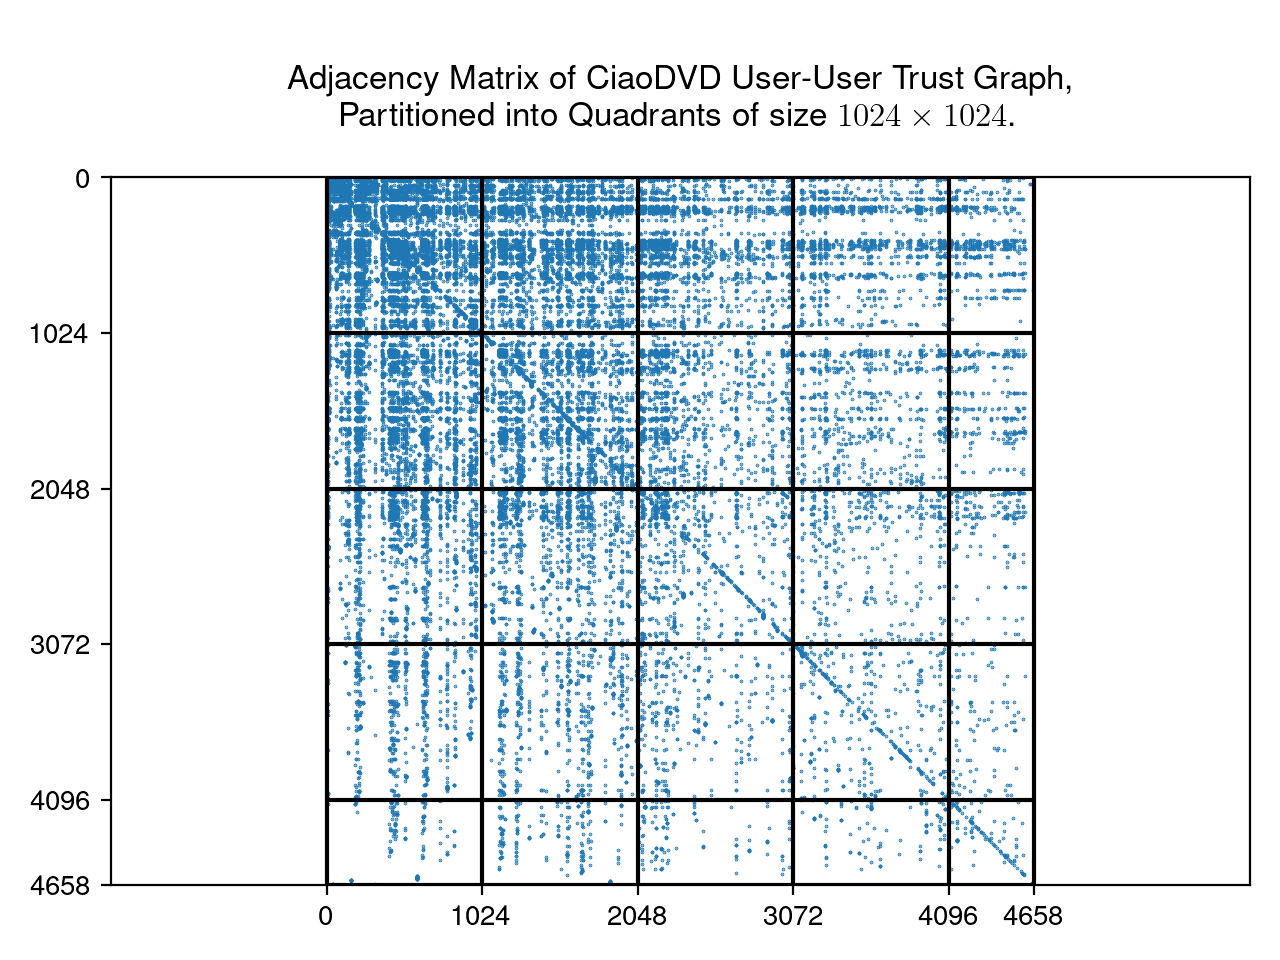
\includegraphics[width=4in]{figures/work_dist_adj_mat.png}
        \label{fig:work_dist_fig}
    }\qquad
    \subfloat[Number of edges per quadrant in Figure \ref{fig:work_dist_fig}.]{
        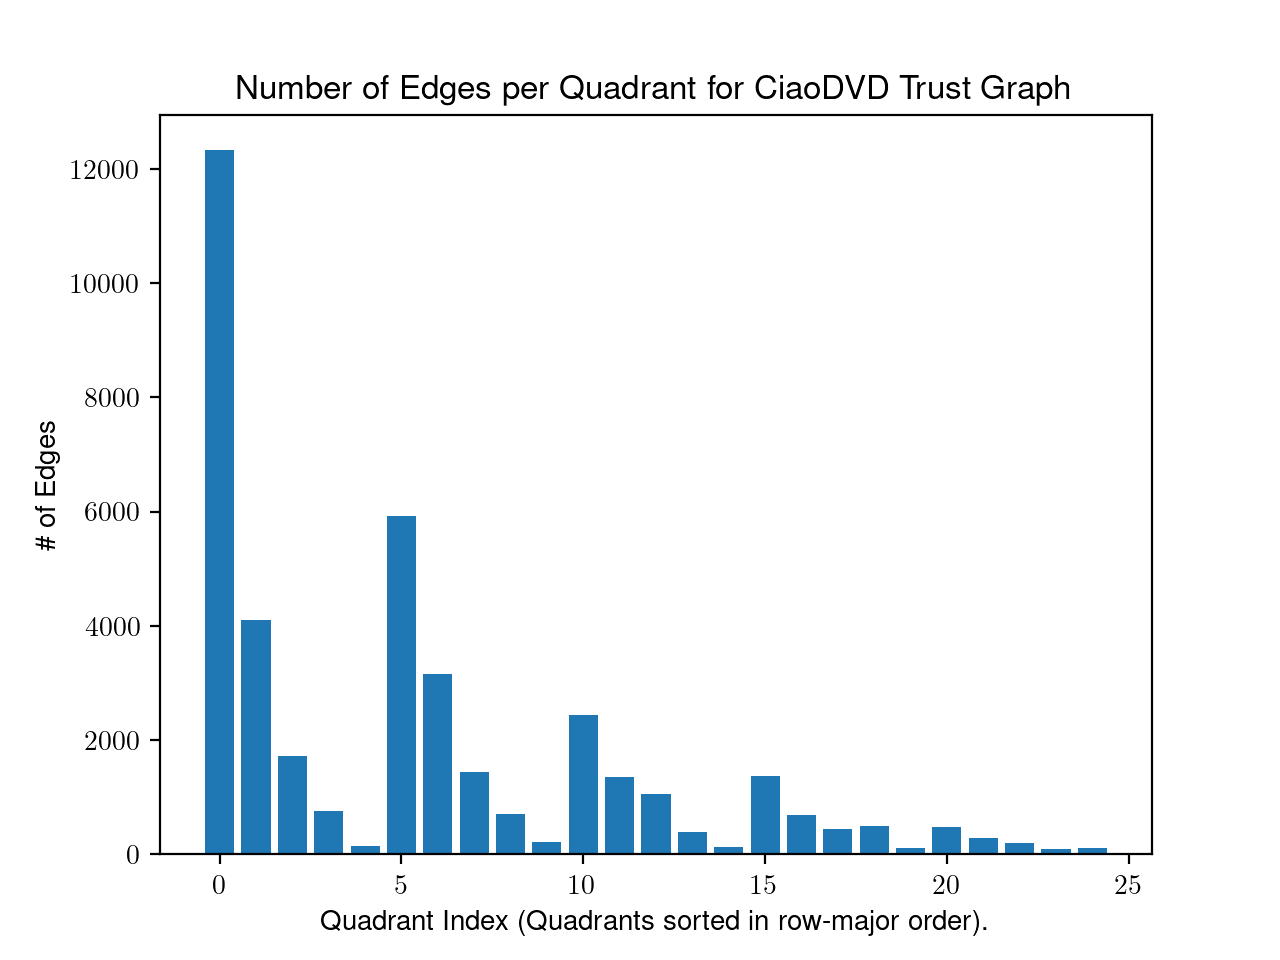
\includegraphics[width=4in]{figures/work_dist.png}
        \label{3figs-c}
    }
    \caption{Uneven distribution of edges due to quadrant partitioning.}
    \label{fig:uneven_work}
\end{figure}
\newpage
\section{Addressing Challenge 1: Efficient Sparse Reductions of Arrays using Spray}
% \AT{
%     I'll start this section by discussing the traditional (and inefficient) way that parallel reductions of
%     arrays was done in OpenMP \cite{openmp}, which is also how previous work (\cite{cagra})
%     attempted to parallelize edge-centric computation using the Hilbert curve. This is where each thread gets its own private copy of the vertex data array, and all thread-private data is merged (e.g. summed) at the end of each iteration. This will motivate my use of Spray \cite{spray} which avoids the allocation of large thread-private arrays by using Block Reductions, and is thus able to scale.
% }
% This chapter addresses Challenge 1: Efficient Sparse Reductions of Arrays using Spray. 
The traditional method of parallel reductions of arrays in OpenMP \cite{openmp} and previous attempts to parallelize edge-centric computation using the Hilbert curve \cite{cagra} have been inefficient: each thread maintained its own private copy of the vertex data array, and all thread-private data was merged (i.e. summed) at the end of each iteration. In this section, we will discuss an alternative approach that uses Block Reductions with Spray \cite{spray}, which avoids the allocation of large thread-private arrays and enables scalability.

\section{Addressing Challenge 2: Recursive Hilbert Blocking}
% \AT{
%     Recursive Hilbert Blocking and Greedy Merging work together to ensure a balanced distribution of edges between blocks. I'll describe the Recursive Hilbert Blocking algorithm and provide pseudo-code for each subsection. Together, all the pseudocode procedures will make up the entire preprocessing algorithm.
%     The final subsection will describe the use of OpenMP dynamic scheduling and chunking. This means that once the final block array has been computed, we dynamically assign groups of consecutive blocks (determined by a hyperparameter, $c$, chunksize), to ensure that the read/write accesses a core makes when iterating over its assigned blocks is limited to a contiguous and cacheable vertex ID range.
% }

This section introduces Recursive Hilbert Blocking, which is an edge reordering and blocking technique 
% used in conjunction with Greedy Merging to 
that ensures a balanced distribution of edges between blocks. In the first two sections we will describe the Recursive Hilbert Blocking algorithm and provide pseudo-code for each of its procedures. Finally, we will discuss the use of OpenMP scheduling and chunking to dynamically assign groups of consecutive blocks (determined by a hyperparameter, $c$, chunksize). This limits the read/write accesses that a core makes when iterating over its assigned blocks to a contiguous and cacheable vertex ID range.

\subsection{Parallel Divide-and-Conquer using OpenMP \texttt{tasks}}
\subsection{Parallel Greedy Merging of Blocks}
\subsection{OpenMP Dynamic Scheduling}

% \section{Edge-Centric Algorithms in Rhubarb}
% In this section we describe how we implemented three Edge-Centric algorithms in Rhubarb. 
% % \AT{dynamic scheduling in OpenMP, and grouping of consecutive blocks in the Hilbert curve.}
% \subsection{PageRank}
% \subsection{Connected Components}
% \subsection{Collaborative Filtering}
% \begin{figure}[!htb]
%     \begin{subfigure}{.5\textwidth}
%       \centering
%       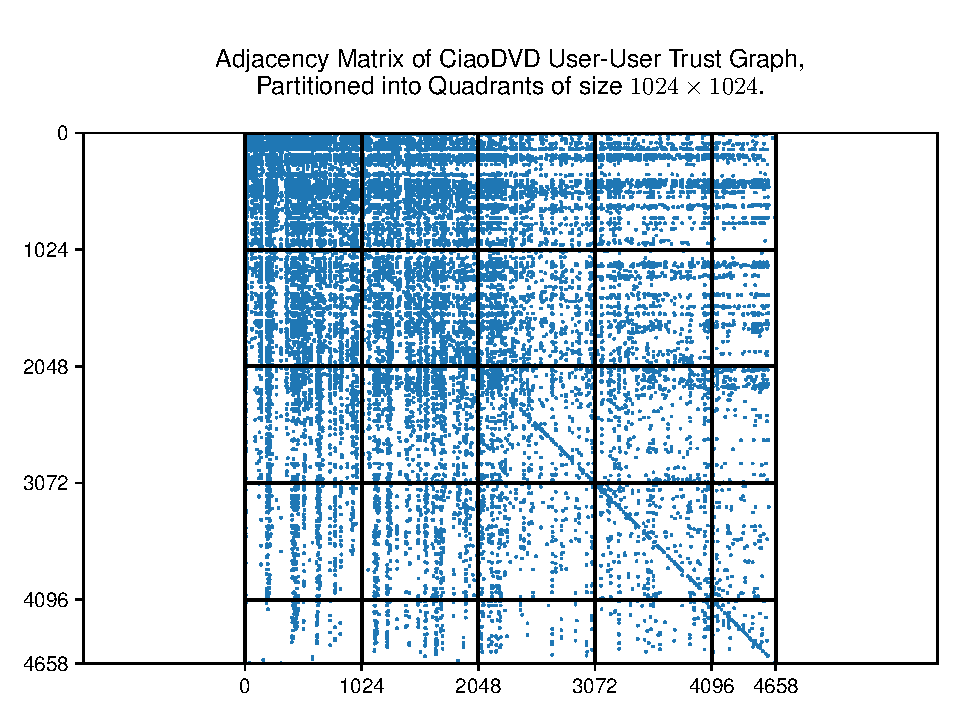
\includegraphics[width=.8\linewidth]{figures/work_dist_adj_mat.pdf}
%       \caption{1a}
%       \label{fig:sfig1}
%     \end{subfigure}%
%     \begin{subfigure}{.5\textwidth}
%       \centering
%       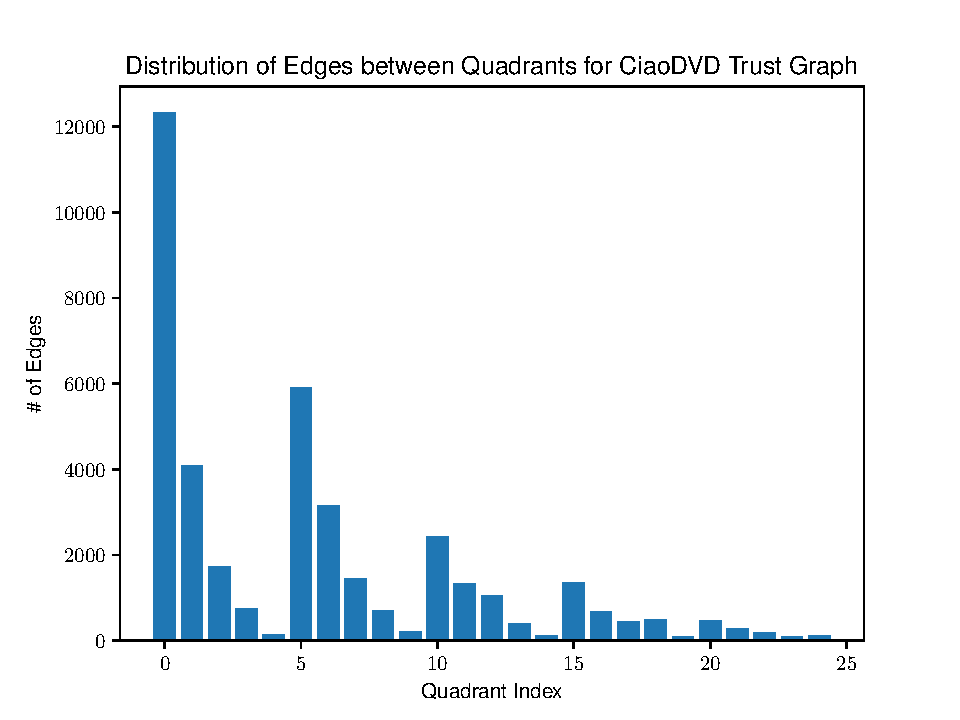
\includegraphics[width=.8\linewidth]{figures/work_dist.pdf}
%       \caption{1b}
%       \label{fig:sfig2}
%     \end{subfigure}
%     \caption{plots of....}
%     \label{fig:uneven_work}
%     \end{figure}

% \algnewcommand{\LineComment}[1]{\State \(\triangleright\) #1}
% \begin{algorithm}
%     \hspace*{\algorithmicindent} \textbf{Input}\\
%     \hspace*{\algorithmicindent}$C$: Graph stored in CSR format \\
%     \hspace*{\algorithmicindent}$C$.index: an $|n|$ array \\
%     \hspace*{\algorithmicindent}$u_0, u_1$: start and end source vertices\\
%     \hspace*{\algorithmicindent}$v_0, v_1$: start and end destination vertices\\
%     \hspace*{\algorithmicindent} \textbf{Output} \\
%     \hspace*{\algorithmicindent} The number of edges in Graph $C$ that lie within the
%     quadrant $[u_0:u_1, v_0:v_1]$
%     \begin{algorithmic}[1]
%         % \LineComment{Given the quadrant specified by the bounds }
%       \Function{n\_edges}{$C, u_0, u_1, v_0, v_1$}  
%     %   \Comment{this is a comment}
%       \State nnz = 0
%       \For{$u$ in range($u0, u1$):}
%       \State neigh\_u\_start = $C$.index[$u$]
%       \State neigh\_u\_end = $C$.index[$u + 1$] \Comment{Start, Endpoint of $u$'s neighbourhood}
%     \LineComment{Binary search to find the index of the first and last out-neighbour }
%     \LineComment{of $u$ that lies in this quadrant}
%       \State first\_idx\_in\_q = lower\_bound($C$.neighbours)
%       \State last\_idx\_in\_q
%         \EndFor 
%       \EndFunction
%     \end{algorithmic}
%   \end{algorithm}
\chapter{Evaluation}
\label{ch:Evaluation}

In the previous chapters we:
\begin{enumerate}
    \item Described the results of our single-threaded PageRank microbenchmark using different Vertex-and-Edge ordering combinations. We saw that specific Vertex-and-Edge orderings (e.g. Slashburn Vertex Order and Hilbert Edge Order) consistently yielded the greatest speedup. This motivated us to parallelize the SlashBurn Vertex Reordering algorithm.
    \item Described the Parallel SlashBurn algorithm and evaluated how well it scales by increasing the number of cores.
          \AT{I think it makes sense to discuss and show the evaluation of how well Parallel Slashburn scales right after I describe how I've implemented it - i.e. at the end of that chapter}.
    \item Described and analyzed RHuBarb (Recursive Hilbert Blocking).
\end{enumerate}

Now, we answer the following Research Questions:

\begin{itemize}
    \item [\textbf{RQ1}] \textit{How expensive is RHuBarb's preprocessing?}
          \begin{itemize}
              \item [\textbf{RQ1.1}] RHuBarb benefits from compressed graph representations (those with a \textit{smaller} number of \textit{denser} blocks, as opposed to a \textit{larger} number of \textit{sparser} blocks.) \textbf{How long do these vertex reorderings take to compute?}
              \item [\textbf{RQ1.2}]{ \textbf{How long does RHuBarb's divide-and-conquer blocking algorithm take?}}
              \item [\textbf{RQ1.3}] \textbf{How well does RHuBarb's divide-and-conquer blocking algorithm scale with an increasing number of cores?}
          \end{itemize}
    \item [\textbf{RQ2}] \textbf{How does RHuBarb compare to State-of-the-Art Graph Processing Systems (GPS)?}
          \AT{This will involve an evaluation of:}
          \begin{enumerate}
              \item Systems: GPOP, Syze, Ligra, GraphMat.
              \item Graphs:
                    \begin{itemize}
                        \item Social Networks: Twitter, Twitter-MPI, Friendster.
                        \item Hyperlink Networks: UK Domain, Wikipedia.
                        \item Road Networks: US Road Network.
                        \item Bipartite User-Item Rating Networks (Specific to Collaborative Filtering benchmark): Yahoo Songs, Amazon.
                    \end{itemize}
              \item Edge-Centric Algorithms:
                    \begin{itemize}
                        \item PageRank, Connected Components, Collaborative Filtering.
                    \end{itemize}
          \end{enumerate}
    \item [\textbf{RQ3}] The performance of RHuBarb depends on 2 user-defined parameters:
    \begin{enumerate}
        \item \textit{$d$, Dynamic Group Size}: How many consecutive Hilbert blocks should be dynamically assigned to cores during Edge-Centric traversal?
        \item \textit{$m$, Maximum Number of Edges per Block}: each Hilbert block must contain \textit{at most} this many edges. 
    \end{enumerate}
    \textbf{How should users choose the values for $d, m$?}
    \item [\textbf{RQ4}] In answering \textbf{RQ2}, we identified a performance bottleneck for SOTA systems (GPOP, SYZE) on graphs whose vertices have been relabelled using the SlashBurn or Descending Degree Sort vertex reorderings (i.e. graphs with ``concentrated edge densities''). Since, given an arbitary input graph, one has no a priori knowledge of the edge density of the graph's ``Original'' vertex ID assignment (except for known examples of Hyperlink networks in the literature), we answer the following:
    \textbf{For graphs whose ``Original'' Vertex ID assignment is ``close'' to a Descending Degree Sort, does RHuBarb perform well out-of-the-box?}\\
    \AT{Or maybe?}
    \textbf{How often are the Vertex IDs of real-world graphs close to a Descending Degree Sort?}
\end{itemize}

We begin this chapter by describing the GPS we'll compare against and the graph datasets and algorithms we'll use in our comparison.
Table \ref{Tab:datasets} lists the graph datasets we used in our evaluation and Sections \ref{sec:ec-algos} and \ref{sec:ggps} briefly describe the algorithms and systems, respectively, and why we chose these specifically.
\crefname{section}{Section}{Sections} % capitalize "E", no period
\crefrangelabelformat{section}{(#3#1#4--#5#2#6)}
\crefrange{sec:preproc}{sec:rank-compare} answer \textbf{RQ1-4}, respectively.

\begin{table}[ht]
    \caption{Graph Datasets}
    \centering
    \hspace*{-2cm}
    \begin{tabular}{ |c| c| c| c | }
        \hline
        Graph            & Description      & $n$        & $m$           \\
        \hline
        \textit{twitter} & Twitter Follower & 41,652,230 & 1,468,365,182 \\
        \hline
        \textit{road} & USA Road & 23,947,347  & 57,708,624  \\
        \hline
        \textit{uk} & Hyperlink Network of .uk Domain & 105,153,952   & 3,301,876,564   \\
        \hline
        \textit{amazon} & Rating Network & 31,050,733    & 82,677,131    \\
        \hline
        \ldots & \ldots & \ldots & \ldots \\
        \hline
    \end{tabular}
    \label{Tab:datasets}
\end{table}





\section{Edge-Centric Graph Algorithms}\label{sec:ec-algos}
\subsection{PageRank}
\subsection{Connected Components}
\subsection{Collaborative Filtering}
\section{Graph Frameworks}\label{sec:ggps}
\subsection{Ligra}
\subsection{GraphMat}
\subsection{GPOP and Syze}

\section{Preprocessing Overhead}\label{sec:preproc}
This section lists the preprocessing time of various vertex reorderings 
\AT{Parallel-SlashBurn, Descending Degree Sort, Degree-Based-Grouping, Rabbit Order, COrder}and Recursive Hilbert-Blocking. We find that certain costly vertex reorderings take longer to compute than certain graph algorithms. In such cases, we also list the number of times the computation must be repeated to amortize the total cost of preprocessing.

\subsection{Cost of Vertex Reorderings}
\subsection{Cost of Recursive Hilbert-Blocking}
\subsection{Scaling of Recursive Hilbert-Blocking}
\subsection{Time to Amortize Costly Preprocessing Steps}
\section{Multicore Comparison} \label{sec:multicore}
This section compares RHuBarb to State-of-the-Art, main-memory GPS.
We compare the performance of RHuBarb to these systems using a representative set of Edge-Centric graph algorithms and graph datasets. Using an increasing number of cores, we measure runtime performance and L2 and LLC cache miss rate.

\AT{A figure like \ref{fig:eval-sample} for PageRank, Connected Components, and Collaborative Filtering. 
(More coloured lines to show the performance of the different systems.)
Also, similar figures to show the L2, LLC Cache-miss rates as we increase the number of cores.
}
\begin{figure}[!htb]
    \centering
    \includegraphics[width=5in]{../plots/eval/twitter-sample.pdf}
    % \includesvg[width=5in]{plots/eval/twitter-sample.svg}
    \caption{Runtime and Scaling for different vertex reorderings (Original, Descending (Out) Degree Sort, and  Slashburn) for PageRank computation using GPOP and Hilbert Blocking.}
    \label{fig:eval-sample}   % label should change
    \end{figure}

\section{Effect of Dynamic Group Size and Minimum Number of Edges per Block}\label{sec:hparams}

In this section, we evaluate the effect of the 2 user-defined parameters of RHuBarb on  performance.

\begin{enumerate}
    \item \textit{$d$, Dynamic Group Size}: How many consecutive Hilbert blocks should be dynamically assigned to cores during Edge-Centric traversal?
    \item \textit{$m$, Maximum Number of Edges per Block}: each Hilbert block must contain \textit{at most} this many edges. 
\end{enumerate}

We perform this performance analysis in order to find a heuristic value for these user-defined parameters.
We evaluate RHuBarb using the combination of $d\in\{1, 2, 4, 8, 16, 32, 64\}$ and 
$m\in\{
    \num[group-separator={,}]{8192}, 
    \num[group-separator={,}]{16384}, 
    \num[group-separator={,}]{32768}, 
    \num[group-separator={,}]{65536}, 
    \num[group-separator={,}]{131072}, 
    \num[group-separator={,}]{262144}
\}$.

Since the combination of $d$ and $m$ dictates the amount of work assigned to each core, we find that the size of the private L2 Cache acts as a good heuristic for a rough upper bound of values to assign to $d$ and $m$. As a result, RHuBarb uses the L2 cache-size at runtime to assign values to $d$ and $m$.

\section{On which graphs does RHuBarb perform well ``out-of-the-box''?}\label{sec:rank-compare}

          \AT{ This is the ``fuzziest'' section in my mind, and is my attempt to answer your note about ``Default orders'' in your email response. I'm not sure how useful the distance metrics I found are for the purpose of comparing the similarity between two vertex reorderings. My current hypothesis is the following:
          }
          \begin{enumerate}
            \item I observed that RHuBarb outperformed SOTA on specific graphs \textbf{without} performing any vertex reordering (i.e. using the original vertex ID assignment). 
            \item I hypothesize that, for these graphs, the ``distance'' between the ``Original'' order and a Descending Degree Sort should be \textbf{smaller} than the distance between Original and Descending Degree Sort for graphs for which we \textit{did} need to sort them to see any performance improvement using RHuBarb.
          \end{enumerate}

          \AT{The distance metrics I'm considering:}
          \begin{itemize}
            \item \textbf{Weighted Kendall Tau Distance}: measures the number of pairwise disagreements between two rankings. It counts the number of times that two items are ranked differently between two rankings. \AT{I can weigh vertex rankings by the vertices' out-degrees. i.e. Vertices with high degrees will contribute more to the final distance scores than vertices with low degree. I don't think this is a good metric, because it simply counts the number of times vertex ID assignment were out of order, not ``how'' out of order they were. For this reason, I think Manhattan distance (below), makes more sense.}
            \item \textbf{Manhattan distance}: calculates the distance between two rankings based on the sum of the absolute differences between the ranks of each vertex.
          \end{itemize}

% \end{document}


%\chapter{Discussion}
\label{ch:discussion}
%\include{conclusions}

%    3. Notes
%    4. Footnotes

%    5. Bibliography
\begin{singlespace}
  \raggedright
  \bibliographystyle{abbrvnat}
  \bibliography{biblio}
\end{singlespace}

\appendix
%    6. Appendices (including copies of all required UBC Research
%       Ethics Board's Certificates of Approval)
%\include{reb-coa}	% pdfpages is useful here
\include{appendix}

\backmatter
%    7. Index
% See the makeindex package: the following page provides a quick overview
% <http://www.image.ufl.edu/help/latex/latex_indexes.shtml>


\end{document}
